%\documentclass[11pt,a4paper,twoside]{tesis}
% SI NO PENSAS IMPRIMIRLO EN FORMATO LIBRO PODES USAR
\documentclass[12pt,a4paper]{tesis}

% Paquetes para figuras y subfiguras
\usepackage{graphicx}
\usepackage{caption}
\usepackage{subcaption}

% Codificacion de los caracteres
\usepackage[utf8]{inputenc}

% Configuracion de babel
\def\spanishoptions{activeacute}
\usepackage[english, spanish]{babel}




% Espaciado
%\usepackage[left=3cm,right=3cm,bottom=3.5cm,top=3.5cm]{geometry}
\linespread{1.3}

%%%%%%%%%%%%%%%%%%%%%%%
% Para los comentarios
%%%%%%%%%%%%%%%%%%%%%%%
\usepackage{xspace}
\usepackage[colorinlistoftodos, shadow]{todonotes}
%\usepackage[disable]{todonotes}
\newcommand{\comentarioM}[1]{\todo[bordercolor=green!20, color=green!20, inline]{mbianchi: #1}\xspace}
\newcommand{\comentarioiM}[1]{\todo[bordercolor=green!20, color=green!20, linecolor=black!40]{mbianchi: #1}\xspace}
\newcommand{\comentarioP}[1]{\todo[bordercolor=yellow!20, color=yellow!20, inline]{pachi: #1}\xspace}

\newcommand{\comentarioxP}[1]{\comentarioP{\sout{#1}}}
\newcommand{\comentarioxM}[1]{\comentarioM{\sout{#1}}}

%%%%%%%%%%%%%%%%%%%%%%%
% Otros
%%%%%%%%%%%%%%%%%%%%%%%
\newcommand{\param}[1]{\textbf{\uppercase{#1}}}
\newcommand{\ap}{\textit{alignment prerejective}}
\newcommand{\kdt}{\textit{k-dtree}}

\begin{document}

%%%% CARATULA
\def\titulo{Licenciado }
\def\autor{Mariano Bianchi}
\def\tituloTesis{Seguimiento de Objetos en Secuencias de Imágenes RGB-D}
\def\runtitulo{Seguimiento de Objetos en Secuencias de Imágenes RGB-D}
\def\runtitle{Object tracking using RGB-D image sequences}
\def\director{Francisco Roberto Gómez Fernández}
%\def\codirector{Master Yoda}
\def\lugar{Buenos Aires, 2014}
\newcommand{\HRule}{\rule{\linewidth}{0.2mm}}
%
\thispagestyle{empty}

\begin{center}\leavevmode

\vspace{-2cm}

\begin{tabular}{l}

\includegraphics[width=2.6cm]{logofcen.pdf}
\end{tabular}


{\large \sc Universidad de Buenos Aires

Facultad de Ciencias Exactas y Naturales

Departamento de Computaci\'on}

\vspace{6.0cm}

%\vspace{3.0cm}
%{
%\Large \color{red}
%\begin{tabular}{|p{2cm}cp{2cm}|}
%\hline
%& Pre-Final Version: \today &\\
%\hline
%\end{tabular}
%}
%\vspace{2.5cm}

{\huge\bf \tituloTesis}

\vspace{2cm}

{\large Tesis presentada para optar al t\'{\i}tulo de\\
\titulo en Ciencias de la Computaci\'on}

\vspace{2cm}

{\Large \autor}

\end{center}

\vfill

{\large

{Director: \director}

\vspace{.2cm}

{Codirector: \codirector}

\vspace{.2cm}

\lugar
}

\newpage\thispagestyle{empty}


%%%% ABSTRACTS, AGRADECIMIENTOS Y DEDICATORIA
\frontmatter
\pagestyle{empty}
\chapter*{\runtitulo}

% Acá iría el abstract en español (aprox. 200 palabras).
\noindent Actualmente las aplicaciones de métodos de seguimiento son muchas y su utilización aplica en diversos contextos, desde procesos industriales a entretenimiento. La creciente popularización de sensores RGB-D provoca un gran interés científico para aplicar nuevas técnicas de procesamiento de imágenes y adaptar otras conocidas a la enriquecida información que proveen estos sensores. Estos proveen información de profundidad en conjunto con texturas RGB de forma sincronizada y a una frecuencia de 30 cuadros por segundo, permitiendo obtener aplicaciones en tiempo real. En este trabajo presentamos un sistema de seguimiento separado en tres etapas y distintos métodos de detección y seguimiento en RGB, en profundidad y en su combinación. Utilizando datos de \textit{ground truth} obtenidos de una base de datos de escenas y objetos analizamos el funcionamiento de nuestro sistema



\bigskip

\noindent\textbf{Palabras claves:} tracking RGB-D, sistema de seguimiento, ICP, \textit{template matching}, estimación de pose, alineación, (no menos de 5)


\cleardoublepage
%\begin{center}
%\large \bf \runtitle
%\end{center}
%\vspace{1cm}
\chapter*{\runtitle}

\noindent In a galaxy far, far away, a psychopathic emperor and his most trusted servant -- a former Jedi Knight known as Darth Vader -- are ruling a universe with fear. They have built a horrifying weapon known as the Death Star, a giant battle station capable of annihilating a world in less than a second. When the Death Star's master plans are captured by the fledgling Rebel Alliance, Vader starts a pursuit of the ship carrying them. A young dissident Senator, Leia Organa, is aboard the ship \& puts the plans into a maintenance robot named R2-D2. Although she is captured, the Death Star plans cannot be found, as R2 \& his companion, a tall robot named C-3PO, have escaped to the desert world of Tatooine below. Through a series of mishaps, the robots end up in the hands of a farm boy named Luke Skywalker, who lives with his Uncle Owen \& Aunt Beru. Owen \& Beru are viciously murdered by the Empire's stormtroopers who are trying to recover the plans, and Luke \& the robots meet with former Jedi Knight Obi-Wan Kenobi to try to return the plans to Leia Organa's home, Alderaan. After contracting a pilot named Han Solo \& his Wookiee companion Chewbacca, they escape an Imperial blockade. But when they reach Alderaan's coordinates, they find it destroyed - by the Death Star. They soon find themselves caught in a tractor beam \& pulled into the Death Star. Although they rescue Leia Organa from the Death Star after a series of narrow escapes, Kenobi becomes one with the Force after being killed by his former pupil - Darth Vader. They reach the Alliance's base on Yavin's fourth moon, but the Imperials are in hot pursuit with the Death Star, and plan to annihilate the Rebel base. The Rebels must quickly find a way to eliminate the Death Star before it destroys them as it did Alderaan (aprox. 200 palabras).

\bigskip

\noindent\textbf{Keywords:} War, Rebellion, Wookie, Jedi, The Force, Empire (no menos de 5).

\cleardoublepage
\chapter*{Agradecimientos}
\begin{itemize}
    \item A mi director Francisco Roberto Gómez Fernández, Pachi para todo el mundo, por su paciencia infinita desde el día cero. Desde que nos sentamos a tomar un café para charlar sobre qué temas de imágenes podían llegar a interesarme hasta el día antes de la defensa de tesis se mostró alegre, entusiasmado y sobre todo, con muchas ganas de guiarme y ayudarme. ¡Gracias Pachi!
    \item A mis viejos, Victor y Sonia, por bancarme todos estos años tanto emocionalmente como monetariamente. Sin su apoyo esto no hubiera sido posible.
    \item A mi hermanita mayor, Paola, por acompañarme siempre y por tantos años lindos de convivencia juntos en Capital.
    \item Al bombonazo de mi novia, Natalin, por todo el aguante incondicional. Por bancarme todos estos años de carrera, algunos de los cuales me aguantó un poco loco. Gracias por recorrer este largo camino a mi lado, por tantas charlas interminables dándome aliento para no aflojar.
    \item A mi tío Willy, por haber cedido desinteresadamente su departamento para usarlo de bunker de estudio todos estos años. Claramente no hubiese sido tan fácil el camino sin haber recibido semejante ayuda. ¡Gracias infinitas!
    \item A mis amigos de la vida: Juani, ``el negro'', ``el rubio'', Fede, Luis, Nico, Gustav. Gracias por tantas juntadas, mateadas, asados, pileteadas, voleys y un largo etcétera que hicieron que los momentos libres de todos estos años no tuvieran desperdicio.
    \item A Pablo Brusco, compañero y amigo desde el inicio de la carrera. Por tantas juntadas dentro y fuera de la facultad, por estudio o por ocio. Siempre con su característica buena onda para que este largo viaje fuese un viaje de placer en primera clase. Sin él la facultad no hubiese sido tan entretenida y claramente hubiese sido un viaje mucho más largo.
    \item A Matías López y Rosenfeld, por tantas mateadas, consejos, charlas, fernets y bicicleteadas hasta la facultad juntos. Pasó de ser uno de mis primeros docentes en la carrera a un gran amigo.
    \item A todos los compañeros de cursada que me acompañaron durante toda o gran parte de la carrera y amigos que fui encontrando en la facultad en todos estos años (algunos de los cuales ya les perdí el rastro). Seguro me voy a saltear alguno pero intentaré hacer una lista extensiva: Carlos, Kevin, Thomas, Fede Pousa, Facu Carrillo, Pablo Echevarría, Dani Nuss, Julian, Agus Montero, ``Pape'', Martín, Mariano S., Herman, Caro Hadad, Carla, Fran Giménez, Mica, Nico ``el salteño'', Pablo Laciana, Viviana, Nacho Vissani, Nico Rosner
    \item A mis amigos matemáticos: Eli, Flor, Anto, Juanma. Por todos estos años de amistad y tantas alegrías compartidas.
    \item A todo el DC, desde los profesores, jtps y ayudantes hasta los admines y administrativos, por hacer del DC una casa de estudios de primerísimo nivel académico y por sobre todas las cosas, una gran familia.
\end{itemize}
 % OPCIONAL: comentar si no se quiere

%\cleardoublepage
%\hfill \textit{A mi viejo.}  % OPCIONAL: comentar si no se quiere

\cleardoublepage
\tableofcontents

\mainmatter
\pagestyle{headings}




En la actualidad, las posibles aplicaciones de métodos de seguimiento o tracking son muchas y van desde el uso en la industria hasta juegos de consola. Un ejemplo de ello es la fabricación de barcos y autos mediante el uso de robots. Estas tareas se caracterizan por la necesidad de posicionar de manera precisa una herramienta sobre una pieza de trabajo. A través del uso de métodos de tracking se puede conocer la posición y pose de la pieza que se desea utilizar con respecto a la pose de la cámara y de esta forma saber cómo ubicar la herramienta necesaria para trabajar sobre la pieza en cuestión.

Otra área en donde se utiliza tracking de objetos es para la generación de estadísticas durante un partido de fútbol, tanto de jugadores como de un equipo, aunque las posibles aplicaciones en este contexto son mucho más amplias, como por ejemplo análisis de tácticas, verificación de las decisiones del árbitro, resúmenes automáticos de un partido, etc.

Actualmente existen sensores de profundidad que en conjunto con una cámara RGB pueden ser utilizados para detectar y seguir a una o más personas en tiempo real. De esta manera, mediante un sistema que procese las imágenes RGB-D de estos sensores, las personas puedan utilizar su cuerpo y sus movimientos para interactuar naturalmente con un dispositivo.

La utilización de sensores RGB-D se ha popularizado en los últimos años, cobrando un gran interés científico el estudio de aplicaciones y métodos capaces de procesar y entender la información que los mismos proveen.

La información de profundidad que nos provee un sensor RGB-D es un dato fundamental que nos posibilita encontrar la distancia de un objeto al sensor pudiendo recuperar su información 3D (tridimensional) junto a su textura RGB en tiempo real: 30 cuadros por segundo.
El video RGB-D que se obtiene provee una gran ayuda al mejoramiento y desarrollo de nuevas técnicas de procesamiento de imágenes y video ya conocidas. En particular, es de interés en esta tesis, el seguimiento de objetos en secuencias de imágenes RGB-D.

Un sistema de seguimiento se puede dividir en tres etapas bien definidas:
\begin{enumerate}
 \item Entrenamiento
 \item Detección
 \item Seguimiento cuadro a cuadro
\end{enumerate}

La etapa de entrenamiento consiste en obtener una representación del objeto al cuál se pretende seguir. Para llevarla a cabo se puede utilizar un patrón (template) ya conocido o aprenderlo de imágenes capturadas del mismo objeto. Este template luego se utiliza en la detección para ubicar la representación del objeto dentro de una imagen cualquiera. Una vez conocido el template no se requiere de una nueva ejecución del entrenamiento.

La segunda etapa, la de detección, radica en encontrar dentro de un frame del video al objeto en cuestión utilizando el método de detección deseado, valiéndose de la información registrada en la etapa de entrenamiento. Esta etapa se ejecuta, con el propósito de encontrar en la imagen el objeto a seguir, al comienzo del sistema de seguimiento y cuando el seguimiento cuadro a cuadro falla. Dado que la etapa de detección suele ser la más costosa en términos de desempeño computacional es deseable que se ejecute la menor cantidad de veces posible.

Finalmente, la tercera etapa consiste en seguir cuadro a cuadro el objeto detectado en la etapa anterior. Es decir, teniendo la ubicación del objeto en un cuadro de video se desea identificar la posición del mismo objeto en el siguiente frame. Esta etapa es la más importante ya que es la que se ejecuta en cada frame del video. La eficiencia del método de seguimiento es lo que determinará que todo el sistema de seguimiento se consiga realizar eficientemente. Si la técnica de seguimiento tiene una efectividad baja, es decir, no logra identificar la nueva posición del objeto en el siguiente cuadro, se debe volver a la etapa de detección cuyo desempeño computacional es mayor.


\section{Objetivos ¿va?}

El objetivo principal de esta tesis es la implementación, estudio y evaluación de un sistema de seguimiento de objetos en secuencias de imágenes RGB-D, con las siguientes características:
\begin{itemize}
 \item Performance Real-time: procesamiento de imágenes mayor a 10 cuadros por segundo
 \item Seguimiento de objetos tridimensionales con forma conocida previamente y de objetos aprendidos mediante una fase de entrenamiento previa
 \item Funcionamiento en sensores de profundidad de bajo costo (Kinect, XTion, etc.)
\end{itemize}


\chapter{Sistema de seguimiento en video}

Un sistema de seguimiento en video se puede dividir en tres etapas bien definidas:
\begin{enumerate}
 \item Entrenamiento
 \item Detección
 \item Seguimiento cuadro a cuadro
\end{enumerate}

La etapa de entrenamiento consiste en obtener una representación del objeto al cuál se pretende seguir. Para llevarla a cabo se puede utilizar un patrón \textit{template} ya conocido o aprenderlo de imágenes capturadas del mismo objeto. Luego, este se utilizará en la detección para ubicar la representación del objeto dentro de una imagen cualquiera. Una vez conocido el \textit{template} no se requiere de una nueva ejecución del entrenamiento.

La segunda etapa, la de detección, radica en encontrar dentro de un cuadro del video al objeto en cuestión utilizando el método de detección deseado, valiéndose de la información obtenida en la etapa de entrenamiento. Esta etapa se ejecuta, con el propósito de encontrar en la imagen el objeto a seguir, al comienzo del sistema de seguimiento y cuando el seguimiento cuadro a cuadro falla. Dado que la etapa de detección suele ser la más costosa en términos de desempeño computacional es deseable que se ejecute la menor cantidad de veces posible.

Finalmente, la tercera etapa consiste en seguir cuadro a cuadro el objeto detectado en la etapa anterior. Es decir, teniendo la ubicación del objeto en un cuadro de video se desea identificar la posición del mismo objeto en el siguiente \textit{frame}. Esta etapa es la más importante ya que es la que se ejecuta en cada frame del video. La eficiencia del método de seguimiento cuadro a cuadro es lo que determinará que todo el sistema de seguimiento se consiga realizar eficientemente. Si la técnica de seguimiento tiene una efectividad baja, es decir, no logra identificar la nueva posición del objeto en el siguiente cuadro, se debe volver a la etapa de detección degradando el desempeño de todo el sistema.

Tomando como base estas etapas, proponemos distintos métodos para cada una de ellas tanto para imágenes sólo RGB, como para \textit{depth} (profundidad) y la combinación RGB-D. La primera etapa del sistema puede ser prescindible si contamos con el modelo RGB-D del objeto a seguir y una cámara calibrada. Este es el caso de estudio de esta tesis, ya que, con el propósito de poder evaluar cuantitativamente el seguimiento de objetos en secuencias de imágenes RGB-D, utilizamos la base de datos con ground truth descripta en la sección \ref{base_rgbd}.

\section{Método propuesto RGB}\label{metodo_rgb}
En esta sección explicaremos como se implementó el sistema de seguimiento para secuencias de imágenes RGB basándonos en las etapas explicadas previamente.

\subsection{Entrenamiento}
La etapa de entrenamiento en este método consta de tomar de la base de datos cuatro templates del objeto que se desea seguir con sus respectivas máscaras. Cada uno de los templates corresponde a una pose distinta. Primero se elige de manera arbitraria una de las varias escenas por objeto que tiene la base de datos. Una vez elegida la escena se toman cuatro templates de manera que se cubran las distintas caras del objeto. Si se toma la primer imagen de la escena como la imagen con rotación 0 el resto de las imagenes se eligieron de manera tal que cada una difiera de la anterior en 90 grados. En la figura \ref{templates_objeto} se pueden ver los distintos templates tomados de esta manera para un objeto de la base de datos. Una vez almacenados estos templates y sus respectivas máscaras se pasa a la etapa de detección.

\begin{figure}
	\centering
	\begin{subfigure}[b]{0.25\textwidth}
		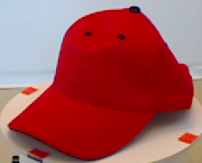
\includegraphics[width=\textwidth]{img/0_crop.png}
		\caption{Rotacion $0^{\circ}$}
	\end{subfigure}
	\quad
	\begin{subfigure}[b]{0.25\textwidth}
		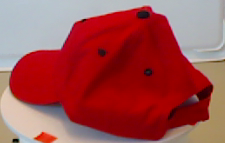
\includegraphics[width=\textwidth]{img/90_crop.png}
		\caption{Rotacion $90^{\circ}$}
	\end{subfigure}

	\begin{subfigure}[b]{0.25\textwidth}
		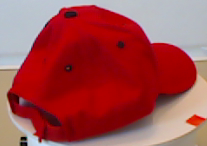
\includegraphics[width=\textwidth]{img/180_crop.png}
		\caption{Rotacion $180^{\circ}$}
	\end{subfigure}
	\quad
	\begin{subfigure}[b]{0.25\textwidth}
		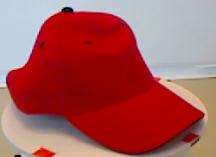
\includegraphics[width=\textwidth]{img/270_crop.png}
		\caption{Rotacion $270^{\circ}$}
	\end{subfigure}
	\caption{Templates de una gorra tomados de la base de datos}
	\label{templates_objeto}
\end{figure}

\subsection{Detección}
Dada la información provista por la base de datos, aprovechada durante el entrenamiento, resulta natural utilizar como método de detección el algoritmo de \textit{Template matching}. \comentarioM{Hay que explicarlo, ¿no?} La implementación utilizada es la que se encuentra presente en la librería \textit{OpenCV} para C++. Esta implementación recibe varios parámetros. El primero es el frame de la escena a donde se desea detectar el objeto. El segundo es el template con el que se va a buscar el objeto. El tercero es opcional y es una máscara para el template del objeto. En este caso como tenemos la máscara disponible este parámetro lo usamos. El último parámetro le indica al algoritmo de template matching que comparación usar para matchear el template a la imagen. Nosotros decidimos utilizar la diferencia cuadrática pixel por pixel normalizada, descripta por la siguiente fórmula:

\comentarioM{Insertar formula aqui.}% http://docs.opencv.org/modules/imgproc/doc/object_detection.html?highlight=matchtemplate#matchtemplate

Pero aplicar este método de manera directa no es suficiente. El problema principal es que la escena de donde se obtuvieron los templates y máscaras del objeto a buscar no es la misma escena que la que se utiliza para verificar el comportamiento del sistema. Esto significa que las poses del objeto tomadas en la etapa de entrenamiento pueden ser completamente distintas a las poses del objeto en la escena en donde se aplica el sistema de seguimiento. Además, la distancia de la cámara al objeto en la escena de búsqueda varía constantemente y difiere de la distancia entre ambos en la escena de donde se capturó el modelo del objeto. Por este motivo también va diferir la escala del objeto en cada escena.

Teniendo en cuenta estos problemas decidimos realizar varias corridas del algoritmo de \textit{template matching}. En primera medida en cada pasada se va modificando el par template-máscara utilizados como parámetros del mismo aprovechando los datos obtenidos en la etapa de entrenamiento. Con esto se ataca de mejor manera el problema de las distintas poses en las que puede estar el objeto en la escena. Además, para que la detección sea más robusta frente a cambios de tamaño del objeto que se desea encontrar se toma a cada uno de los templates con su respectiva máscara y se les aplican varios cambios de escala y se utilizaron estas muestras como entrada para el algoritmo de template matching. Una vez corrido el algoritmo para cada par template-máscara, se obtiene como resultado final la corrida que tenga menor diferencia cuadrática y que esté por debajo de un umbral predefinido. La información que se almacena como resultado son las coordenadas del cuadrante que contiene al objeto encontrado. Una vez almacenada esta información, el sistema pasa a la etapa de seguimiento.

\subsection{Seguimiento}\label{tracking_rgb}
Como se explicó al comienzo del capítulo, esta etapa consta de seguir al objeto detectado en la etapa anterior frame a frame. Para concretar este objetivo se necesita encontrar una manera de combinar la información obtenida durante las dos etapas anteriores. Existen muchas maneras de llevar a cabo esta tarea. La forma que elegimos para este trabajo fue utilizar un método de comparación por histogramas.

Cada imagen RGB consta de tres imagenes, una por cada canal. Para calcular el histograma de una imagen se toman los distintos valores (intensidad) de cada pixel y se cuenta la cantidad de veces que se repite cada uno de esos valores en la imagen. Las imágenes que utilizamos durante el transcurso de este trabajo son de 8 bits por pixel, por lo que cada pixel puede tomar un valor entre 0 y 255. Para que las comparaciones entre histogramas sean más robustas lo que se decidió fue trabajar con histogramas normalizados.


\begin{figure}
	\centering
	\begin{subfigure}[b]{0.25\textwidth}
		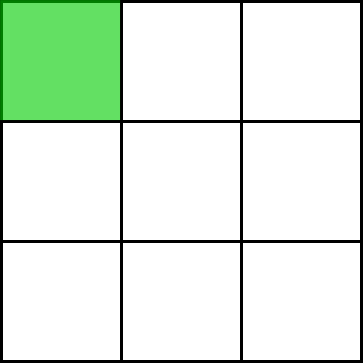
\includegraphics[width=\textwidth]{img/primercuadrante.png}
		\caption{Primer frame de búsqueda}
		\label{frames_solapados_1}
	\end{subfigure}
	\quad
	\begin{subfigure}[b]{0.25\textwidth}
		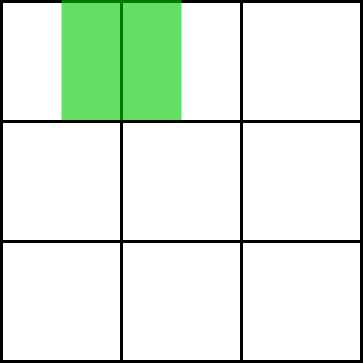
\includegraphics[width=\textwidth]{img/segundocuadrante.png}
		\caption{Segundo frame de búsqueda}
		\label{frames_solapados_2}
	\end{subfigure}
	\quad
	\begin{subfigure}[b]{0.25\textwidth}
		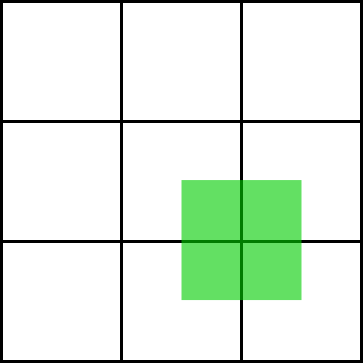
\includegraphics[width=\textwidth]{img/decimonovenocuadrante.png}
		\caption{$19^{\circ}$ frame de búsqueda}
		\label{frames_solapados_3}
	\end{subfigure}
	\caption{Se busca en cada cuadrante de la grilla y en los recuadros del mismo tamaño que cubren los bordes de la grilla principal}
	\label{frames_solapados}
\end{figure}


El algoritmo de tracking implementado se puede separar en dos partes. Por un lado tenemos el método de búsqueda y por el otro el algoritmo de comparación por histogramas. El método de búsqueda se utiliza para explorar un espacio predefinido en donde se asume estará el objeto en el siguiente frame. Este algoritmo toma un área de tamaño 9 veces mayor a la del cuadrante reportado por el algoritmo de detección respetando el centro del mismo. Luego divide esta área en cuadrantes los que serán utilizados por el algoritmo de comparación para definir si el objeto está o no allí. En la figura \ref{frames_solapados} se muestra una secuencia de búsqueda por cuadrantes. Para hacer más robusta la búsqueda frente a cambios de tamaño del objeto este mismo método de búsqueda por cuadrantes se realiza varias veces cambiando el tamaño del cuadrante.

La segunda parte del algoritmo de tracking consta en definir cuál de todos los cuadrantes explorados en la etapa de búsqueda es el que contiene el objeto que se está buscando o en caso de fallar en la búsqueda, indicar que el objeto no se encontró en el frame. En un principio en esta etapa se comparaba el histograma de cada uno de los cuadrantes explorados con el cuadrante del frame anterior reportado por el algoritmo de detección. Para esta comparación se tomaba de cada recuadro su histograma para los canales S y V del esquema de colores HSV y se los comparaba utilizando la implementación de comparación de histogramas presente en la librería OpenCV. El método de comparación utilizado se basaba en la diferencia de \textit{Bhattachayyra}. El resultado de estas comparaciones era aquel cuadrante cuya comparación arrojara el menor valor y que se encontrara por debajo de un umbral definido. Si ningún cuadrante arrojaba una comparación menor a este umbral el algoritmo indicaba que el objeto no se encontraba en ese frame.

El problema con esta aproximación era que al basarse únicamente en el recuadro encontrado en el frame anterior el objeto iba quedando de a poco fuera del recuadro resultante hasta que en un momento quedaba completamente fuera del mismo. Como la diferencia entre los cuadrantes resultantes de cada frame era baja, el algoritmo seguía reportando al objeto como encontrado aunque no fuera así. Para evitar este inconveniente se decidió además comparar el histograma de cada cuadrante de búsqueda con el histograma de uno de los templates del objeto obtenido en la etapa de entrenamiento. En este caso la comparación se realizó utilizando el esquema RGB, calculando el histograma para los tres canales. En las figuras \ref{frame_only_tracking} y \ref{frame_template_tracking} se pueden ver dos secuencias del algoritmo de seguimiento, una con comparación de histogramas unicamente entre frame y frame y otra que agrega además la comparación con el template del objeto respectivamente. El cuadrante de color verde es el reportado por el ground truth como la ubicación del objeto en la escena, en este caso, una taza. El cuadrante de color azul es el reportado por nuestro algoritmo. En la figura \ref{frame_only_tracking} podemos ver como frame a frame el cuadrante azul se va alejando de la taza hasta que en el frame 8 de este extracto de la escena el algoritmo indica que encontró a la taza en una zona que en realidad es parte de la notebook. En la figura \ref{frame_template_tracking} podemos ver en cambio que el área reportada por el algoritmo se mantiene más estable. En el frame 7 aparece un recuadro rojo. Eso significa que el algoritmo de seguimiento perdió el rastro del objeto y en ese frame hizo falta correr el algoritmo de detección. Luego, en los frames 8 y 9 el algoritmo no reporta haber seguido al objeto. Por este motivo es que se decidió utilizar la comparación de histogramas tanto con el frame anterior como con el template del objeto.

\comentarioM{¿Explico porque se eligió HSV y RGB en cada caso?}

\begin{figure}
	\centering
	\begin{subfigure}[b]{0.3\textwidth}
		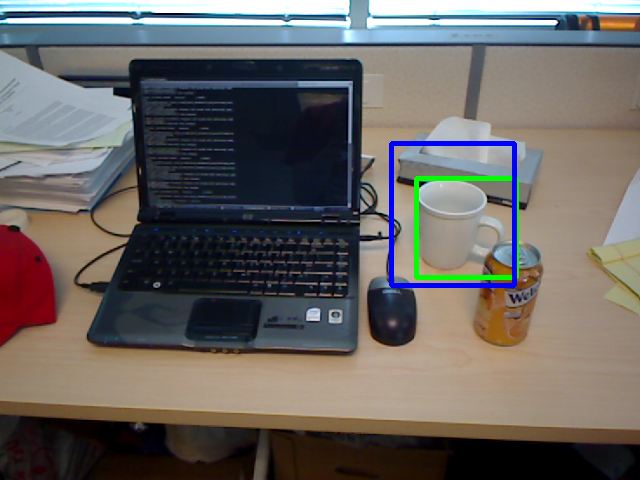
\includegraphics[width=\textwidth]{img/seguimiento_solo_frame/solo_frame-desk_1-coffee_mug_5-frame_26.png}
	\end{subfigure}
	\begin{subfigure}[b]{0.3\textwidth}
		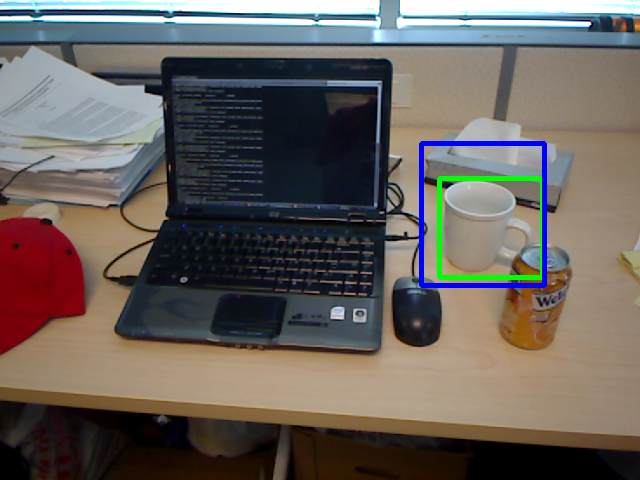
\includegraphics[width=\textwidth]{img/seguimiento_solo_frame/solo_frame-desk_1-coffee_mug_5-frame_27.png}
	\end{subfigure}
	\begin{subfigure}[b]{0.3\textwidth}
		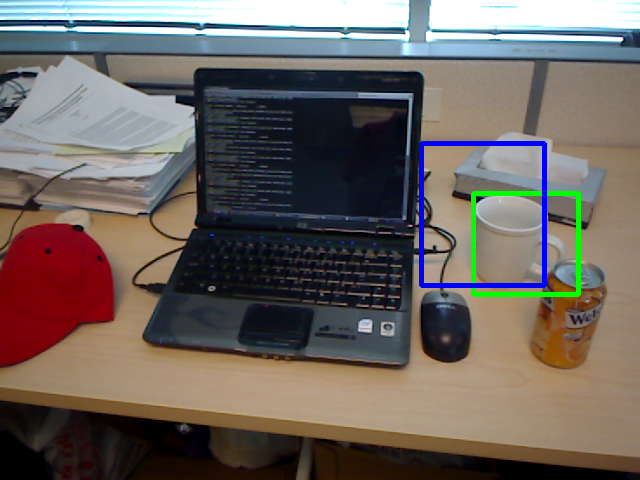
\includegraphics[width=\textwidth]{img/seguimiento_solo_frame/solo_frame-desk_1-coffee_mug_5-frame_28.png}
	\end{subfigure}


	\begin{subfigure}[b]{0.3\textwidth}
		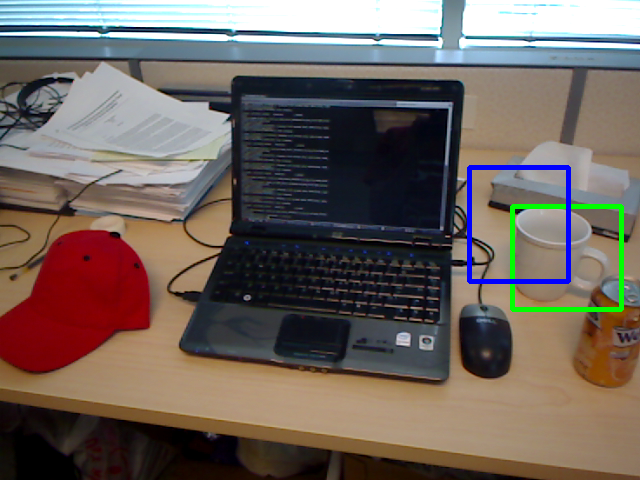
\includegraphics[width=\textwidth]{img/seguimiento_solo_frame/solo_frame-desk_1-coffee_mug_5-frame_29.png}
	\end{subfigure}
	\begin{subfigure}[b]{0.3\textwidth}
		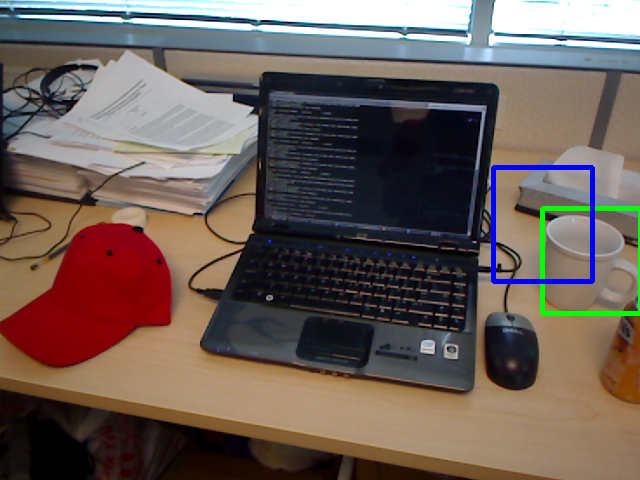
\includegraphics[width=\textwidth]{img/seguimiento_solo_frame/solo_frame-desk_1-coffee_mug_5-frame_30.png}
	\end{subfigure}
	\begin{subfigure}[b]{0.3\textwidth}
		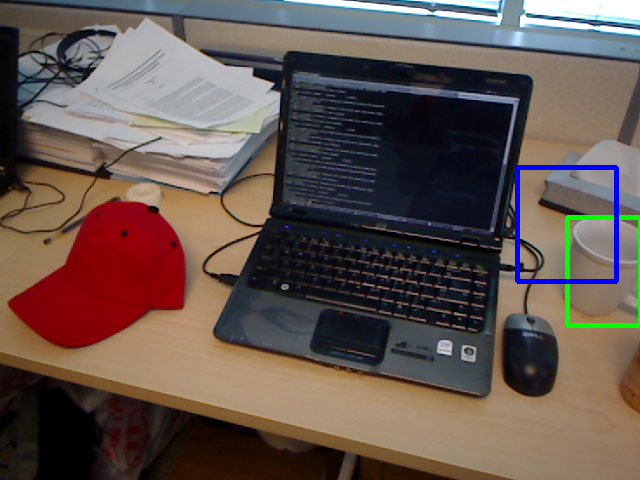
\includegraphics[width=\textwidth]{img/seguimiento_solo_frame/solo_frame-desk_1-coffee_mug_5-frame_31.png}
	\end{subfigure}

	\begin{subfigure}[b]{0.3\textwidth}
		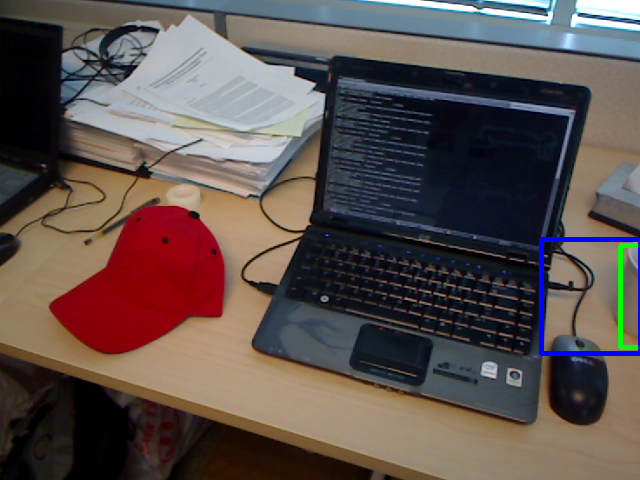
\includegraphics[width=\textwidth]{img/seguimiento_solo_frame/solo_frame-desk_1-coffee_mug_5-frame_32.png}
	\end{subfigure}
	\begin{subfigure}[b]{0.3\textwidth}
		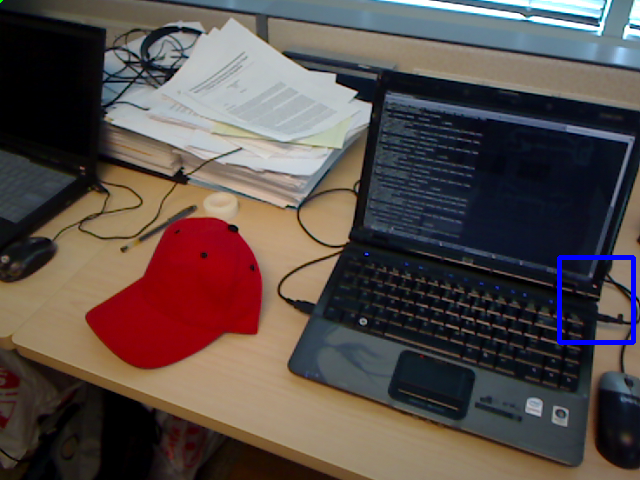
\includegraphics[width=\textwidth]{img/seguimiento_solo_frame/solo_frame-desk_1-coffee_mug_5-frame_33.png}
	\end{subfigure}
	\begin{subfigure}[b]{0.3\textwidth}
		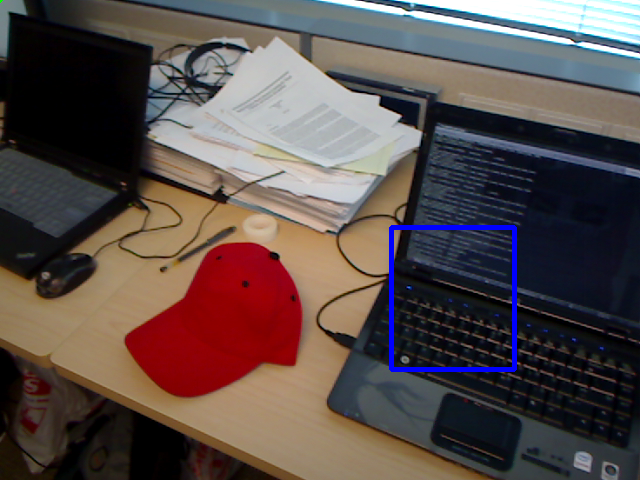
\includegraphics[width=\textwidth]{img/seguimiento_solo_frame/solo_frame-desk_1-coffee_mug_5-frame_34.png}
	\end{subfigure}

	\caption{Seguimiento frame a frame divergiendo. Aquí se estaba usando solo comparación de histogramas entre el frame anterior y el actual}
	\label{frame_only_tracking}
\end{figure}


\begin{figure}
	\centering
	\begin{subfigure}[b]{0.3\textwidth}
		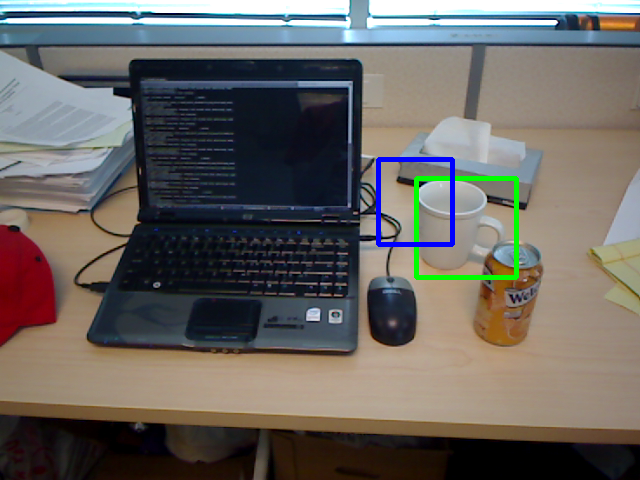
\includegraphics[width=\textwidth]{img/seguimiento_frame_template/frame_template-desk_1-coffee_mug_5-frame_26.png}
	\end{subfigure}
	\begin{subfigure}[b]{0.3\textwidth}
		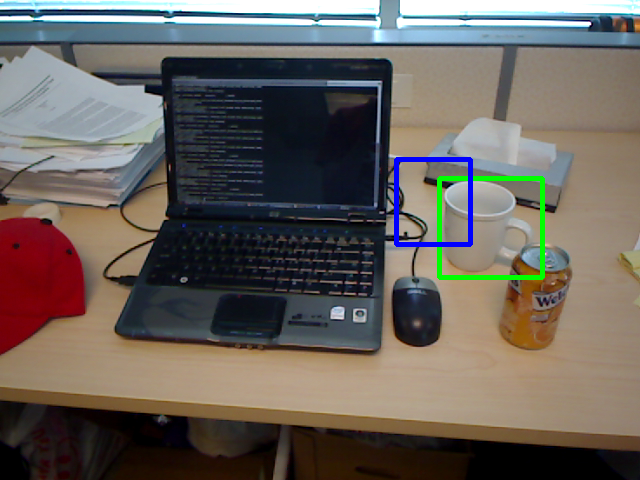
\includegraphics[width=\textwidth]{img/seguimiento_frame_template/frame_template-desk_1-coffee_mug_5-frame_27.png}
	\end{subfigure}
	\begin{subfigure}[b]{0.3\textwidth}
		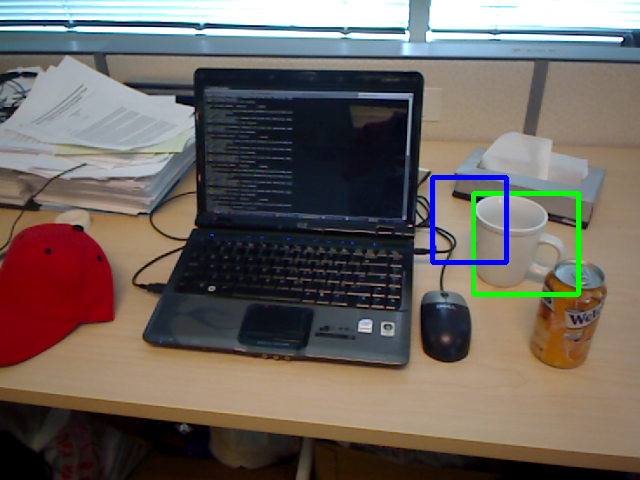
\includegraphics[width=\textwidth]{img/seguimiento_frame_template/frame_template-desk_1-coffee_mug_5-frame_28.png}
	\end{subfigure}


	\begin{subfigure}[b]{0.3\textwidth}
		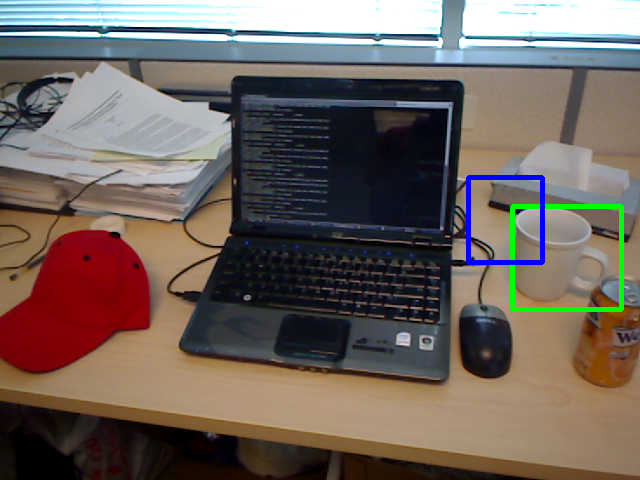
\includegraphics[width=\textwidth]{img/seguimiento_frame_template/frame_template-desk_1-coffee_mug_5-frame_29.png}
	\end{subfigure}
	\begin{subfigure}[b]{0.3\textwidth}
		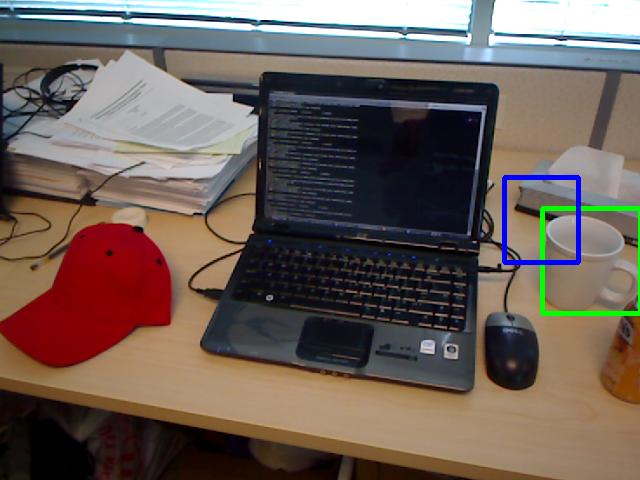
\includegraphics[width=\textwidth]{img/seguimiento_frame_template/frame_template-desk_1-coffee_mug_5-frame_30.png}
	\end{subfigure}
	\begin{subfigure}[b]{0.3\textwidth}
		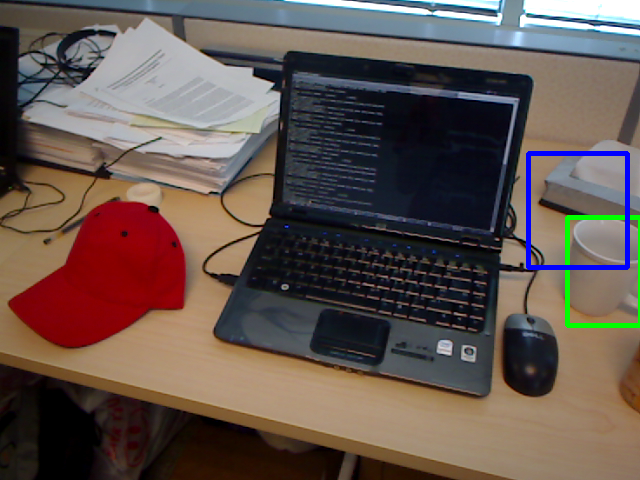
\includegraphics[width=\textwidth]{img/seguimiento_frame_template/frame_template-desk_1-coffee_mug_5-frame_31.png}
	\end{subfigure}

	\begin{subfigure}[b]{0.3\textwidth}
		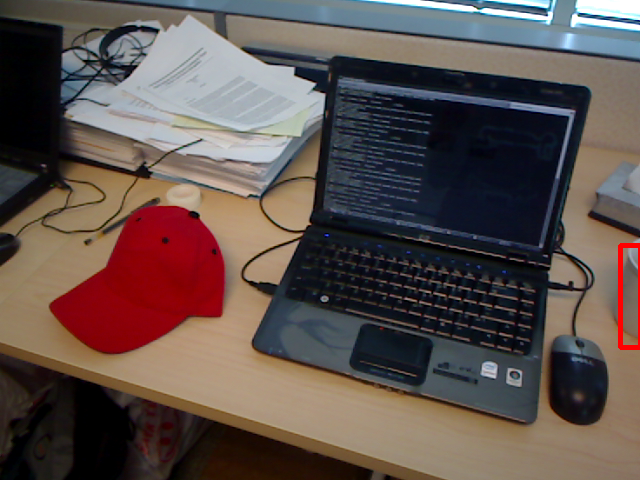
\includegraphics[width=\textwidth]{img/seguimiento_frame_template/frame_template-desk_1-coffee_mug_5-frame_32.png}
	\end{subfigure}
	\begin{subfigure}[b]{0.3\textwidth}
		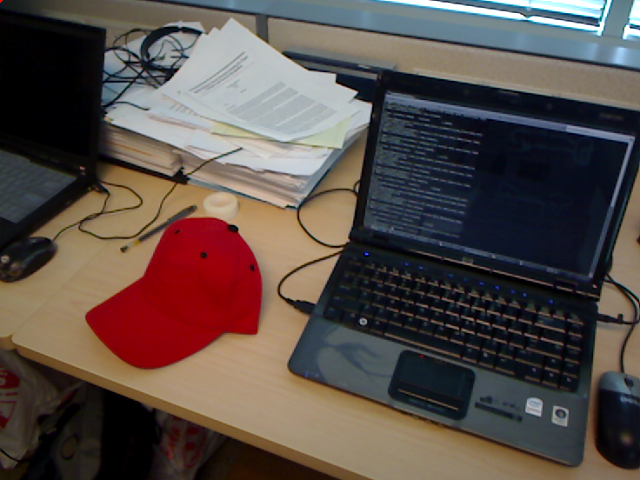
\includegraphics[width=\textwidth]{img/seguimiento_frame_template/frame_template-desk_1-coffee_mug_5-frame_33.png}
	\end{subfigure}
	\begin{subfigure}[b]{0.3\textwidth}
		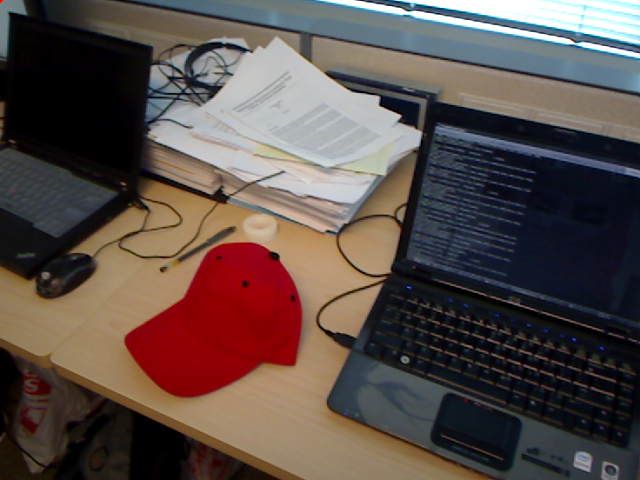
\includegraphics[width=\textwidth]{img/seguimiento_frame_template/frame_template-desk_1-coffee_mug_5-frame_34.png}
	\end{subfigure}

	\caption{Seguimiento frame a frame sin falsos positivos. Aquí se estaba usando las comparaciones de histogramas entre el frame anterior, el actual y el template del objeto}
	\label{frame_template_tracking}
\end{figure}

Una vez corridas estas dos sub-etapas dentro de la etapa de seguimiento, pueden ocurrir dos cosas. Una es si el algoritmo reportó haber encontrado al objeto. En este caso se almacenan los datos necesarios y se continúa utilizando el algoritmo de seguimiento en el frame siguiente. Si en cambio el algoritmo indica que el objeto no se encontró, se vuelve a la etapa de detección explicada previamente.



\section{Método propuesto en D}
\subsection{Alignment prerejective}\label{alignment_prerejective}
En esta sección explicaremos el método de estimación de pose proveniente del trabajo \cite{6630856}, el cual fue utilizado en gran parte de este trabajo.

El problema de determinar una transformación que permita alinear dos superficies ha generado muchas investigaciones en el campo de la visión en computación. Desde la manipulación de objetos en robótica hasta la reconstrucción de un modelo de un objeto o escena a partir de varias imágenes tomadas de distintos ángulos. En general estos métodos requieren una solución precisa para luego poder utilizar el resultado con otros problemas de procesamiento.

Hay muchos métodos conocidos para resolver este problema tanto en el dominio 2D como en el 3D y en general están basados en extracción de descriptores para eliminar falsas correspondencias entre las dos superficies o modelos. Es ampliamente conocido el hecho que los descriptores locales proveen una alta estabilidad dada su tolerancia al ruido y ocluciones. El objetivo de este trabajo era combinar inputs de ambos dominios de manera eficiente para resolver el problema de la estimación de pose.

En este trabajo realizan una serie de pasos bien definida hasta obtener una transformación como resultado final que indique la pose del objeto en la escena. En primer instancia, se obtienen puntos de interés utilizando un sistema ECV (\textit{Early Cognitive Vision}) cuya densidad está en un punto intermedio entre una imagen con puntos de interés escasos y descriptores de formas en 3D muy densos. Este sistema permite clasificar regiones de una imagen en tres categorías: región homogenea, región de borde y región con textura. En este trabajo se usan solo las últimas dos categorías ya que los pixeles en las regiones homogeneas resultan ser ambiguos para buscar correspondencias. Luego le agregan a cada descriptor información de sus vecinos, tanto de texturas como de formas, para aumentar la habilidad del método para distinguir falsas correspondencias. A esto lo llaman \textit{ECV context descriptors}.

Una vez recolectada esta información, utilizan \textit{RANSAC} para estimar una transformación que alinee el objeto con la escena. Formalmente lo que se busca es una transformación que minimice la suma de la diferencia de cuadrados entre los puntos del modelo y sus correspondencias en la escena. Para lograr esto se realizan los siguientes pasos:
\begin{enumerate}
	\item Tomar 3 o más puntos del objeto y sus correspondencias en la escena usando los descriptores de contexto ECV
	\item Estimar una transformacion usando esas correspondencias
	\item Aplicar la transformación al objeto
	\item Buscar \textit{inliers} usando búsqueda de vecinos cercanos entre el objeto transformado y la escena. Si el número de inliers es bajo, volver al primer paso
	\item Medir la diferencia de cuadrados usando los inliers y si es el menor valor encontrado guardar la transformación como resultado
\end{enumerate}

Esto puede repetirse durante las iteraciones que se pretendan o cuando la diferencia de cuadrados sea menor que un umbral dado. En este trabajo se agrega un paso novedoso a este esquema RANSAC enumerado previamente. Este paso asume una propiedad geométrica de objetos rígidos para descartar rápidamente malas correspondencias. En particular utilizan el hecho que las distancias se mantienen y hacen un chequeo de las diferencias entre las distancias de los bordes del polígono virtual formado por los puntos random tomados en el paso 1 tanto para el objeto como para la escena. Utilizando una medida de distancia entre estos valores y un umbral descartan rápidamente malas correspondencias. Si se asume que no se descartan potenciales poses que alinean bien los modelos, se obtiene la misma probabilidad de éxito de manera mucho más rápida.


\subsection{Iterative Closest Point (ICP)}\label{ICP}


\subsection{Entrenamiento}
Para esta primera etapa existen varias posibilidades distintas que van desde utilizar una única nube de puntos hasta generar un modelo completo del objeto 3D alineando todas las nubes de puntos disponibles en la base. Durante las pruebas preeliminares realizadas los algoritmos respondieron bien utilizando una única nube de puntos como modelo del objeto. Este motivo sumado a que en este trabajo nuestro objetivo se enfocó en la etapa de tracking, nos llevaron a optar por utilizar una única nube de puntos del objeto como modelo. Además pensando en términos prácticos, es mucho más factible obtener rápidamente una única nube de puntos del objeto que deseamos seguir a obtener un modelo completo 3D del mismo.

En el caso de estudio de esta tesis, la nube de puntos del objeto a seguir se obtuvo de la base de datos explicada en el capítulo \ref{base_rgbd}. De manera similar al entrenamiento en RGB, se tomó como nube de puntos modelo del objeto a la nube proveniente de la imágen de rotación 0 de una de las escenas del objeto. Una vez almacenados estos datos, se continúa con la siguiente etapa que es la de detección.

\comentarioP{Relacionar con template matching}

\subsection{Detección}
Para esta segunda etapa se utilizó el método descripto en la sección \ref{alignment_prerejective} refinando el resultado con ICP. La elección del mismo se realizó luego de correr varias pruebas que corroboraran la factibilidad del mismo. En estas pruebas también se observó que si la región donde se buscaba el objeto era lo suficientemente pequeña la búsqueda era más robusta.\comentarioP{Mejor más chica?} Teniendo en cuenta esto se pensó en una variante para la detección que utilice el método elegido. Esta tiene como primer paso obtener el alto y el ancho del modelo del objeto a seguir y escalarlos. Considerando cada una de estas escalas, dividimos la escena en cuadrantes de ese tamaño y corrimos el método de detección en cada cuadrante. Con el fin de detectar el objeto cuando el mismo se extiende sobre dos o más regiones, la búsqueda se hizo utilizando un marco que recorre todos los cuadrantes y sus uniones, como puede observarse en la figura \ref{frames_solapados}. Notar que la división por cuadrantes solo se realizó en los ejes ``x'' e ``y'' y no en el eje ``z'' ya que las pruebas preeliminares dieron buenos resultados de esta manera. La detección se corre en cada uno de estos cuadrantes y puede suceder que:
\begin{itemize}
	\item No se encontró el objeto en ningún cuadrante: en este caso el algoritmo indica que el objeto no se encuentra en el frame
	\item Se encontró el objeto en un cuadrante
	\item Se encontró el objeto en varios cuadrantes: el algoritmo devuelve la mejor posición encontrada según un puntaje de buena alineación devuelto por el algoritmo \ap.
\end{itemize}

Si la detección es positiva, se refina la alineación corriendo ICP entre el modelo del objeto transformado por el método ``alignment prerejective'' y el cuadrante de la escena donde fue encontrado el mismo. Con el objetivo de comenzar el seguimiento en las mejores condiciones posibles, se intentan tomar los puntos del objeto buscado pertenecientes a la escena. Esto se realiza porque se asume que el objeto se va modificando cuadro a cuadro, ya sea por movimientos de la cámara o del objeto. Una de las formas para obtener los puntos del modelo del objeto en la escena es utilizando un \kdt\footnote{AGREGAR REFERENCIA A KDTREE}. \comentarioP{Explicar un poco que es un kdtree} Se arma un \kdt con los puntos provenientes del modelo alineado y se filtran uno a uno los puntos de la escena que se encuentren cerca de al menos un punto del modelo en un cierto radio de distancia. \comentarioM{Explicar el ajuste automatico del LEAF} Los puntos que surjan de esta búsqueda son los considerados como encontrados en la escena. Para que el algoritmo de búsqueda considere exitosa la detección, la cantidad de puntos filtrados de la escena debe ser mayor o igual al 50\% de los puntos del modelo original. Si todas estas etapas son superadas con éxito, se considera que el objeto fue encontrado y se pasa a la siguiente etapa de seguimiento. Si cualquiera de estos pasos fallara, se comienza nuevamente con la etapa de detección en el siguiente frame.


\subsection{Seguimiento (ex Método de seguimiento en profundidad)}
El método de seguimiento elegido para profundidad es ICP, explicado en la sección \ref{ICP}. En esta sección explicaremos cómo fue la selección de los parámetros para este método y los resultados obtenidos con los parámetros elegidos.

La implementación de ICP utilizada es la incluida en la librería ``Point Cloud Library'' \cite{Rusu_ICRA2011_PCL}. Esta implementación admite distintos parámetros para modificar el comportamiento del método. Los parámetros explorados son los siguientes:

\begin{enumerate}
	\item Distancia máxima de correspondencia: Si entre dos puntos existe una distancia mayor a este valor no se van a tener en cuenta para la búsqueda de correspondencias.
	\item Número de iteraciones máximo: Criterio de corte.
	\item Distancia mínima entre transformaciones: Criterio de corte. Si dos transformaciones consecutivas tienen una distancia menor a este valor, el algoritmo termina.
	\item Suma euclidea mínima: Criterio de corte. Es la diferencia euclidea mínima permitida entre dos pasos del algoritmo.
\end{enumerate}

Además, una vez que converge ICP la librería facilita el valor de la suma del cuadrado de las distancias de la nube de puntos inicial a la nube de puntos destino como medida de que tan buena es la alineación obtenida. Este valor se utiliza como umbral para decidir si la respuesta encontrada se considera correcta o no, por lo que también se explora como el resto de los parámetros. A modo de refinar aún más el resultado, una vez hallada una buena alineación se procede a tomar los puntos de la escena que suponen ser los del objeto que se estaba buscando. La explicación de cómo se realiza este filtrado se puede ver en \comentarioM{EXPLICACION USO DE KDTREE. EXPLICAR EL AUTOAJUSTE DEL LEAF PARA KDTREE}. Una vez filtrados los puntos de la escena se compara esta cantidad de puntos con la cantidad de puntos que tiene el modelo del objeto. Si los puntos de la escena superan un porcentaje de puntos del modelo se considera que el objeto fue encontrado. Este porcentaje también es uno de los parámetros explorados.


\section{Método propuesto en RGB-D}\label{metodo_rgbd}

\subsection{Entrenamiento}

\subsection{Detección}

\subsection{Seguimiento}\label{tracking_rgbd}










\chapter{Base de datos RGB-D}\label{base_rgbd}
Durante el desarrollo de este trabajo se utilizaron secuencias con información de \textit{ground truth} de imágenes RGB-D con el objetivo de aplicar los métodos estudiados y tener una referencia para hacer comparaciones y sacar conclusiones sobre su eficacia. Las escenas fueron tomados del trabajo de Kevin Lai et al. \cite{lai2011large} en donde se creó una base de objetos y escenas. Esta base cuenta con 20 escenas y cada una de ellas contiene entre 100 y 200 frames RGB-D. El ground truth de esta base provee información frame a frame de qué objetos aparecen y cuál es su ubicación en el plano XY.

{\huge Figura con ejemplos de las escenas, por ejemplo: 2 filas con varias columnas cada una en donde haya frames RGB arriba y sus equivalentes en depth abajo}

Por otra parte, la base provee imágenes RGB-D de los objetos presentes en las escenas capturadas aisladamente con el objetivo de obtener su representación 3D.\comentarioP{Comentar como fueron adquiridas la resolución, longitud y ¿?} Cada una de estas imágenes es acompañada además por una máscara que segmenta al objeto buscado y la información de profundidad (nube de puntos) del objeto. Para tomar estas imágenes los objetos fueron ubicados en una base circular giratoria y, manteniendo la cámara en una posición fija, se tomaron muestras con cierta regularidad cubriendo toda la circunferencia de cada objeto. Esto se hizo además desde distintas alturas permitiendo apreciar la profundidad del objeto y así obtener una mejor descripción del mismo.

Los objetos elegidos para esta base se organizaron de una manera jerárquica tomada de las relaciones hiperónimo/hipónimo de WordNet. Cada objeto pertenece a una clase de objetos y hay varias instancias por cada clase. Por ejemplo, en la categoría ``taza'' existen varias instancias diferentes, que se corresponden simplemente a distintas tazas ya sea por forma o por color.

Existen distintas escenas que contienen a los objetos mencionados y en cada escena se combinan distintas clases de objetos y distintas instancias de la misma clase. De esta manera la base otorga la posibilidad de verificar algoritmos capaces de identificar instancias de objetos particulares o familias de objetos según la clasificación antes mencionada. En esta tesis usaremos .....


\chapter{Resultados y análisis}\label{chap:resultados}
En este capítulo se explican las pruebas realizadas durante el desarrollo de este trabajo a la vez que se analizan los resultados y se hacen hipótesis sobre los valores obtenidos. Se analizan todos los métodos explicados en el capítulo \ref{chap:sistema_de_seguimiento} por separado y se los compara entre sí hasta finalmente obtener de manera objetiva el mejor método de seguimiento.

Con el objetivo de elegir los métodos usados en cada etapa de cada sistema de seguimiento se realizaron varias pruebas. En este capítulo explicaremos cuales fueron estas pruebas, cómo se eligieron los valores para los distintos parámetros de cada método y mostraremos los resultados de los métodos elegidos, tanto para RGB como para profundidad. También analizaremos el funcionamiento del sistema de seguimiento RGB-D.

La experimentación realizada es rigurosa. Siguiendo el enfoque presente durante todo este trabajo, se corrieron y analizaron diversas pruebas para cada uno de los métodos de cada sistema por separado buscando los parámetros que mejor generalizaran el comportamiento deseado para los algoritmos. Por este motivo se realizaron pruebas para el seguimiento RGB por un lado, para profundidad por otro y una vez elegidos los parámetros, se analizaron los resultados para la unión de los métodos en el sistema de seguimiento RGB-D.

Para lograr una buena comparación entre métodos de seguimiento cuadro a cuadro, tanto para RGB como para profundidad, utilizamos como método de detección el método ``ideal''. El mismo consta simplemente de tomar los datos provistos por el \textit{ground truth} para los frames en donde se requería correr una detección. En el caso de RGB los datos son tomados directamente desde el ground truth. Como la base de datos solo provee la ubicación del objeto en RGB en el caso de la detección en profundidad estos datos se toman como punto de partida y luego se los refina tomando los datos del modelo 3D del objeto a buscar.

\section{Elección del método de seguimiento RGB}\label{sec:eleccion_rgb}
Durante el proceso de selección de métodos, se corrieron pruebas preliminares para elegir aquellos que mejor se adaptaran a las escenas y objetos representativos elegidos. Los objetos y escenas utilizados para este fin son los siguientes:
\begin{itemize}
	\item Taza, que aparece en la escena desk\_1
	\item Gorra, también en la escena desk\_1
	\item Bowl, que aparece en la escena desk\_2
\end{itemize}

Estos objetos y escenas son los que aparecen en las figuras \ref{fig:ejemplo_objetos_base} y \ref{fig:ejemplo_escenas_base}, tomados de la base de datos explicada en la Sección \ref{base_rgbd}.

Una vez hecho un primer filtro, se exploraron algunos parámetros de cada método para obtener los mejores valores de cada uno y luego hacer una selección final entre aquellos que mejor se desempeñaran. En esta sección explicaremos cuales fueron los métodos y cómo llegamos a elegir el definitivo.

Para el seguimiento RGB se tuvieron en cuenta dos métodos distintos. El primero utiliza SURF \cite{surf} para obtener puntos de interés y descriptores y luego un comparador para hacer comparaciones cuadro a cuadro. El segundo método consiste en extraer el histograma de la imagen RGB y utilizar una métrica para comparar histogramas para hacer el seguimiento.

El método que mejor se desempeñó en las pruebas preliminares es el basado en histogramas por lo que se exploraron distintas soluciones basadas en este método utilizando las escenas antes mencionadas. Este método tiene distintas variables a explorar:
\begin{itemize}
	\item Modelo de color: RGB o HSV y canales a utilizar de cada modelo
	\item Cantidad de categorías/celdas del histograma
	\item Método de comparación de histogramas: \textit{Bhattachayyra}, \textit{Chi-Squared}, \textit{Correlation}, \textit{Intersection}
	\item Umbrales para las distancias de los histogramas de los cuadrantes elegidos frame a frame y para la distancia de histogramas del template del objeto al cuadrante del frame en donde se busca
\end{itemize}


\begin{figure}
	\centering
	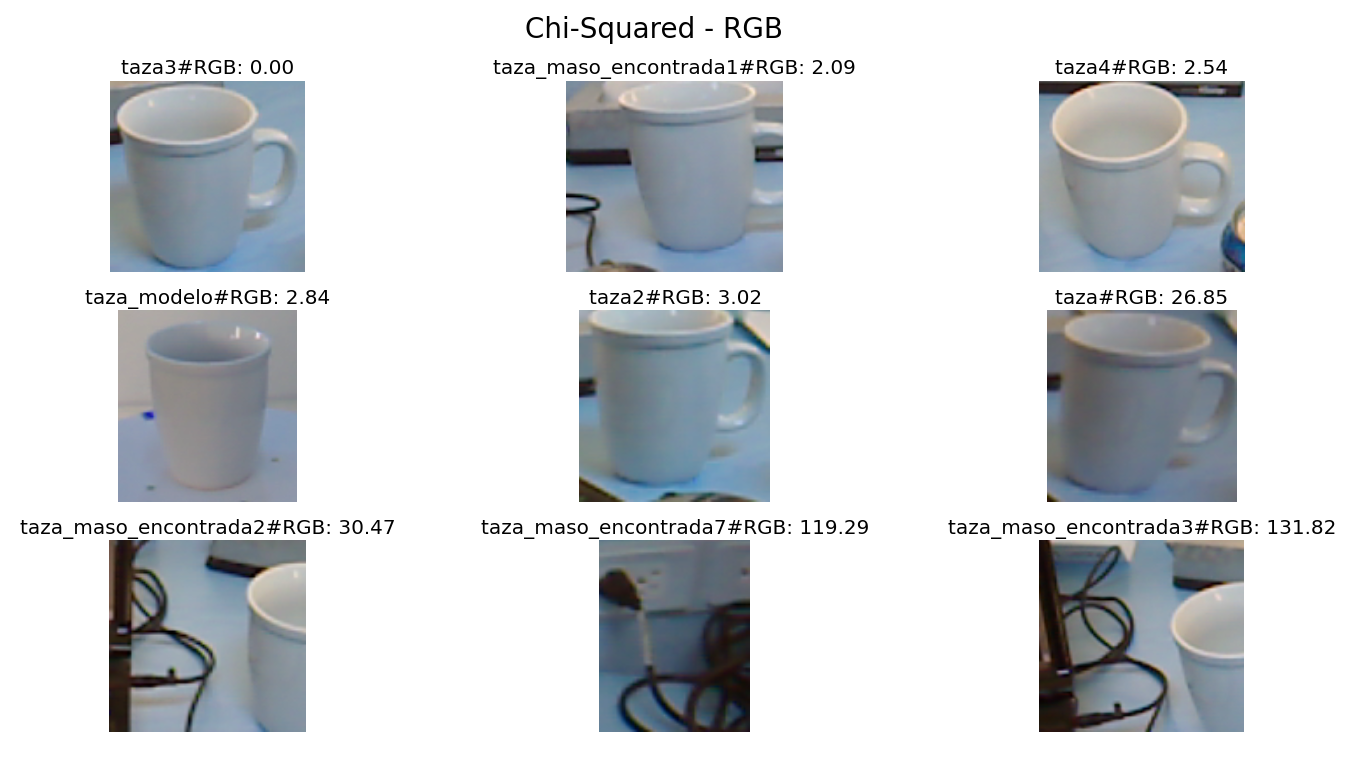
\includegraphics[width=\textwidth]{img/results_chi-squared_rgb_16r_4g_4b.png}
	\caption{Ordenando muestras según comparación por chi-squared, tomando los canales RGB, 16 bines para el canal rojo y 4 para el verde y el azul. El modelo utilizado es un template de la taza sacado de la escena.}
	\label{pruebas_eleccion_canales}
\end{figure}

Para decidir qué esquema de colores, qué canales y cuántas categorías por canal se iban a utilizar, se eligieron dos objetos representativos de la base con sus respectivas escenas y se tomaron muestras de cada uno junto con muestras de distintas texturas de la escena o del mismo objeto (en donde se lo veía de manera parcial).

Una vez tomadas las muestras se eligió una como template/modelo del objeto y se realizó una comparación entre el modelo y las distintas muestras tomadas de la escena y se ordenaron de menor a mayor distancia, fijando un método de comparación de histogramas, que también se evaluó. Un ejemplo de esto se puede ver en la Figura \ref{pruebas_eleccion_canales}. Esto se hizo con el objetivo de saber qué combinación de esquema, canales y bines por canal clasificaba mejor a las muestras.

\begin{equation}\label{eq:pascal_overlap}
Overlap(Area_A, Area_B) = \frac{Area_A \cap Area_B}{Area_A \cup Area_B - Area_A \cap Area_B}
\end{equation}


Para cuantificar la efectividad y robustes del tracking de cada algoritmo elegido decidimos evaluar las siguientes variables:
\begin{itemize}
	\item Porcentaje promedio de área solapada (\% promedio de overlap): promedio de solapamiento de área para todos los frames en donde se usó el algoritmo de seguimiento, usando el cálculo propuesto en \cite{everinghampascal}, entre la ubicación (\textit{bounding box} o caja de contorno) del objeto reportada por nuestro algoritmo y la reportada por el ground truth. La fórmula del cálculo es la presentada en la Ecuación \ref{eq:pascal_overlap}.
	\item Porcentaje de seguimiento: de todas las veces que el objeto aparece en la escena obtenemos el porcentaje de veces que el algoritmo de seguimiento fue exitoso, es decir que lo reporta como encontrado y el área reportada se solapa con el área reportada por el ground truth en al menos un 30\%\footnote{En la Sección \ref{sec:evaluacion_rgbd} se explica por qué se elige este valor.}
	\item Porcentaje de falsos positivos: cantidad de veces que el algoritmo reporta haber encontrado el objeto cuando en realidad no está en la imagen
	\item Porcentaje de falsos negativos: cantidad de veces que el algoritmo no encuentra el objeto cuando en realidad el mismo está en la imagen o que lo encuentra pero el área reportada se solapa en menos de un 30\% con el área reportada por el ground truth
\end{itemize}

Para realizar el cálculo de falsos positivos y falsos negativos se tuvo en cuenta la información frame a frame del ground truth así como también los resultados reportados por nuestro algoritmo.

De este análisis surgió que las mejores combinaciones de esquema, canales y bines para estos ejemplos fueron utilizar el canal verde en el caso de RGB con unos 60 bines, los 3 canales RGB con 8 bines por canal y los canales SV del esquema de colores HSV, con 8 y 16 bines respectivamente. Una vez reducido el espectro de posibilidades comenzamos a realizar pruebas con el fin de definir para cada uno de estos esquemas qué método de comparación de histogramas convenía utilizar y con qué valor de umbral se obtenian mejores resultados.

\begin{table}[h]
	\centering
	\begin{tabular}{|c|c|c|c|c|c|}
	    \hline
	    & \multirow{2}{2.4cm}{\% promedio de overlap} & \multirow{2}{2cm}{\% veces seguido} & \multirow{2}{1.6cm}{\% Falsos Positivos} & \multirow{2}{1.6cm}{\% Falsos Negativos}\\
		Objeto & & & &\\
	    \hline
	    Taza   & 19.30      & 26.32   & 0       & 46.94 \\
	    \hline
	    Gorra  & 49.10      & 87.80   & 0       & 0     \\
	    \hline
	    Bowl   & 14.14      &  4.55   & 0       & 20    \\
	    \hline
    \end{tabular}
	\caption{Mejores resultados usando comparación de histogramas por Bhattachayyra para el canal verde con 60 bines}
	\label{pruebas_definitivas_bhatta_green}
\end{table}

\begin{table}[h]
	\centering
	\begin{tabular}{|c|c|c|c|c|c|}
	    \hline
	    & \multirow{2}{2.4cm}{\% promedio de overlap} & \multirow{2}{2cm}{\% veces seguido} & \multirow{2}{1.6cm}{\% Falsos Positivos} & \multirow{2}{1.6cm}{\% Falsos Negativos}\\
		Objeto & & & &\\
	    \hline
	    Taza   & 14.83      & 13.16     & 0      & 58.16 \\
	    \hline
	    Gorra  & 49.14      & 95.12     & 0      & 1.02  \\
	    \hline
	    Bowl   & 17.47      & 13.64     & 5.26   & 26.84 \\
	    \hline
    \end{tabular}
	\caption{Mejores resultados usando comparación de histogramas por Correlation para el canal verde con 60 bines}
	\label{pruebas_definitivas_correl_green}
\end{table}

\begin{table}[h]
	\centering
	\begin{tabular}{|c|c|c|c|c|c|}
	    \hline
	    & \multirow{2}{2.4cm}{\% promedio de overlap} & \multirow{2}{2cm}{\% veces seguido} & \multirow{2}{1.6cm}{\% Falsos Positivos} & \multirow{2}{1.6cm}{\% Falsos Negativos}\\
		Objeto & & & &\\
	    \hline
	    Taza   & 34.48      & 47.89     & 0        & 31.63  \\
	    \hline
	    Gorra  & 55.68      & 96.97     & 0        & 0      \\
	    \hline
	    Bowl   & 12.58      &  6.19     & 0        & 13.68  \\
	    \hline
    \end{tabular}
	\caption{Mejores resultados combinando comparación de histogramas por Bhattachayyra para RGB y para SV (del esquema HSV)}
	\label{tab:tabla_rgb}
\end{table}

Los mejores resultados que obtuvimos se encuentran en las tablas \ref{pruebas_definitivas_bhatta_green}, \ref{pruebas_definitivas_correl_green} y \ref{tab:tabla_rgb}. Como se puede observar, el método de seguimiento utilizando la distancia de Bhattachayyra combinando los modelos RGB y HSV es el que mejor resultados arroja, superando a los otros métodos en el análisis de falsos positivos y falsos negativos, y en la mayoría de los ejemplos también supera en porcentaje de promedio de solapamiento (overlap) y de seguimiento.


\section{Evaluación del tracking RGB}\label{eval_rgb}
A continuación se muestran los resultados del algoritmo de seguimiento elegido para las imágenes RGB con los valores de los parámetros ya fijados. Para todas las pruebas se usaron los tres objetos, y las escenas donde aparecen, nombrados en la Sección \ref{sec:eleccion_rgb} sacados de la base de datos indicada en la Sección \ref{base_rgbd}.

Como podemos ver en la Tabla \ref{tab:tabla_rgb}, el tracking se comporta de manera muy diversa dependiendo del objeto que se esté analizando. En los ejemplos de la taza y la gorra el algoritmo reporta haber encontrado al objeto en la mayoría de los casos, 85\% y 78\% respectivamente. Este valor en conjunto con el promedio de solapamiento pueden darnos un indicio de que tan bien se desempeña el algoritmo.

Si observamos el promedio de solapamiento vemos que el algoritmo se comporta mucho mejor en el caso de la gorra, con un promedio de solapamiento del 55\%. Esto se debe a la marcada diferencia de color entre la gorra y el fondo de la imagen. Esto no sucede en el caso de la taza en el que repetidas veces el color de fondo varía entre colores y tonos similares a los de esta, lo que provoca que la comparación de histogramas no sea robusta. Este problema con las variaciones de colores del fondo es común en los métodos basados en histogramas.

En el caso del bowl el promedio de solapamiento es alto pero se debe a que el porcentaje de veces que se siguió al objeto es bajo. Como el algoritmo de detección es el ideal, cuantas más veces se usa la detección mejor es el porcentaje de solapamiento. Notamos que en esta escena los cambios de intensidad y textura son muy notorios lo que afecta negativamente al algoritmo.


\begin{figure}
	\centering
	\begin{subfigure}[b]{0.9\textwidth}
		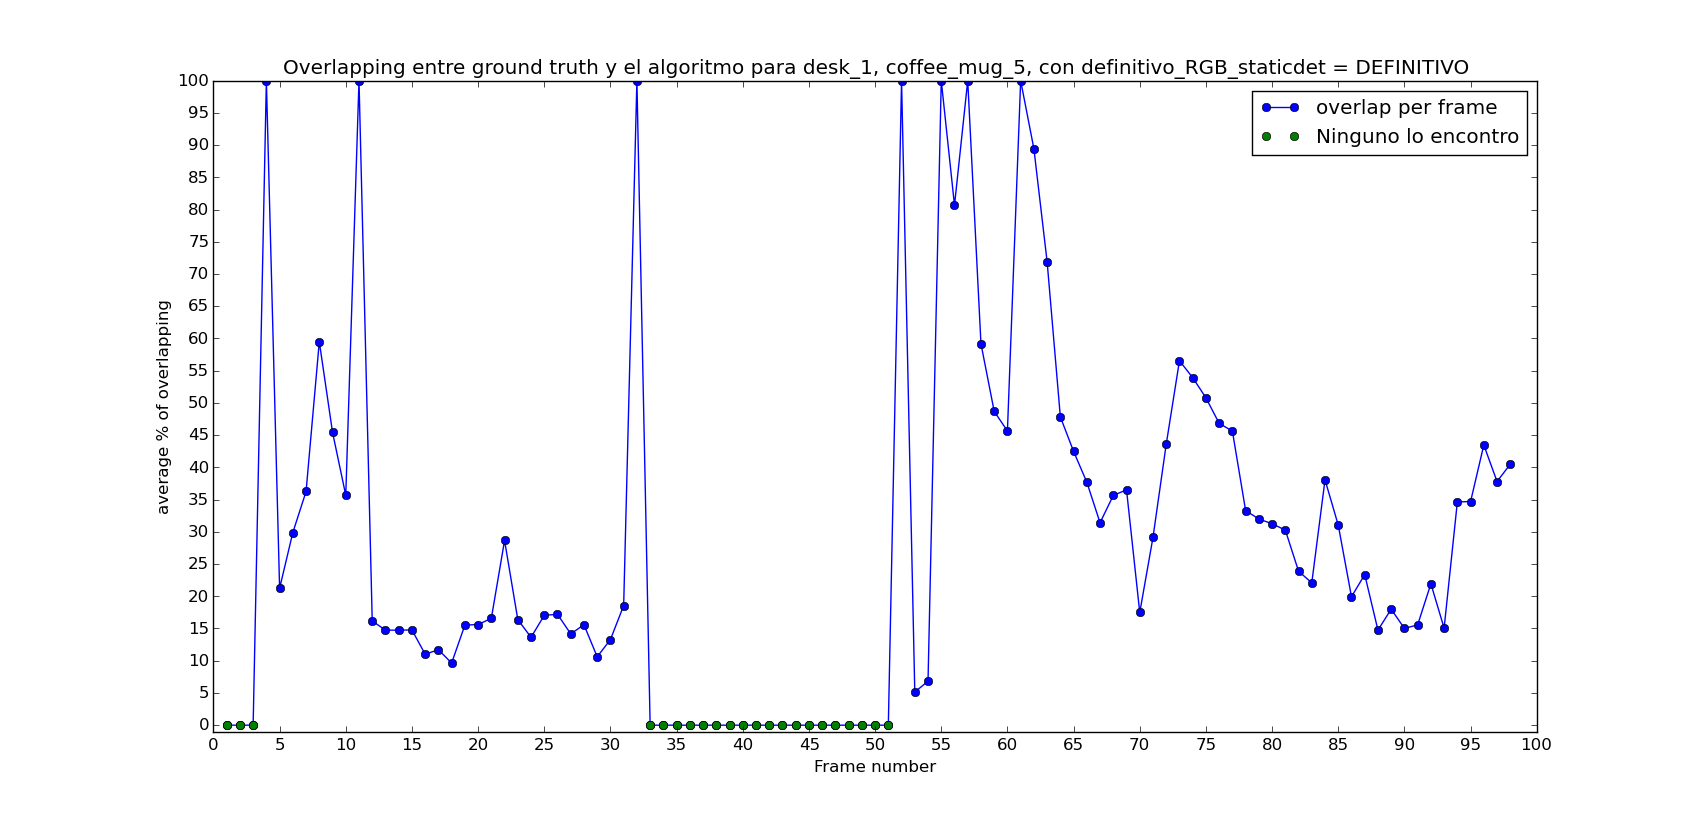
\includegraphics[width=\textwidth]{img/frame_a_frame/rgb-taza.png}
		\caption{Seguimiento frame a frame para la taza}
		\label{frame_frame_rgb_taza}
	\end{subfigure}
	\quad
	\begin{subfigure}[b]{0.9\textwidth}
		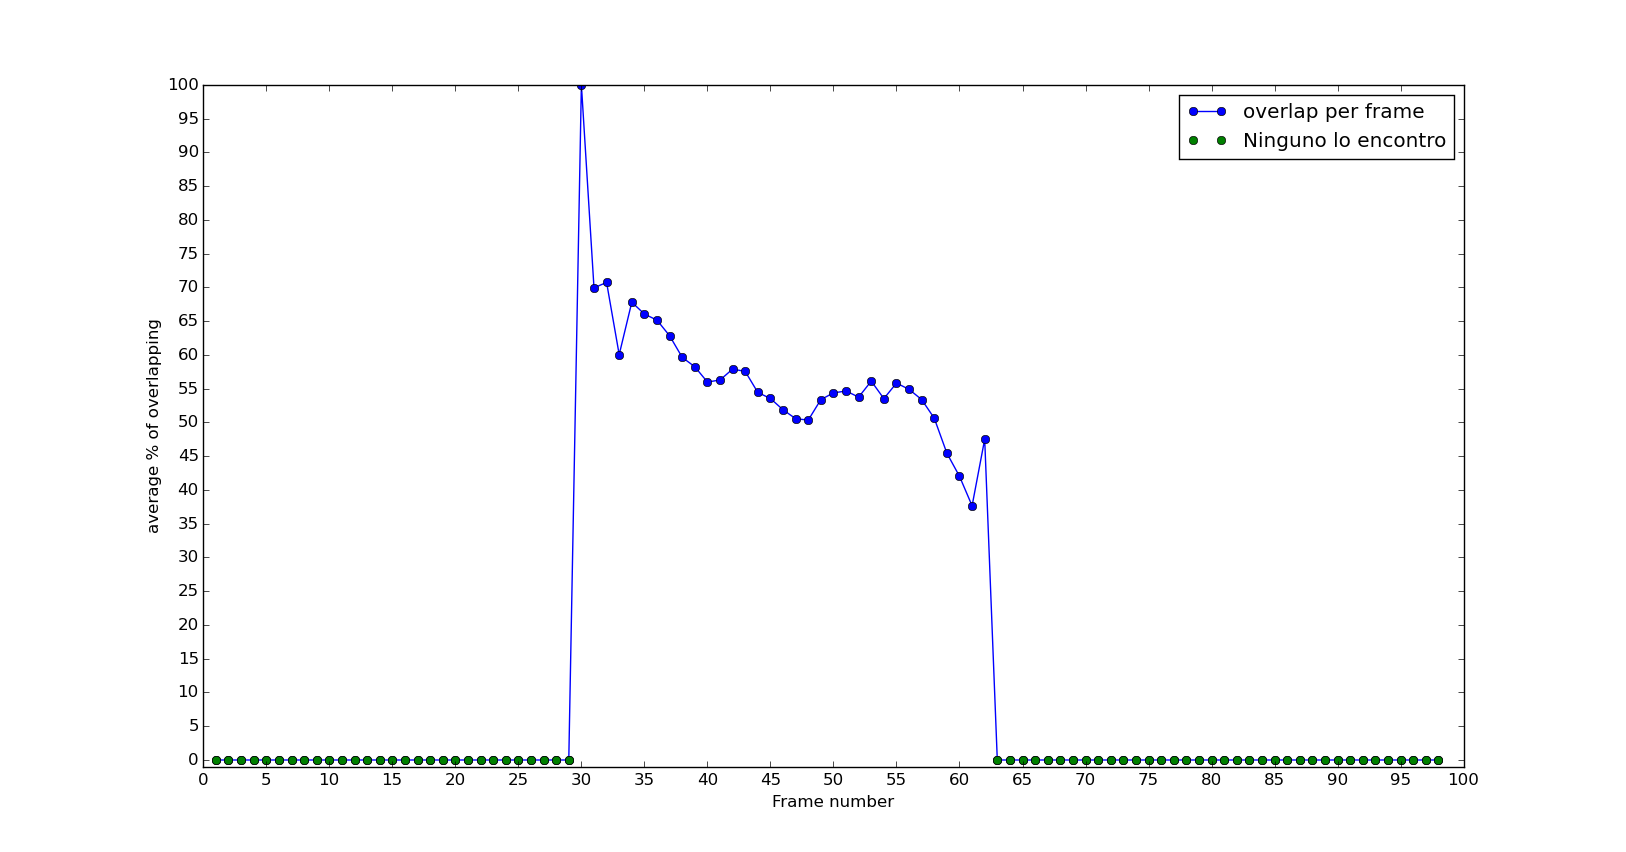
\includegraphics[width=\textwidth]{img/frame_a_frame/rgb-gorra.png}
		\caption{Seguimiento frame a frame para la gorra}
		\label{frame_frame_rgb_gorra}
	\end{subfigure}
	\quad
	\begin{subfigure}[b]{0.9\textwidth}
		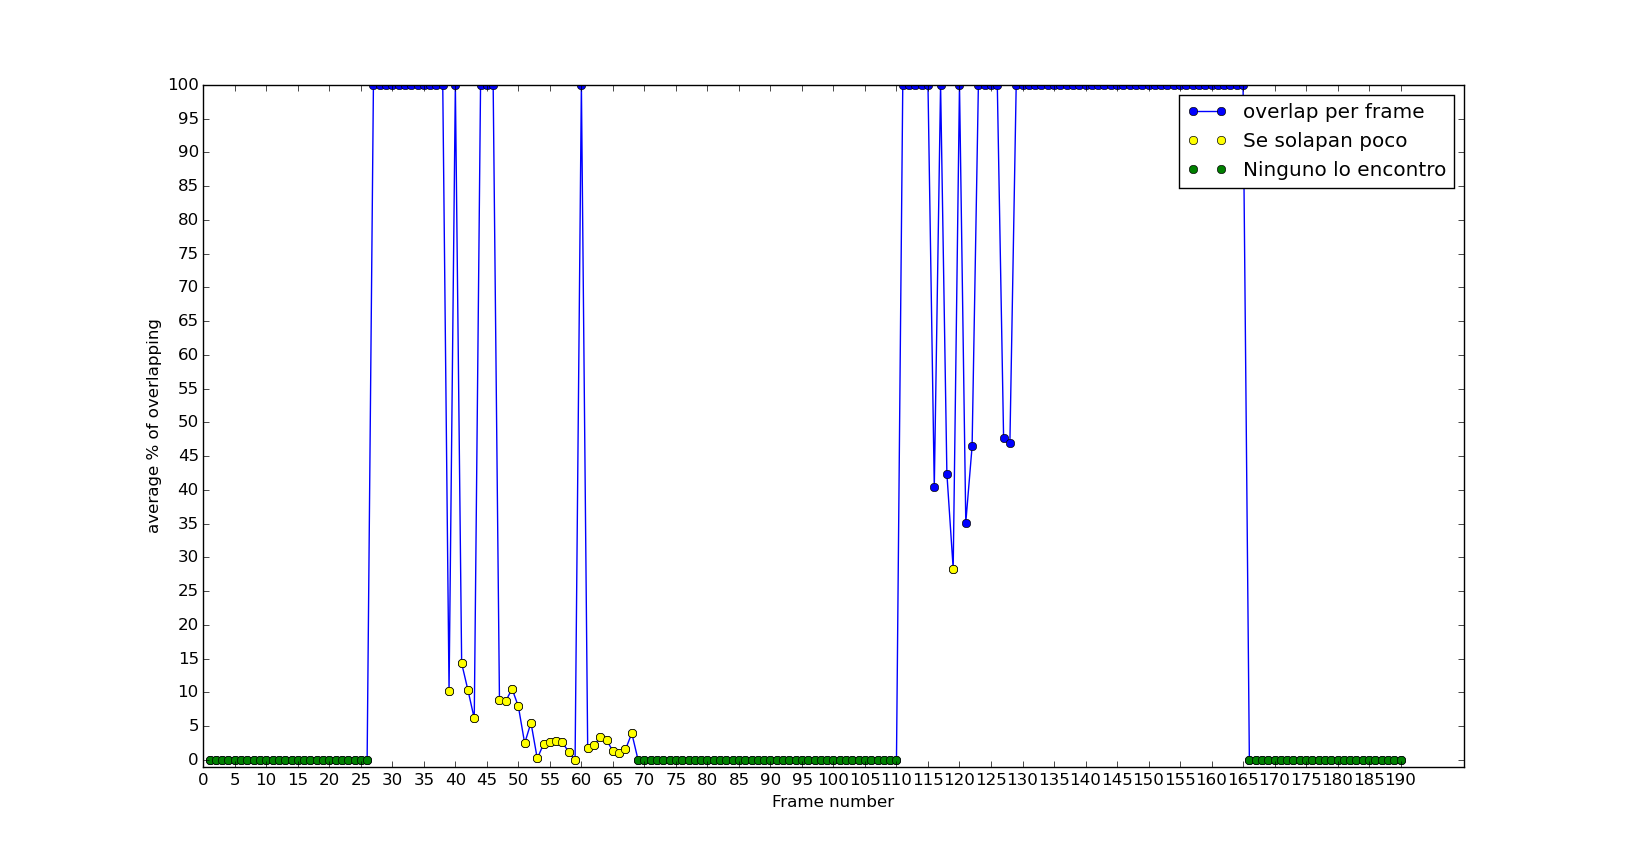
\includegraphics[width=\textwidth]{img/frame_a_frame/rgb-bowl.png}
		\caption{Seguimiento frame a frame para el bowl}
		\label{frame_frame_rgb_bowl}
	\end{subfigure}
	\caption{Seguimiento frame a frame del tracking RGB con detección ideal.}
	\label{frame_frame_rgb}
\end{figure}

En la Figura \ref{frame_frame_rgb} se visualiza mejor el comportamiento del algoritmo para cada objeto en las escenas ya nombradas (desk\_1 para la taza y la gorra, desk\_2 para el bowl). En cada subfigura se muestra para cada escena y por cada frame el porcentaje de solapamiento entre el área del objeto reportada por el algoritmo y la indicada por el ground truth, siguiendo la métrica de Pascal VOC \cite{everinghampascal}, dada por la Fórmula \ref{eq:pascal_overlap}.

\customsubsubsection{Colores en los gráficos de seguimiento frame a frame}
Los colores en los puntos del gráfico representan los distintos resultados registrados por cada frame.
\begin{itemize}
	\item Si el punto es de color verde, significa que el resultado reportado por nuestro algoritmo coincide con el ground truth en que el objeto no se encuentra en ese frame, es decir, es un verdadero negativo.
	\item Si el color es amarillo, significa que el algoritmo reportó haber encontrado al objeto y así también lo hace el ground truth, pero que las áreas reportadas no se solapan entre sí o el porcentaje de solapamiento es menor al 30\%. En este caso es un falso negativo.
	\item Si el punto es de color naranja, estamos frente a otro tipo de falso negativo. Este color se usa cuando nuestro algoritmo no reporta haber encontrado al objeto pero el ground truth indica que el obtejo está en el frame.
	\item El rojo indica un falso positivo, es decir, cuando el ground truth indica que el objeto no está en el frame y nuestro algoritmo reporta lo contrario.
	\item El color azul indica que el resultado reportado por nuestro algoritmo se solapa en un 30\% o más con el área indicada por el ground truth. A diferencia del resto de los colores antes mencionados que aparecen todos sobre el 0 del eje de porcentaje de solapamiento, los puntos azules pueden aparecer a cualquier nivel de este eje. La altura en donde esté el punto azul indica el porcentaje de solapamiento para ese frame.
	\item El negro solo aplica a los métodos de profundidad presentados. Este color se presenta cuando en distintas corridas del algoritmo para un objeto en una escena se obtienen dos resultados distintos para un mismo frame.
\end{itemize}

El motivo por el cual los puntos de color negro solo pueden aparecer en los resultados de los métodos de seguimiento en profundidad es que el método descripto en la Sección \ref{alignment_prerejective}, presente en estos métodos, utiliza RANSAC como esquema para obtener la estimación de pose. Una de las características de este tipo de esquemas es que la exploración se realiza de manera aleatoria. Esto provoca que dos corridas del algoritmo con mismos valores de entrada puedan diferir en el resultado, una indicando que se encontró una alineación y la otra que no. Para corroborar la robustes de nuestro algoritmo se lo ejecuta varias veces para cada valor de entrada y luego al momento de hacer este gráfico comparamos los valores que obtuvimos en cada corrida para cada frame. Si en todas las corridas se obtuvo el mismo resultado, es decir si se encontró o no se encontró el objeto, ese frame tiene un punto de algún color distinto al negro, entre los colores antes mencionados. Si en cambio hay distintos resultados entre las corridas, ese frame tendrá un punto de color negro y la altura del punto será el promedio del área solapada entre todas las corridas que tuvieron un resultado positivo para ese frame.


\customsubsubsection{Análisis del seguimiento frame a frame para RGB}
En la Figura \ref{frame_frame_rgb_taza} podemos ver que el algoritmo de seguimiento reporta un área que se solapa entre un 15\% y un 50\% en la mayoría de los casos. En la Figura \ref{frame_frame_rgb_gorra} la mayoría oscila entre un 35\% y un 50\% y en la Figura \ref{frame_frame_rgb_bowl} se observa que la mayoría se encuentra entre un 1\% y un 10\%. Una posible explicación de esto es que el algoritmo no funciona correctamente cuando los objetos tienen poca textura y esto empeora si existen objetos cercanos cuya textura sea similar a la del objeto que se está buscando. Este sería el caso de la taza y del bowl. Ambos son objetos con poca textura y de color blanco que pueden camuflarse con otros objetos de la escena.
Cabe aclarar que en las tres subfiguras antes mencionadas todos los frames cuyo área de solapamiento es igual a 100\% corresponden a aquellos frames en donde el tracking pierde el objeto y se utiliza al algoritmo de detección ideal para localizar al objeto nuevamente.

\section{Evaluación del tracking en profundidad}
En esta sección se muestran los resultados del tracking basado en ICP para las imágenes de profundidad descripto en la Sección \ref{tracking_rgbd} con los valores de los parámetros ya fijados. Para todas las pruebas se eligieron los mismos tres objetos que para el caso de la evaluación del tracking RGB (ver sección \ref{eval_rgb}).

\begin{table}[h]
	\centering
    \begin{tabular}{|c|c|c|c|c|c|}
    \hline
    & \multirow{2}{2.4cm}{\% promedio de overlap} & \multirow{2}{2cm}{\% veces seguido} & \multirow{2}{1.6cm}{\% Falsos Positivos} & \multirow{2}{1.6cm}{\% Falsos Negativos}\\
	Objeto & & & &\\
    \hline
    Taza   & 66.29      & 92.16      & 0      & 0     \\
    \hline
    Gorra  & 56.85      & 92.67      & 0      & 0     \\
    \hline
    Bowl   & 40.60      & 63.83      & 4.74   & 14.39 \\
    \hline
    \end{tabular}
\caption{Resultados del tracking en profundidad utilizando como detección los valores sacados de la base de datos más una etapa de refinamiento de estos datos usando los métodos explicados en las secciones \ref{alignment_prerejective} y \ref{ICP}}
\label{tabla_d}
\end{table}

En la Tabla \ref{tabla_d} se puede ver que el tracking se comporta de mejor manera que el algoritmo de RGB. Los tres ejemplos tienen una alta tasa de seguimiento. Además, en los tres casos se tiene un buen balance entre el promedio de solapamiento del área encontrada y el área reportada por el \textit{ground truth}.

\begin{figure}
	\centering
	\begin{subfigure}[b]{0.9\textwidth}
		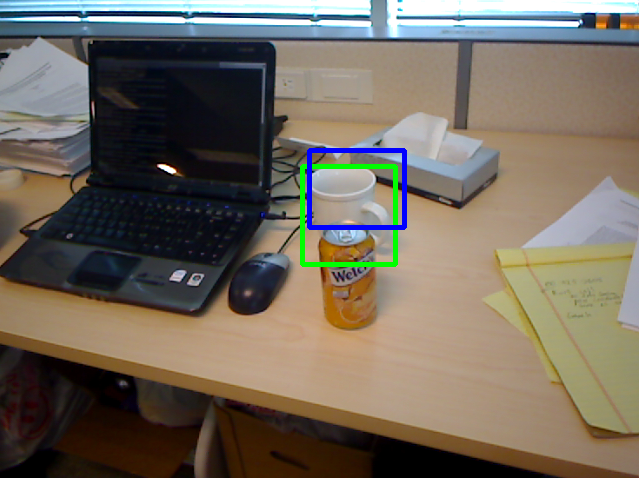
\includegraphics[width=\textwidth]{img/frame_98_taza_rgb.png}
		\caption{Seguimiento reportado por el tracking en profundidad y proyectado en RGB.}
		\label{taza_ocluida_rgb}
	\end{subfigure}
	\quad
	\begin{subfigure}[b]{0.9\textwidth}
		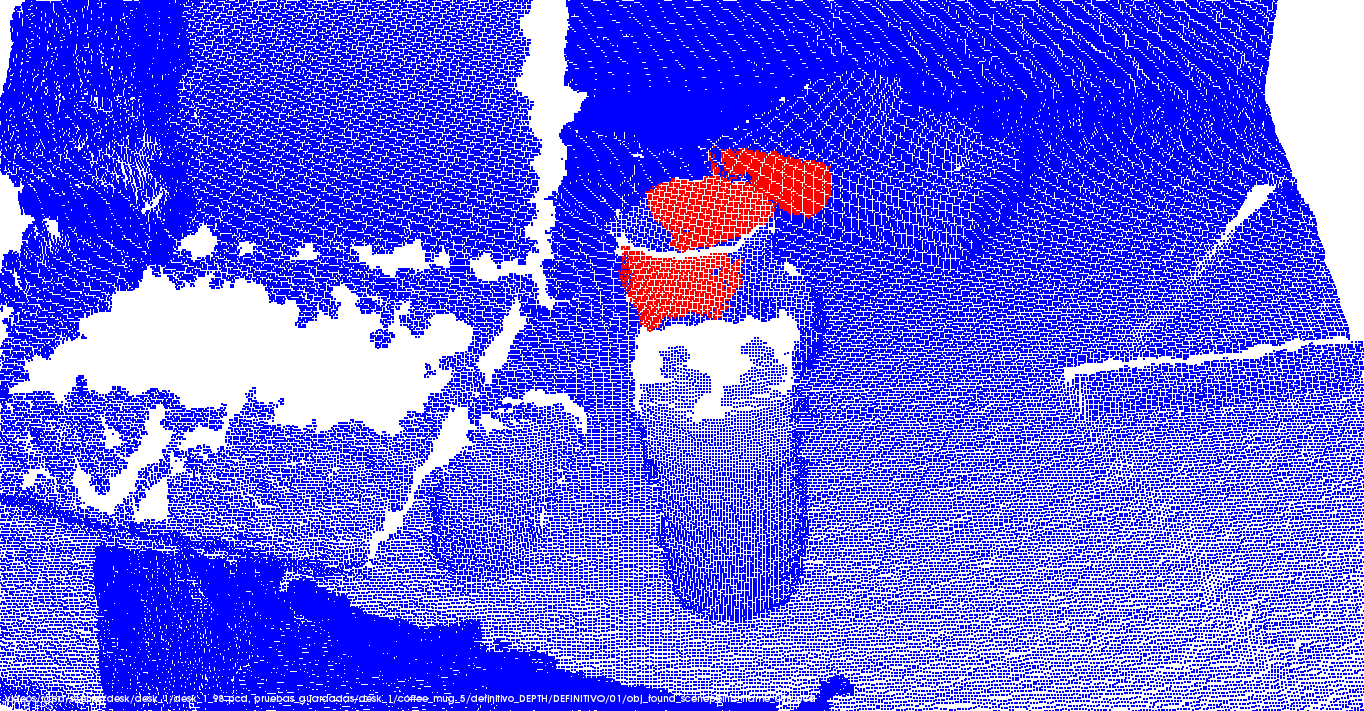
\includegraphics[width=\textwidth]{img/frame_98_taza_pcd.png}
		\caption{Visualización de la nube de puntos reportada por el tracking en profundidad}
		\label{taza_ocluida_pcd}
	\end{subfigure}
	\caption{Muestra de un resultado del seguimiento en profundidad. Las áreas se solapan en un 47\%.}
	\label{taza_ocluida}
\end{figure}

Un problema que encontramos en nuestra solución es que no hacemos un ajuste del tamaño del área reportada si el objeto está ocluído. En la Figura \ref{taza_ocluida} podemos ver como el algoritmo detecta de manera exitosa a la taza pero que solo reporta el área de la taza que está visible y no ajusta el tamaño al del modelo del objeto que se obtuvo en la etapa de entrenamiento. La subfigura \ref{taza_ocluida_rgb} muestra en color azul el recuadro reportado por nuestro algoritmo de seguimiento en donde se encuentra la taza. El recuadro verde corresponde al área que indica el ground truth como correcta. Se puede observar que el recuadro verde incluye además de la parte visible de la taza una porción importante de la lata que está delante de ella y que si se tiene en cuenta el tamaño de la taza esta área está incluyendo a la parte de la taza que se encuentra ocluida. A pesar de no ser algo que suceda reiteradas veces en las escenas y objetos elegidos para estas pruebas, puede ser un punto de mejora para nuestro algoritmo.

Otra decisión que se tomó al implementar nuestro algoritmo fue no utilizar el modelo del objeto para refinar el seguimiento, por ejemplo, para realizar el filtrado de puntos de la escena que corresponden al objeto que se busca. Esto se debe a que dependiendo de la forma del objeto, de su pose en el frame actual y de su pose en el modelo no resulta sencillo decidir si es conveniente utilizar el modelo para hacer este filtrado. En cambio, decidimos utilizar la nube de puntos hallada en el frame anterior como base para filtrar los puntos en el frame actual una vez que se quiera refinar el resultado. Por este motivo es que en ocaciones el algoritmo devuelve como parte del resultado puntos que no corresponden al objeto que se busca.

En la imagen \ref{taza_ocluida_pcd} se pueden ver tres regiones de puntos de color rojo. Esas regiones son las reportadas por el algoritmo como puntos de la taza. Si las enumeramos de arriba hacia abajo, la primera región no forma parte de la taza sino que es parte de la caja de pañuelos que está detrás de la misma. Esto podría evitarse si se filtraran los puntos de la escena usando el modelo de la taza pero sólo porque la forma de la misma es simétrica (si no se tiene en cuenta su asa). En el caso de la gorra en cambio ya no queda tan claro que sirva filtrar usando el modelo porque la visera la hace asimétrica y el tamaño de la misma no permite despreciar esos puntos.

Haciendo un análisis de los frames anteriores al de la Figura \ref{taza_ocluida} y de cómo se fue desarrollando el seguimiento notamos que el motivo por el cual se incluye parte de la caja de pañuelos como puntos de la taza es porque en la etapa de detección falló el refinamiento por AP e ICP y el filtrado de puntos (ver Sección \ref{subsec:deteccion_rgbd}). En la Figura \ref{filtro_en_deteccion} mostramos como se ve una detección sacada directa desde la base de datos (Subfigura \ref{filtro_en_deteccion_mal}) y un refinado de la detección (Subfigura \ref{filtro_en_deteccion_bien} utilizando el modelo del objeto y alineándolo usando AP e ICP y filtrando los puntos de la escena. Esto permite ver que una detección fallida o exitosa puede afectar a todo el seguimiento.

\begin{figure}
	\centering
	\begin{subfigure}[b]{0.9\textwidth}
		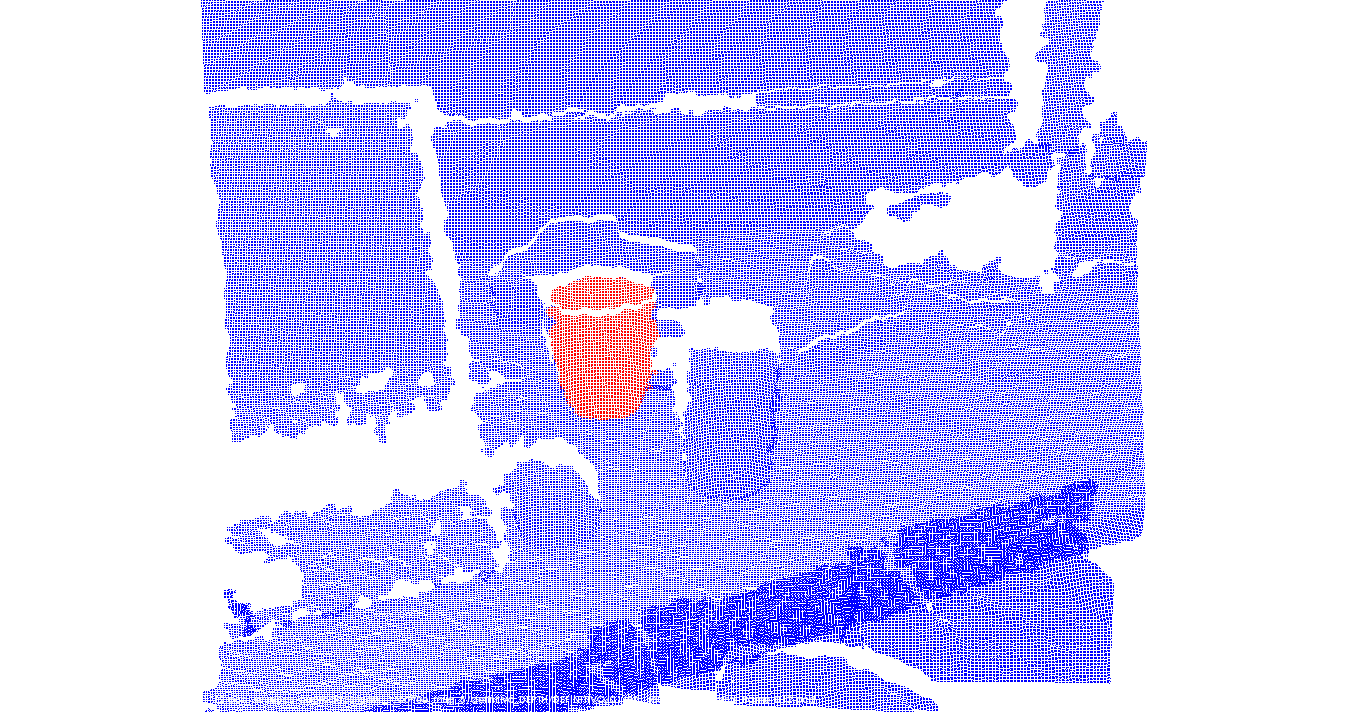
\includegraphics[width=\textwidth]{img/taza_filtrado_exitoso_definitivo_depth_frame12.png}
		\caption{Filtrado exitoso}
		\label{filtro_en_deteccion_bien}
	\end{subfigure}
	\quad
	\begin{subfigure}[b]{0.9\textwidth}
		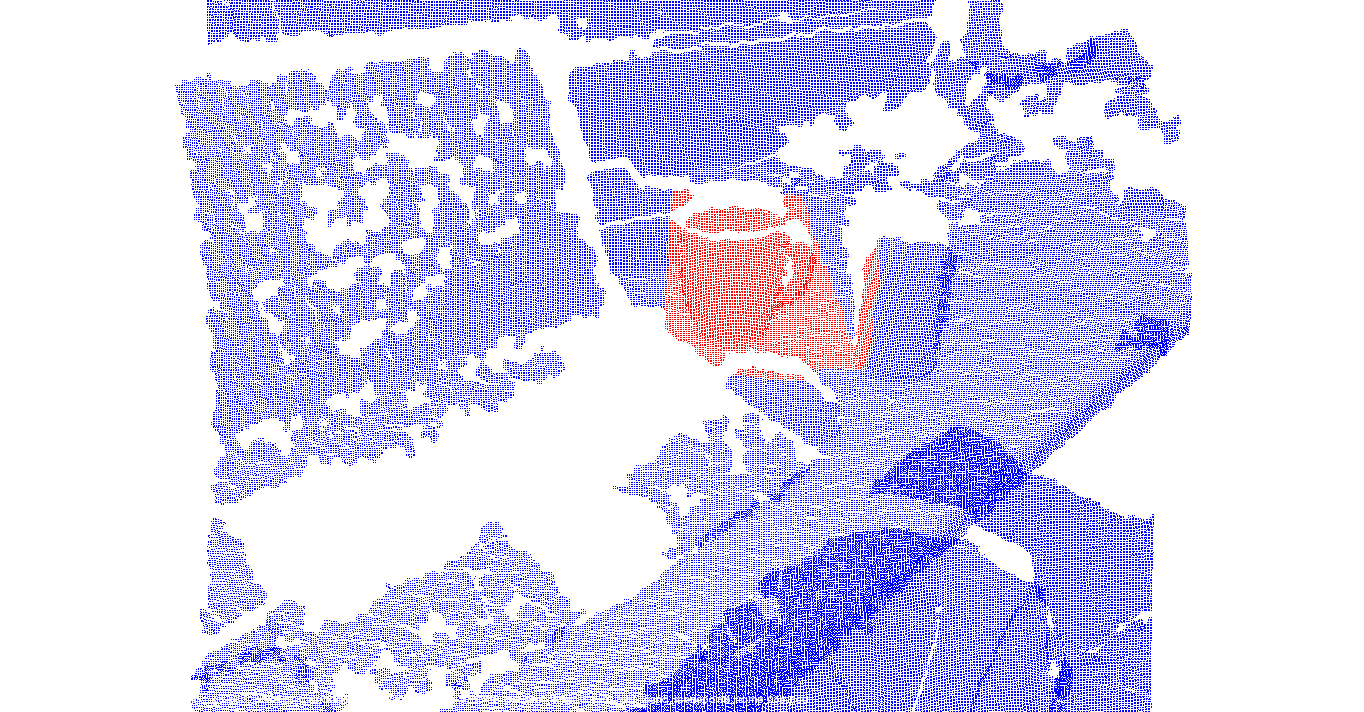
\includegraphics[width=\textwidth]{img/taza_filtrado_fallido_depth_simil_thresh_01_frame66.png}
		\caption{Filtrado fallido}
		\label{filtro_en_deteccion_mal}
	\end{subfigure}
	\caption{Nube de puntos de la taza filtrados de la escena}
	\label{filtro_en_deteccion}
\end{figure}

En la Figura \ref{frame_frame_d} se muestran para cada escena y objeto como se comportó el tracking frame a frame. El análisis es el mismo que se explicó para la Figura \ref{frame_frame_rgb}, aunque en estos gráficos aparecen algunas referencias nuevas.

En la Subfigura \ref{frame_frame_d_taza} se observan dos puntos de color naranja con valor 0\%. Estos valores corresponden a los frames 32 y 52 de la escena desk\_1 y son los dos falsos negativos reportados en la Tabla \ref{tabla_d} para la taza.

En la Figura \ref{frame_frame_d_gorra} se puede identificar un punto rojo correspondiente al frame 66 de la escena desk\_1 con un valor del 0\%. Este color indica que se produjo un falso positivo.

Por último, en la Figura \ref{frame_frame_d_bowl} existen múltiples puntos de color negro. Estos puntos indican que en las múltiples corridas del algoritmo para esta escena y con estos valores de parámetros hubo distintos resultados para el mismo frame (ver Sección \ref{eval_rgb}), indicando en este caso la falta de robustez del método. Entre los frames 72 y 108 el ground truth indica que el bowl no se encuentra en la escena. Los puntos negros en el gráfico \ref{frame_frame_d_bowl} entre dichos frames con valor 0\% indican que alguna de las corridas el algoritmo reportó haber encontrado al objeto, es decir que hubo falsos positivos y en otras reportó correctamente que el objeto no se hallaba en esos frames. Luego, entre los frames 109 y 122 además de haber puntos negros con valor 0\% existen algunos con valores mayormente cercanos al 15\%. Eso significa que en alguna de las corridas el algoritmo reportó haber encontrado al objeto y en otras no lo encontró en cuyo caso fueron falsos negativos.

Lo que buscamos con este análisis es reducir la cantidad de puntos negros al mínimo ya que es un indicador de que tan robusto es el algoritmo.

\begin{figure}
	\centering
	\begin{subfigure}[b]{0.9\textwidth}
		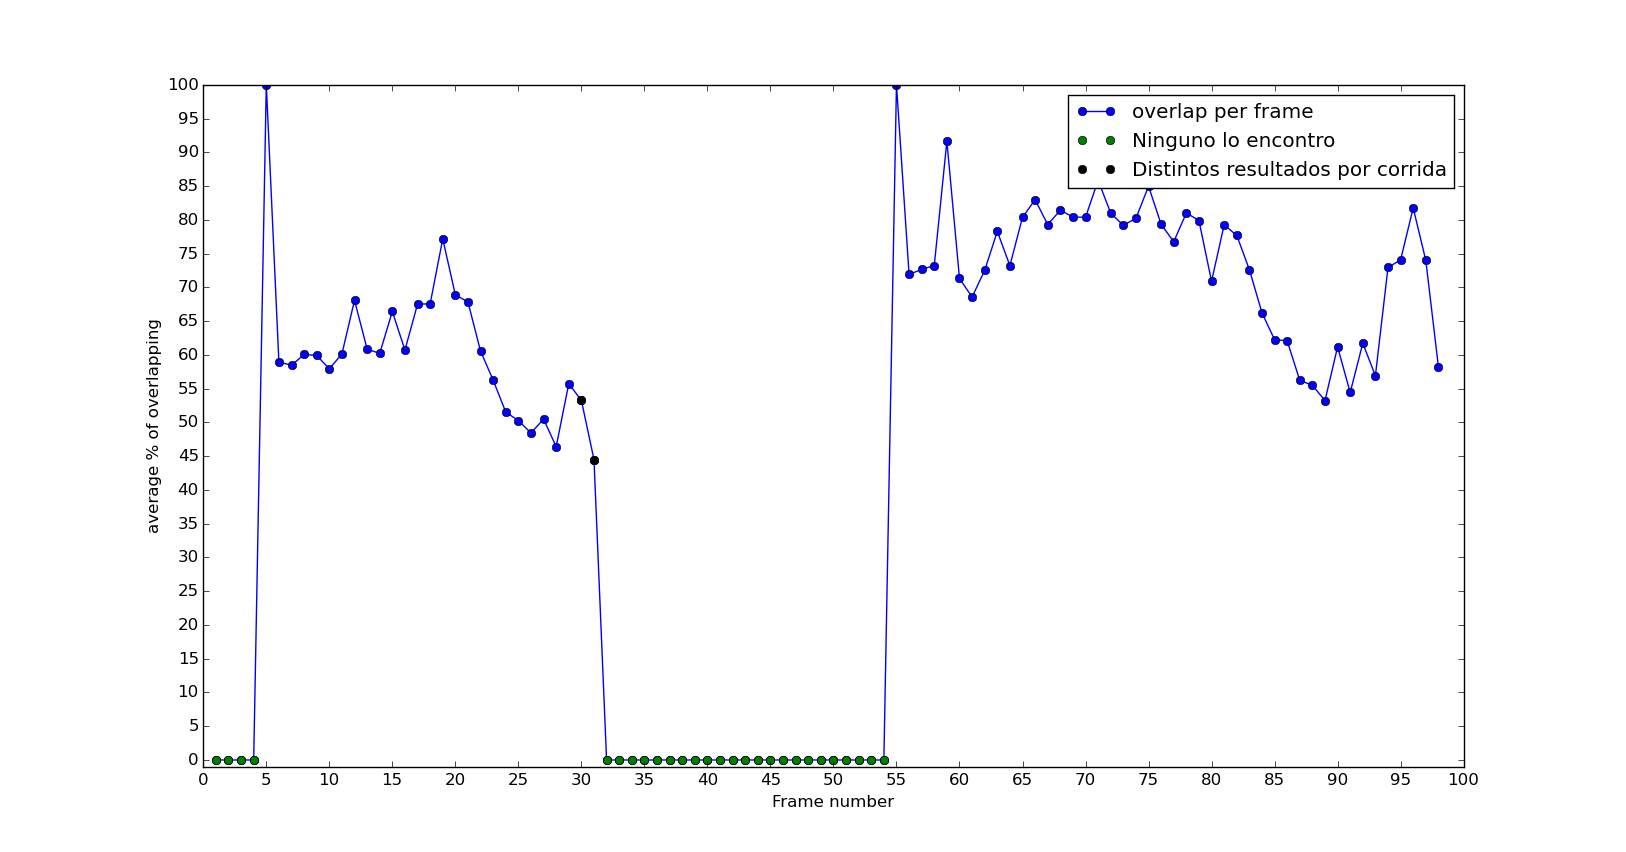
\includegraphics[width=\textwidth]{img/frame_a_frame/depth-taza.png}
		\caption{Seguimiento frame a frame para la taza}
		\label{frame_frame_d_taza}
	\end{subfigure}
	\begin{subfigure}[b]{0.9\textwidth}
		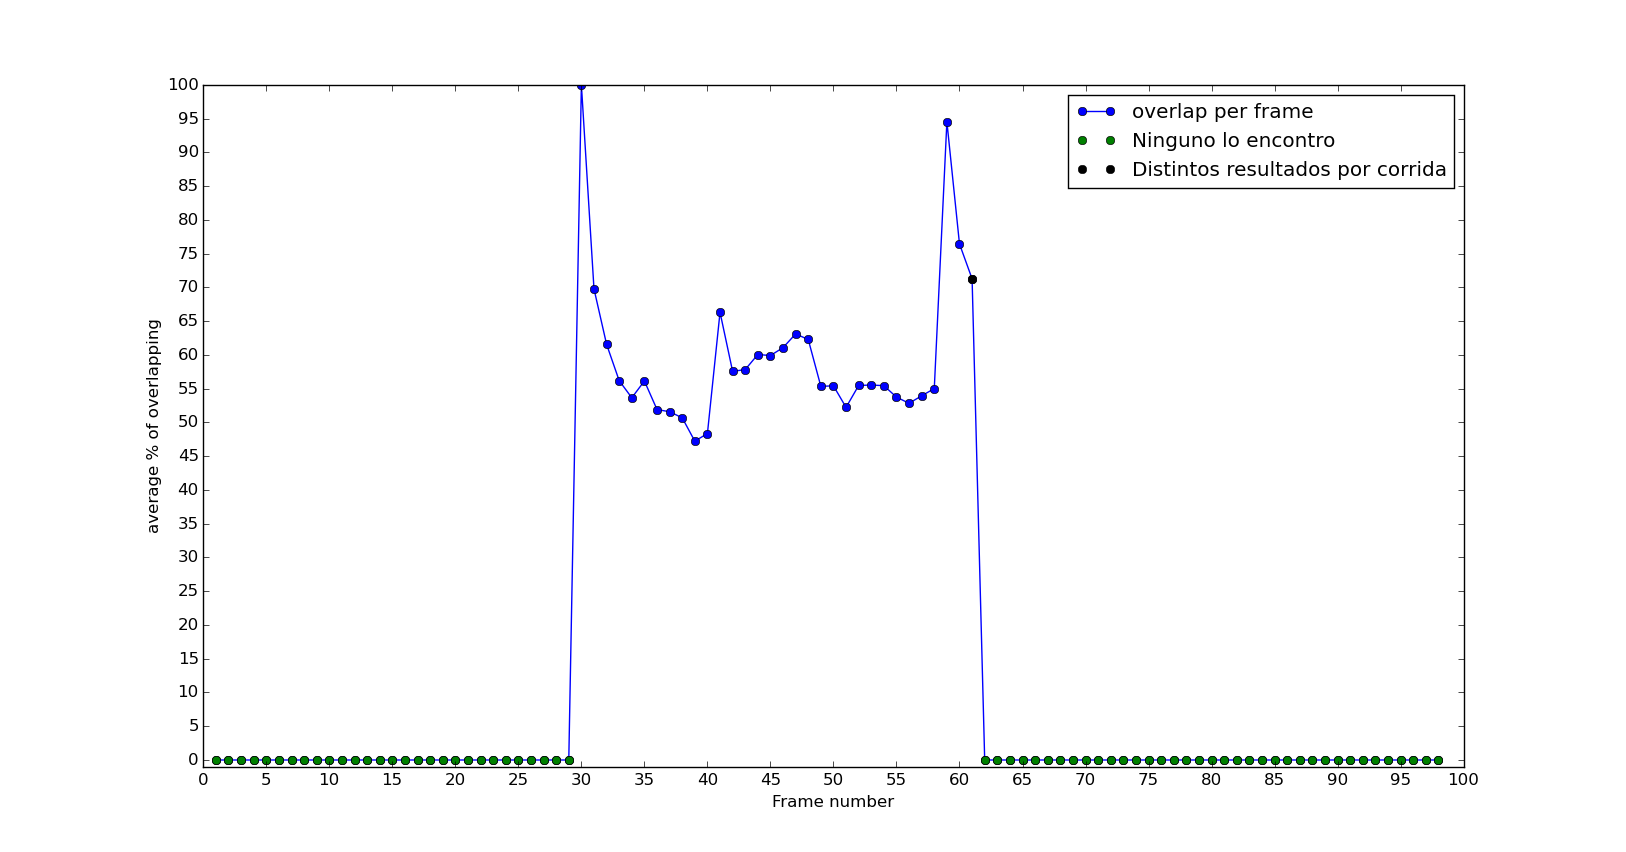
\includegraphics[width=\textwidth]{img/frame_a_frame/depth-gorra.png}
		\caption{Seguimiento frame a frame para la gorra}
		\label{frame_frame_d_gorra}
	\end{subfigure}
	\begin{subfigure}[b]{0.9\textwidth}
		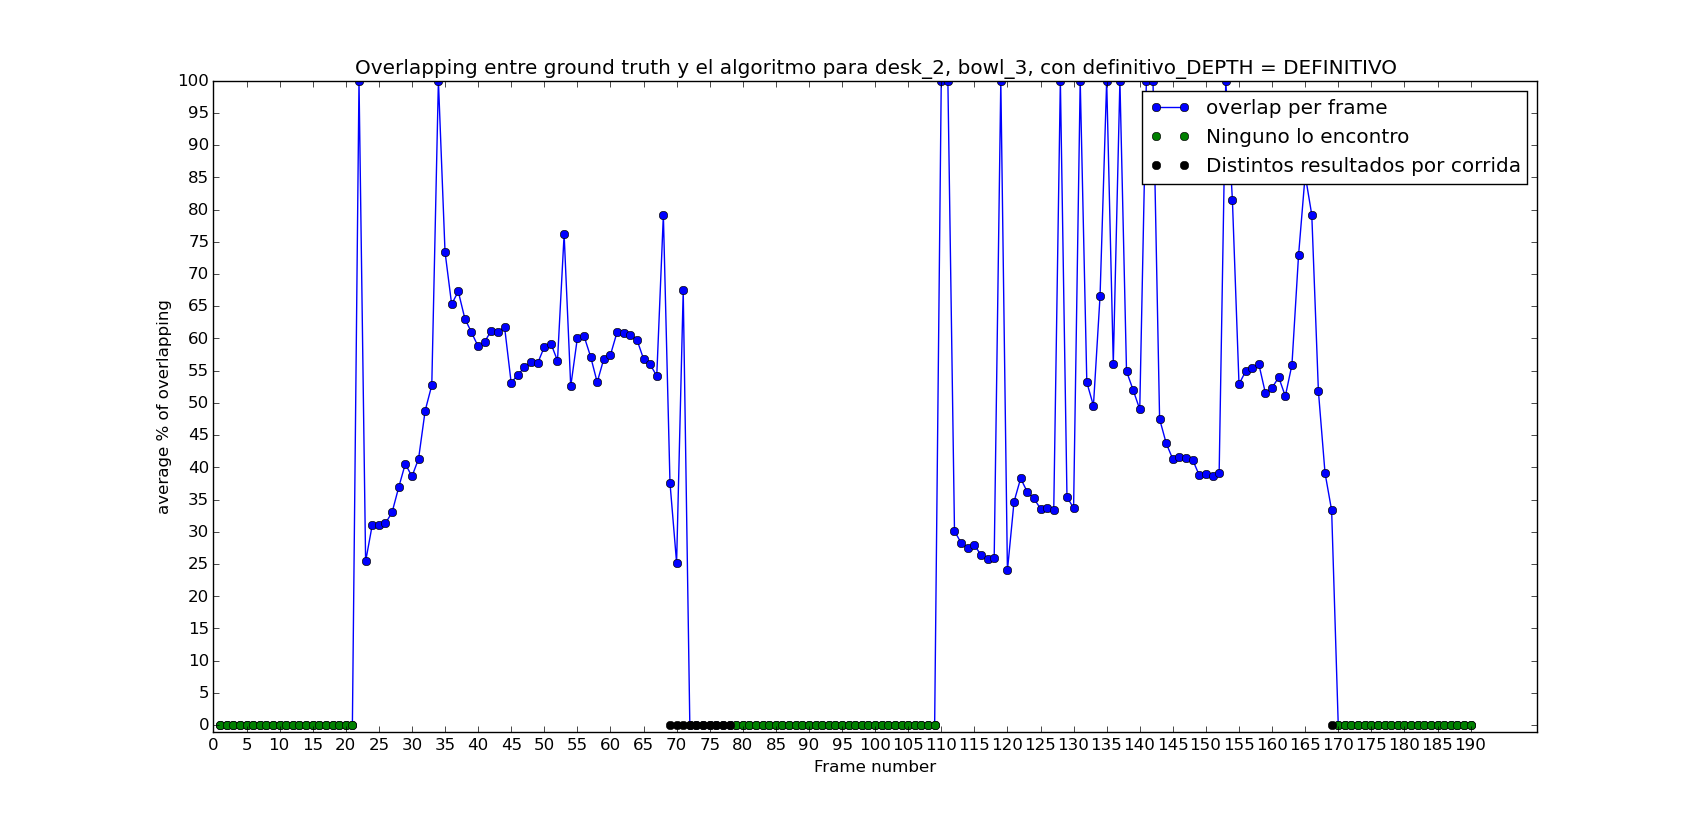
\includegraphics[width=\textwidth]{img/frame_a_frame/depth-bowl.png}
		\caption{Seguimiento frame a frame para el bowl}
		\label{frame_frame_d_bowl}
	\end{subfigure}
	\caption{Seguimiento frame a frame del tracking en profundidad con detección ideal.}
	\label{frame_frame_d}
\end{figure}


\section{Evaluación del tracking en RGB-D}
Una vez analizados el tracking en RGB y en profundidad por separado decidimos unir ambos métodos y corroborar como se comporta el tracking combinado. Como se explicó en la sección \ref{metodo_rgbd} la combinación se hizo de dos maneras distintas por lo que en el análisis también distinguiremos cada una de las combinaciones por separado.

\customsubsubsection{Tracking RGB-D con preferencia en profundidad}
La primera combinación que analizaremos es la que le da prioridad al tracking en profundidad y que utiliza el tracking RGB solo para intentar mejorar el resultado obtenido con profundidad. En la Tabla \ref{tabla_rgbd_d} vemos como se modificaron los promedios de solapamiento con respecto a la Tabla \ref{tabla_d}.

\begin{table}[h]
	\centering
    \begin{tabular}{|c|c|c|c|c|c|}
    \hline
    & \multirow{2}{2.4cm}{\% promedio de overlap} & \multirow{2}{2cm}{\% veces seguido} & \multirow{2}{1.6cm}{Falsos Positivos} & \multirow{2}{1.6cm}{\% Falsos Negativos}\\
	Objeto & & & &\\
    \hline
    Taza   & 65.07      & 90.05     & 0        &   1.7 \\
    \hline
    Gorra  & 42.83      & 90.82     & 0        &  1.02 \\
    \hline
    Bowl   & 42.88      & 68.54     & 1.75     &  11.4 \\
    \hline
    \end{tabular}
\caption{Resultados del tracking RGB-D utilizando la detección ideal, priorizando el tracking en profundidad.}
\label{tabla_rgbd_d}
\end{table}

En el único caso que mejoró el promedio de solapamiento es el de la taza en donde mejoró poco menos de un 1\%. En los casos de la gorra y el bowl empeoraron cerca de un 8\% y un 4\% respectivamente. Sin embargo en los tres casos se mejoró el porcentaje de seguimiento, haciendo más eficiente a este método combinado. Además, en esta tabla también puede verse que en el caso del bowl disminuyó la cantidad de falsos positivos y falsos negativos en comparación con el tracking exclusivamente para profundidad. En la Figura \ref{frame_frame_rgbd_d} se muestra como fue el seguimiento frame a frame para este método.

\begin{figure}
	\centering
	\begin{subfigure}[b]{0.9\textwidth}
		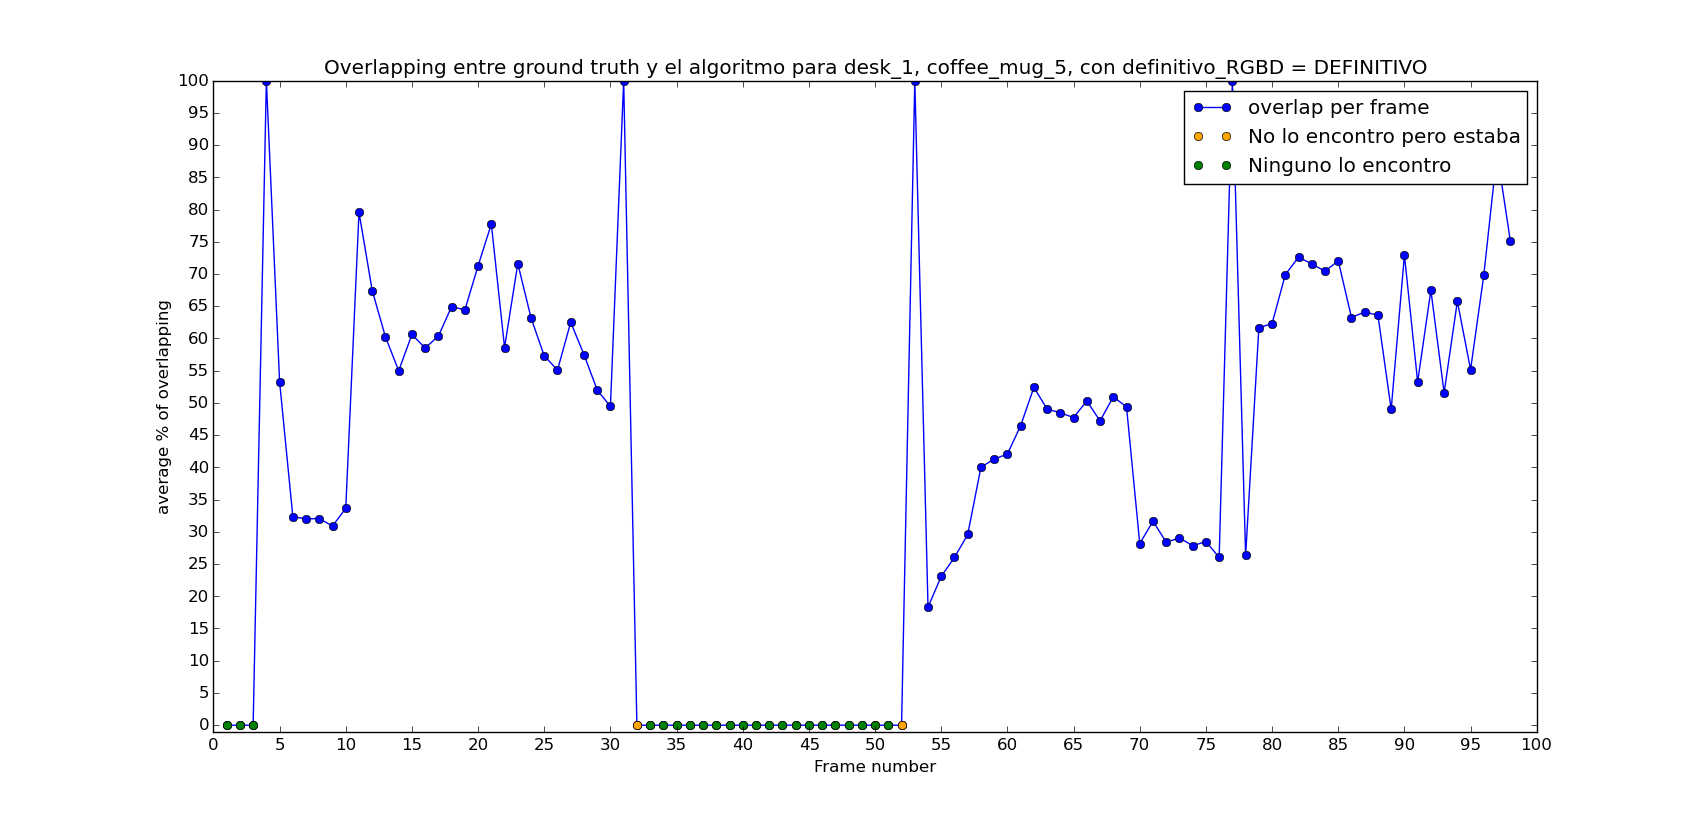
\includegraphics[width=\textwidth]{img/frame_a_frame/rgbd-d-taza.png}
		\caption{Seguimiento frame a frame para la taza}
		\label{frame_frame_rgbd_d_taza}
	\end{subfigure}
	\quad
	\begin{subfigure}[b]{0.9\textwidth}
		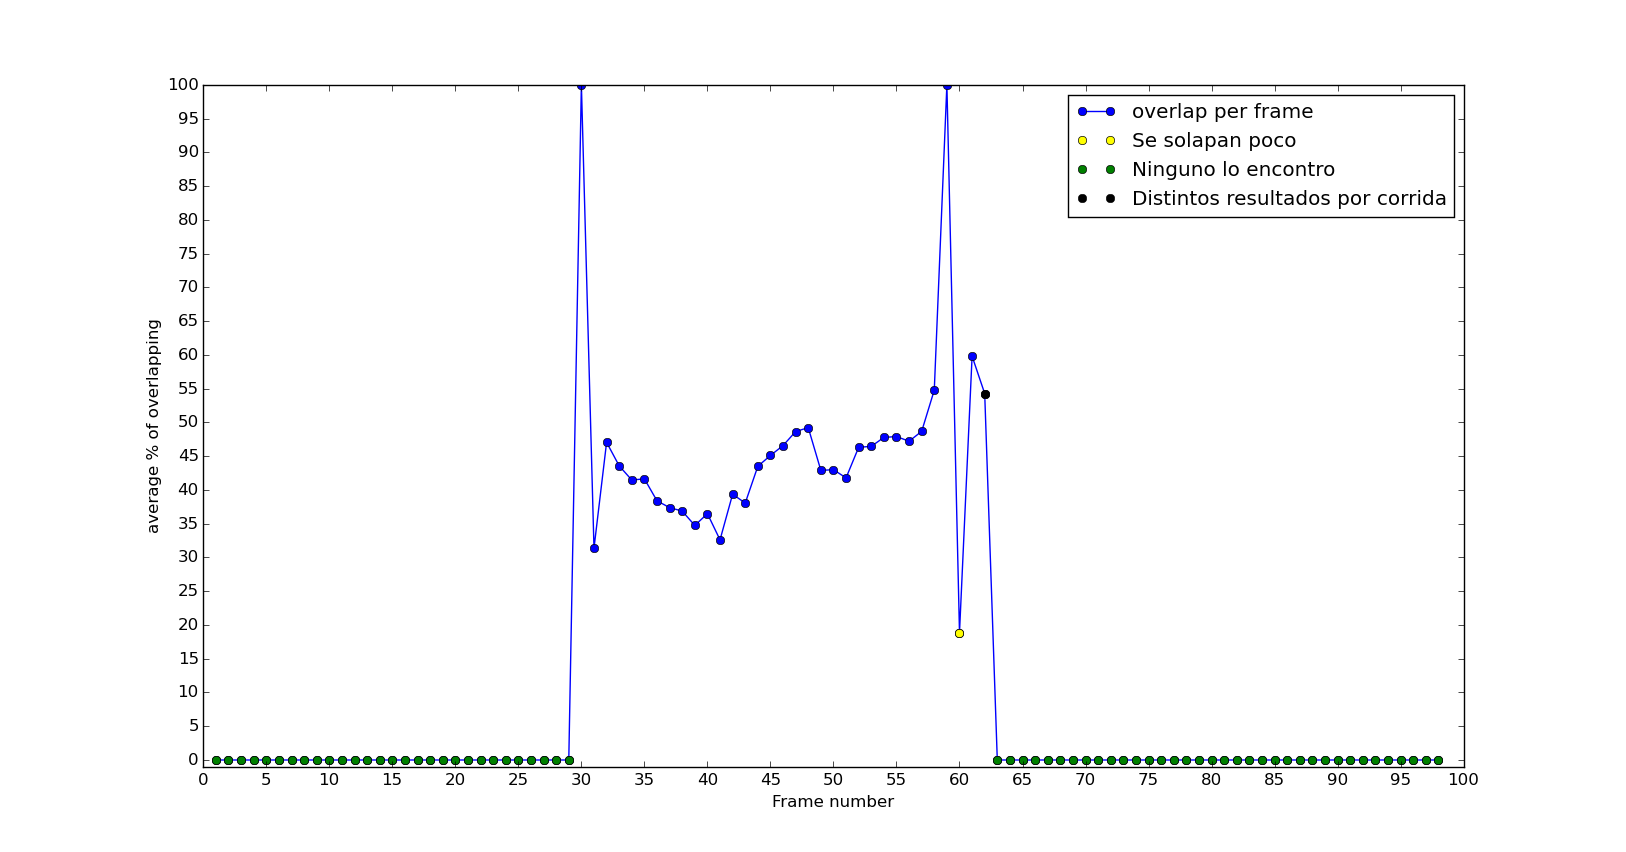
\includegraphics[width=\textwidth]{img/frame_a_frame/rgbd-d-gorra.png}
		\caption{Seguimiento frame a frame para la gorra}
		\label{frame_frame_rgbd_d_gorra}
	\end{subfigure}
	\quad
	\begin{subfigure}[b]{0.9\textwidth}
		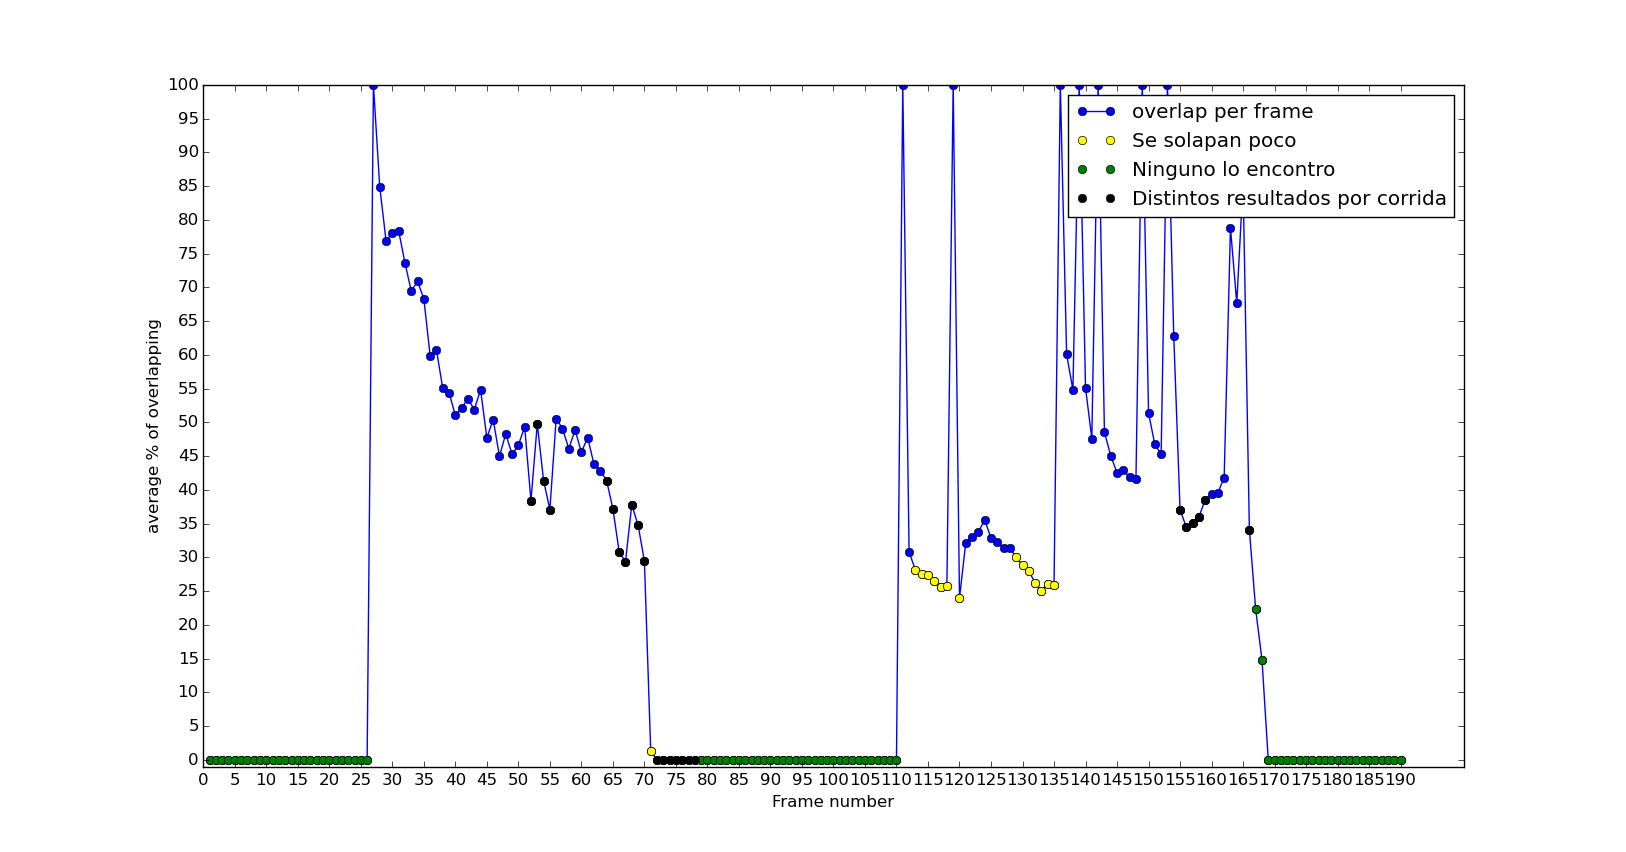
\includegraphics[width=\textwidth]{img/frame_a_frame/rgbd-d-bowl.png}
		\caption{Seguimiento frame a frame para el bowl}
		\label{frame_frame_rgbd_d_bowl}
	\end{subfigure}
	\caption{Seguimiento frame a frame para el tracking RGB-D con preferencia en profundidad usando la detección ideal.}
	\label{frame_frame_rgbd_d}
\end{figure}

Una hipótesis sobre la marcada diferencia del porcentaje de solapamiento entre el tracking RGB-D y usando solo profundidad es la manera en que se hace la comparación de histogramas entre el área de búsqueda del frame actual y uno de los templates del objeto. \comentarioM{Ver frames 42, 57 de la primer corrida y frames 57, 58, 60 de la tercera} Para esta comparación, como se explicó en la sección \ref{tracking_rgb}, se toma uno de los templates del objeto obtenido en la etapa de entrenamiento y se calcula su histograma. Como la gorra es casi totalmente roja, el histograma RGB va a estar claramente marcado por la presencia del color rojo. En cambio, en el recuadro reportado por el tracking en profundidad no solo aparece parte o la totalidad del objeto sino que además se incluye parte del fondo del recuadro en donde se encuentra el objeto. Al igual que en el seguimiento RGB, el algoritmo se ve perjudicado por no poder aislar al objeto del fondo de la imagen.

En la Figura \ref{mejora_rgb_en_tracking_rgbd} se pueden ver los distintos recuadros analizados por la mejora RGB, el recuadro del frame anterior y el template del objeto utilizado en la comparación. Se marca además cuál es el recuadro del frame actual elegido como el mejor según la comparación RGB.

\begin{figure}
	%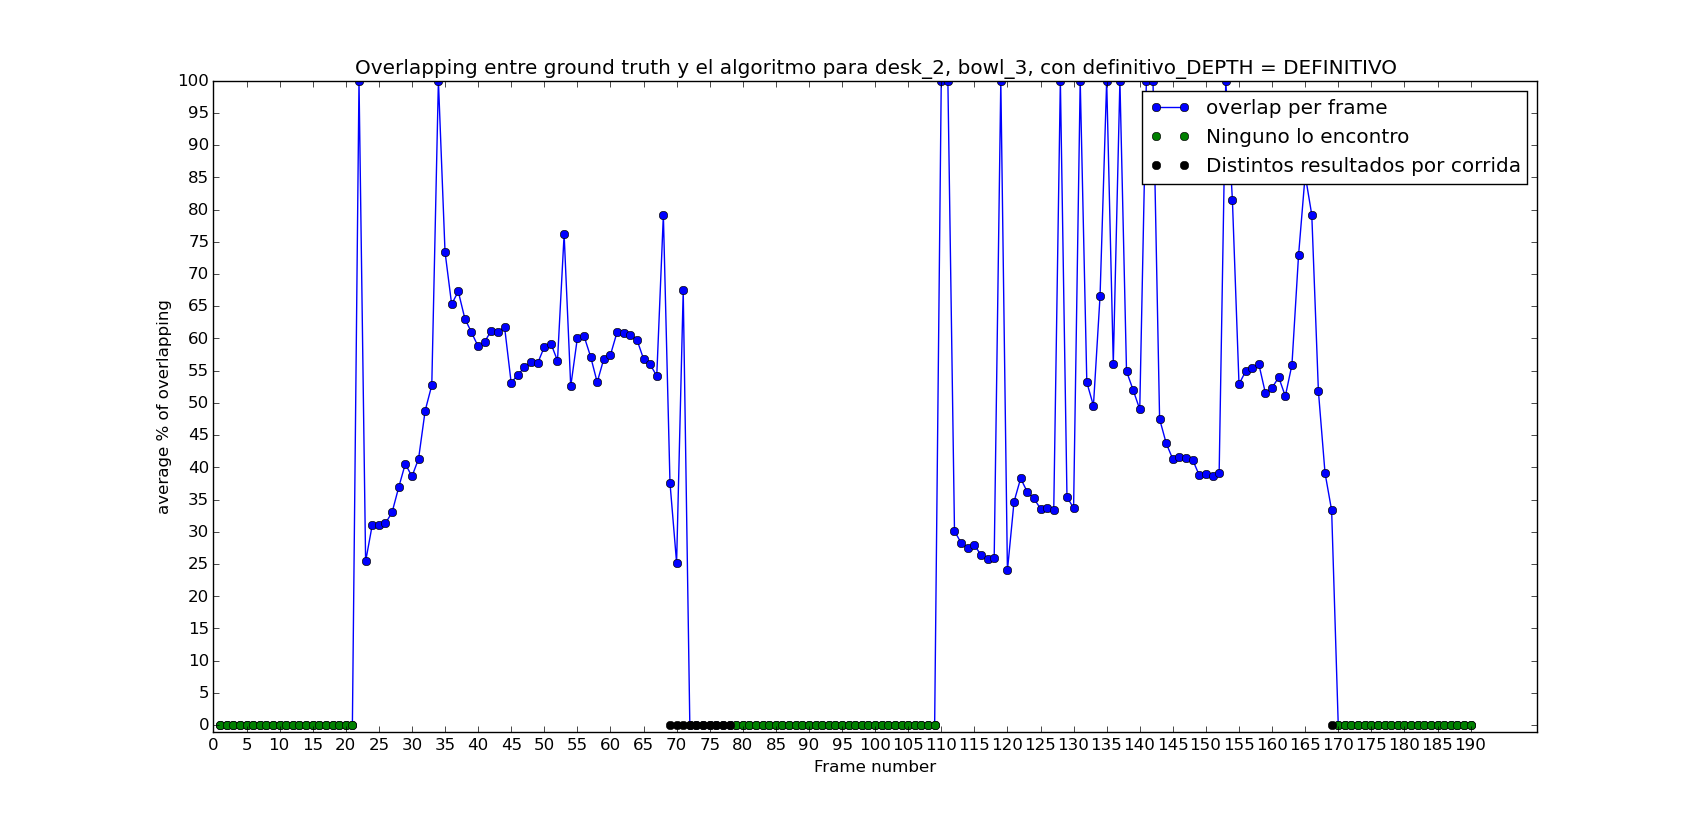
\includegraphics[width=\textwidth]{img/frame_a_frame/depth-bowl.png}
	\caption{Mejora obtenida según RGB para el tracking RGB-D}
	\label{mejora_rgb_en_tracking_rgbd}
\end{figure}

Una posible mejora para este algoritmo podría ser que durante el entrenamiento se obtenga una máscara por cada template del objeto que lo aisle del fondo de la imagen. Luego, utilizar estas máscaras para calcular los histogramas de los recuadros del frame anterior y del actual. De esta manera, si la pose del objeto en estos recuadros coincide con alguna de las poses de los templates la comparación va a ser más robusta y permitiría evitar este tipo de inconvenientes en la mejora RGB.

\customsubsubsection{Tracking RGB-D con preferencia en RGB}
La segunda combinación para el tracking RGB-D es la que le da prioridad al tracking RGB e intenta mejorar el resultado utilizando el tracking en profundidad. Esta combinación se explica en detalle en la sección \ref{tracking_rgbd}.

\begin{table}[h]
	\centering
    \begin{tabular}{|c|c|c|c|c|c|}
    \hline
    & \multirow{2}{2.4cm}{\% promedio de overlap} & \multirow{2}{2cm}{\% veces seguido} & \multirow{2}{1.6cm}{Falsos Positivos} & \multirow{2}{1.6cm}{\% Falsos Negativos}\\
	Objeto & & & &\\
    \hline
    Taza   & 50.48      & 83.10     & 0      & 8.16  \\
    \hline
    Gorra  & 63.91      & 96.94     & 0      & 0     \\
    \hline
    Bowl   & 13.39      &  6.87     & 0      & 13.33 \\
    \hline
    \end{tabular}
\caption{Resultados del tracking RGB-D utilizando la detección ideal, priorizando el tracking RGB.}
\label{tabla_rgbd_rgb}
\end{table}


Como se puede observar en la Tabla \ref{tabla_rgbd_rgb} y si se comparan los resultados con los de la Tabla \ref{tab:tabla_rgb}, podemos observar una notoria mejora en la escena de la gorra. Para este objeto se mejoró en casi 13 puntos el porcentaje el promedio de solapamiento de áreas casi sin variar el porcentaje de veces que se utilizó el tracking en toda la escena. Sin embargo el análisis para los otros dos objetos no varió mucho con respecto al seguimiento RGB.

Este resultado parece reafirmar la hipótesis hecha en la primera combinación RGB-D. En ese caso lo que vimos fue una baja importante en el porcentaje de solapamiento en comparación con el tracking en profundidad para el caso de la gorra. Aquí parece suceder al revés: el algoritmo de seguimiento en RGB reporta un área pequeña dentro de la superficie de la gorra que se ve en la imagen RGB y a la hora de correr la mejora en profundidad, esta trata de alinear la nube de puntos del frame anterior en la nube que proviene de tomar el resultado de RGB y proyectarlo en la escena en profundidad. Como esta alineación es exitosa, el área reportada por el tracking en profundidad proyectada en RGB es más grande que la reportada por el tracking RGB y por lo tanto se asemeja más a la indicada por el ground truth que contiene en el recuadro a la superficie de la gorra. Todo esto permite verificar una mejora en el seguimiento cuando se utilizan los datos en RGB-D en contraposición con el seguimiento exclusivamente en RGB.




\section{Evaluación de los métodos de tracking en objetos desconocidos}
Las pruebas analizadas hasta el momento fueron todas realizadas con los mismos objetos y son estos los que se utilizaron durante la selección de métodos y luego la de parámetros. En esta sección se analizarán pruebas corridas utilizando objetos nuevos y escenas nuevas, con los mismos métodos y parámetros de las secciones anteriores:
\begin{itemize}
	\item Detección ideal y seguimiento RGB
	\item Detección ideal y seguimiento en profundidad
	\item Detección ideal y seguimiento RGB-D, en sus dos combinaciones
\end{itemize}

Estas pruebas se realizaron con el objetivo de verificar el funcionamiento de los algoritmos en condiciones diferentes.

\begin{figure}
	\centering
	\begin{subfigure}[b]{0.3\textwidth}
		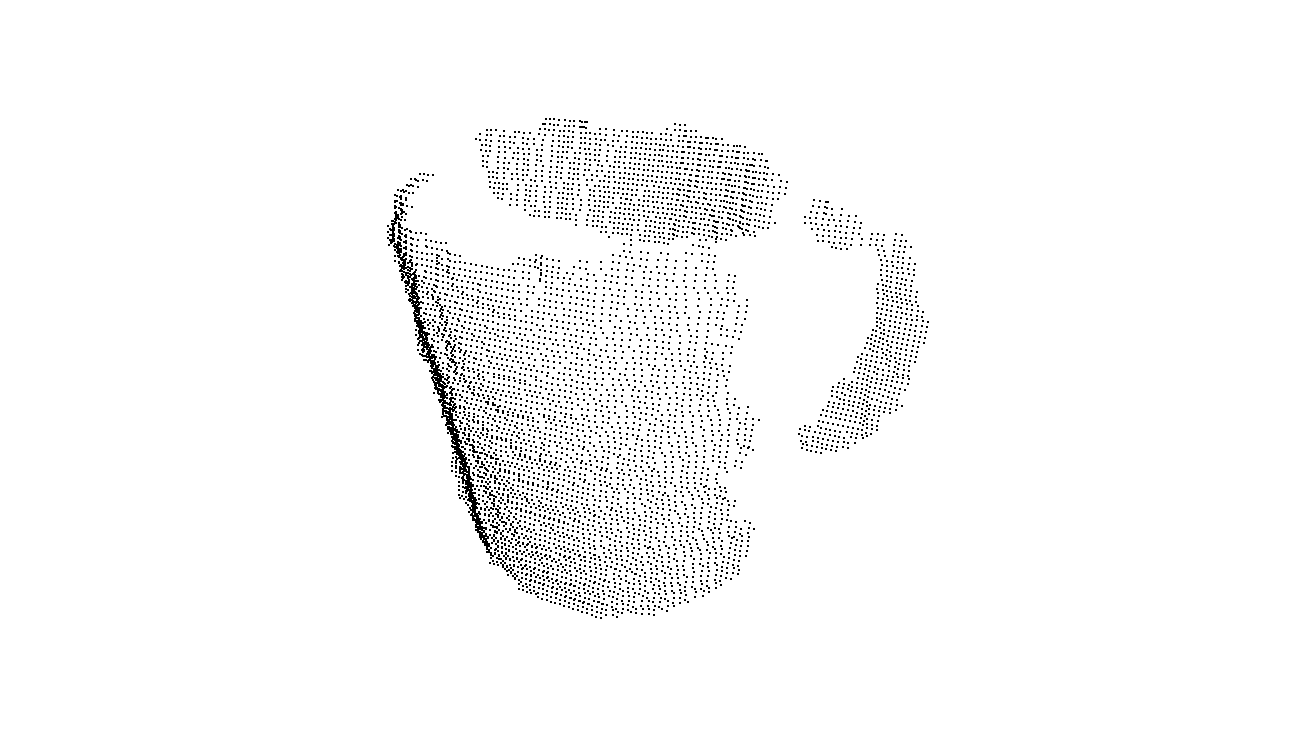
\includegraphics[width=\textwidth]{img/obj_nuevos/coffee_mug_pcd.png}
		\caption{Taza 2}
	\end{subfigure}
	\quad
	\begin{subfigure}[b]{0.3\textwidth}
		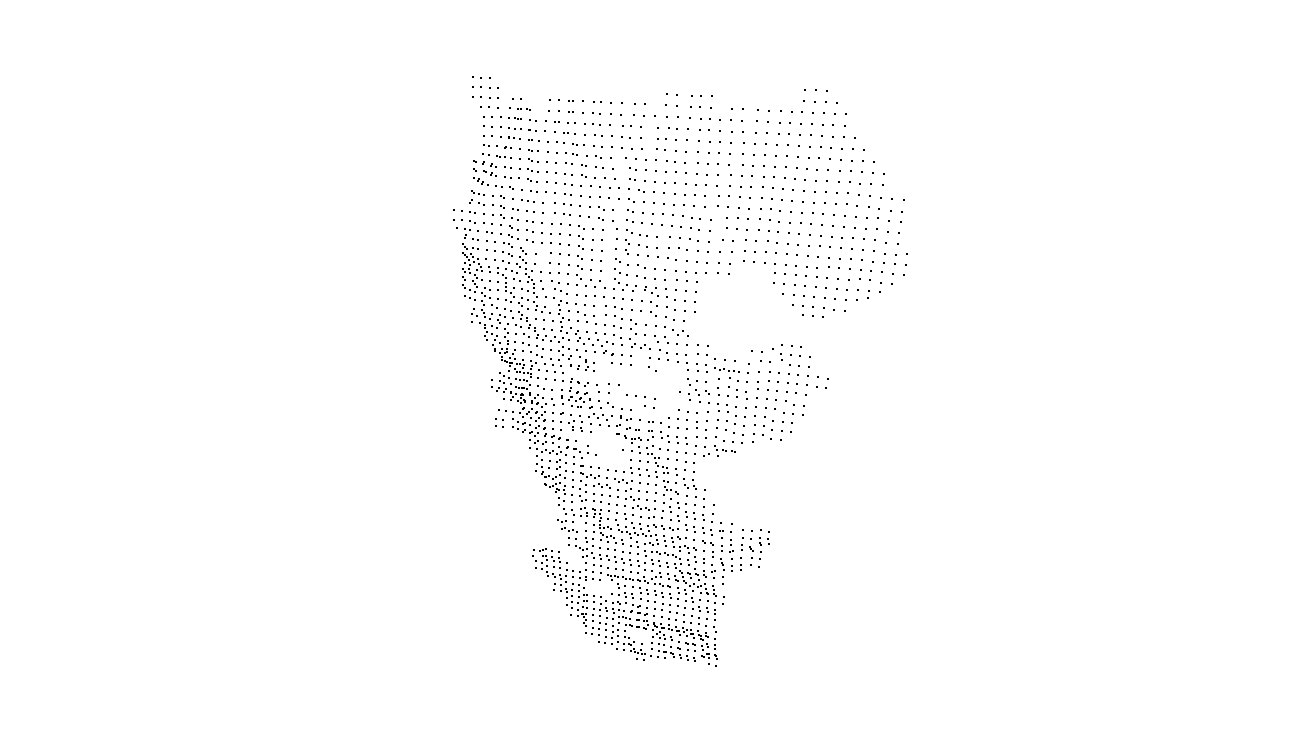
\includegraphics[width=\textwidth]{img/obj_nuevos/soda_can_pcd.png}
		\caption{Lata de gaseosa}
	\end{subfigure}
	\quad
	\begin{subfigure}[b]{0.3\textwidth}
		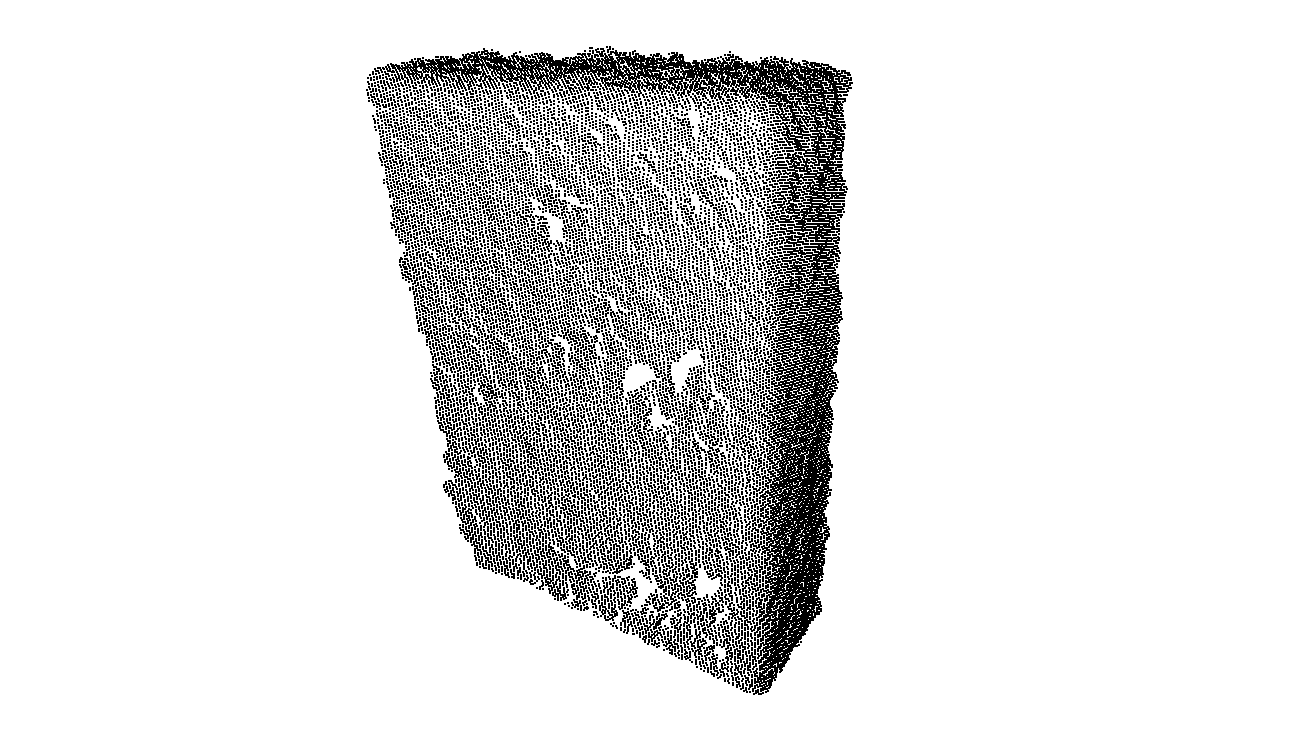
\includegraphics[width=\textwidth]{img/obj_nuevos/cereal_box_pcd.png}
		\caption{Caja de cereales}
	\end{subfigure}

	\caption{Objetos no utilizados durante las pruebas y selección de parámetros}
	\label{new_objects}
\end{figure}

Los objetos elegidos están entre los listados en la Figura \ref{fig:ejemplo_objetos_base}. En la Figura \ref{new_objects} se muestra para cada uno una nube de puntos de una única vista de cada objeto. Estos tienen distintas características y fueron elegidos bajo las siguientes hipótesis:
\begin{enumerate}
	\item Caja de cereales (ver Subfigura \ref{fig:caja}): al ser mayoritariamente plana debería perjudicar al tracking en profundidad y por su textura bien definida beneficiar al tracking RGB
	\item Lata de gaseosa (ver Subfigura \ref{fig:lata}): posee una textura bien definida pero el fondo de la imagen es oscuro al igual que la lata por lo que debería perjudicar al tracking RGB. Tiene una nube de puntos bastante plana. Al parecer no tiene una superficie que beneficie al sensor RGB-D. Esto debería perjudicar al seguimiendo en profundidad.
	\item Taza 2 (ver Subfigura \ref{fig:taza2}): es una taza diferente a la analizada antes. La forma debería beneficiar al tracking en profundidad y sus colores a RGB.
\end{enumerate}

Las escenas anotadas en donde se utilizaron estos objetos para correr los algoritmos y evaluar su comportamiento son distintas a las usadas con los objetos anteriores. En este caso se usaron dos: una es table\_1, en donde predomina una mesa grande rectangular sobre una esquina de una habitación donde un lado está sobre una pared y el otro debajo de una ventana (ver Subfigura \ref{fig:table_1}). En esta se encuentran entre otros objetos la lata y la taza 2. La otra también es sobre una mesa, llamada table\_small\_2, pero esta es una mesa circular y pequeña en el centro de una habitación pegada a una columna (ver Subfigura \ref{fig:table_small_2}). En esta escena es donde aparece la caja de cereales.


Teniendo en cuenta esta nueva selección de objetos y escenas y el motivo por el cual se eligió cada uno de ellos, analizaremos como se comportan los algoritmos en estos casos. En la Tabla \ref{tabla_rgb_nuevos} se pueden observar los resultados de estas pruebas.

\begin{table}[h]
	\centering
    \begin{tabular}{|c|c|c|c|c|c|}
    \hline
    & \multirow{2}{2.4cm}{\% promedio de overlap} & \multirow{2}{2cm}{\% veces seguido} & \multirow{2}{1.6cm}{Falsos Positivos} & \multirow{2}{1.6cm}{\% Falsos Negativos}\\
	Objeto & & & &\\
    \hline
    Taza 2  & 29.54      &  35.9     & 0        &  16 \\
    \hline
    Lata    &  0.01      &     0     & 12.8     &  52 \\
    \hline
    Caja    & 52.11      & 67.62     & 0        &   0 \\
    \hline
    \end{tabular}
\caption{Resultados del tracking RGB utilizando la detección ideal para objetos nuevos.}
\label{tabla_rgb_nuevos}
\end{table}

Como se esperaba, el algoritmo se comportó muy mal en el caso de la lata. Durante toda la escena el algoritmo reportó encontrar la lata en una zona que no se solapa con la reportada por el ground truth haciendo que el porcentaje de solapamiento sea muy bajo. En el caso de la nueva taza, el algoritmo funcionó de manera muy similar al caso de la taza que se utilizó durante el proceso de pruebas y selección de parámetros. En cuanto a la caja de cereales respecta, el algoritmo funcionó muy bien. A pesar del porcentaje relativamente bajo de veces que se siguió al objeto, las veces en las que hubo seguimiento el porcentaje de solapamiento fue bastante alto, como se puede ver en la Figura \ref{frame_frame_rgb_nuevo}. Un inconveniente que sufrió el algoritmo para esta escena es que la caja de cereales entre los frames 136 y 185 cambia la pose y en vez de estar de frente pasa a estar de costado (ver Figura \ref{fig:caja_de_costado}). Esto provoca que el histograma que describe a la caja en esos frames cambie mucho con respecto al del template que está tomado de frente y de esta manera el seguimiento reporta no encontrar al objeto. Si no se tienen en cuenta esos frames, el porcentaje de veces que se utiliza el algoritmo de seguimiento pasaría a ser de un 89\%.

\begin{figure}
	\centering
	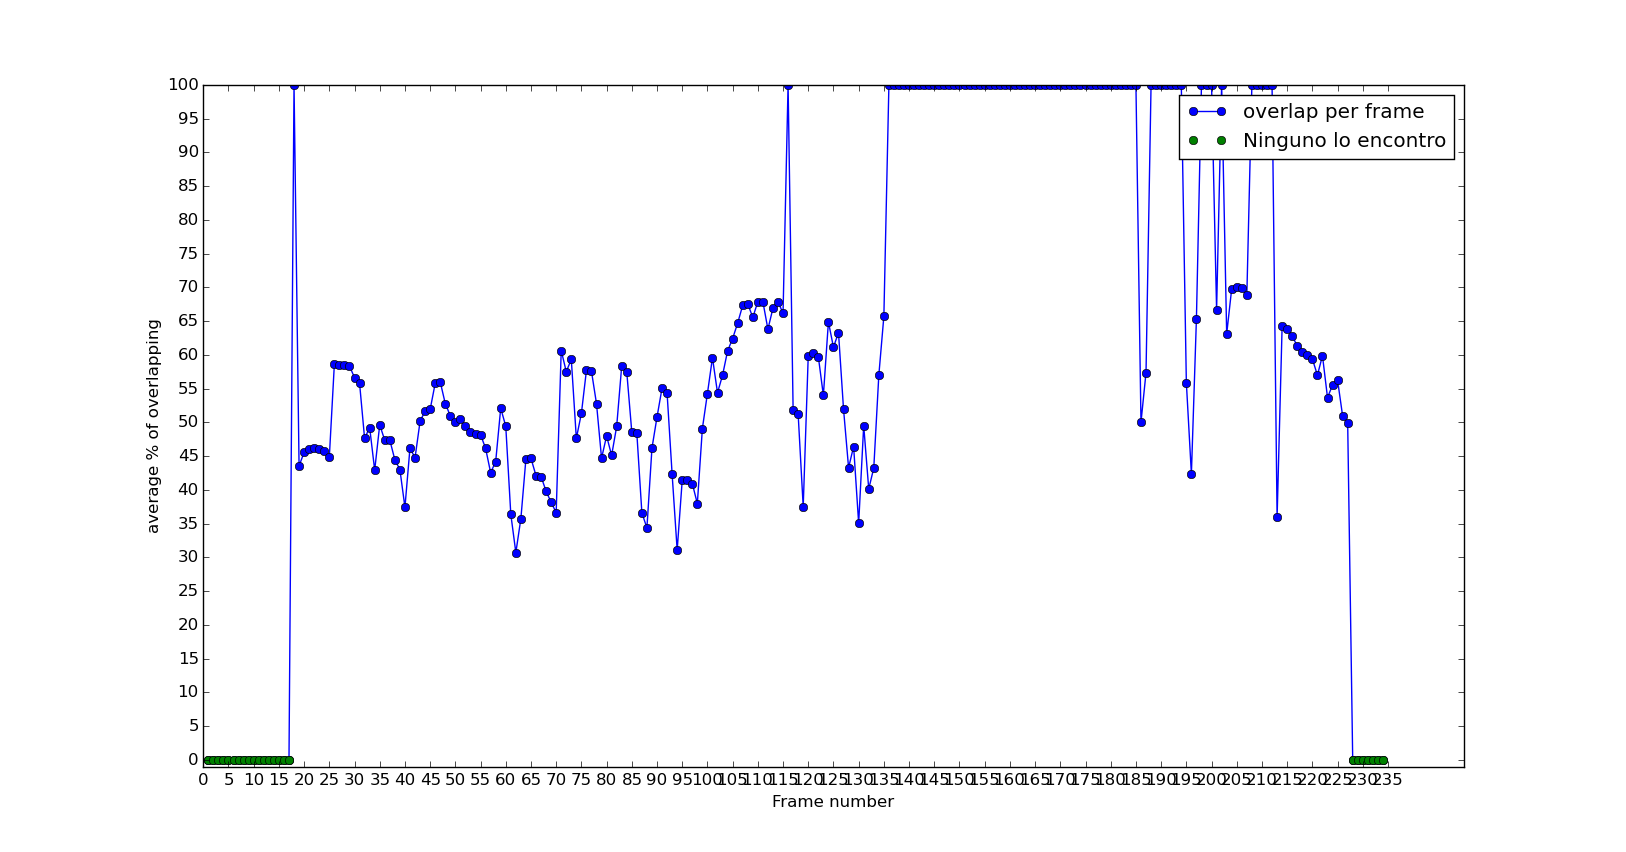
\includegraphics[width=\textwidth]{img/frame_a_frame/rgb-caja.png}
	\caption{Seguimiento frame a frame para la caja de cereales según el tracking en RGB}
	\label{frame_frame_rgb_nuevo}
\end{figure}



\begin{table}[h]
	\centering
    \begin{tabular}{|c|c|c|c|c|c|}
    \hline
    & \multirow{2}{2.4cm}{\% promedio de overlap} & \multirow{2}{2cm}{\% veces seguido} & \multirow{2}{1.6cm}{Falsos Positivos} & \multirow{2}{1.6cm}{\% Falsos Negativos}\\
	Objeto & & & &\\
    \hline
    Taza 2  & 55.79      & 80.51     & 0.27     &   1.2 \\
    \hline
    Lata    & 12.34      & 10.63     & 28.8     &    46 \\
    \hline
    Caja    & 44.94      & 30.62     & 0        & 11.97 \\
    \hline
    \end{tabular}
\caption{Resultados del tracking en profundidad utilizando la detección ideal para objetos nuevos.}
\label{tabla_d_nuevos}
\end{table}

En la Tabla \ref{tabla_d_nuevos} se ven los resultados del análisis del tracking en profundidad para estos nuevos objetos.
Para el ejemplo de la taza nueva el algoritmo se comporta de manera similar a la que lo hizo con la taza de las pruebas de selección de parámetros.

En el caso de la lata los resultados no fueron buenos. El problema principal es que el modelo de la lata es muy malo. Al tener partes que reflejan la luz infrarroja del sensor RGB-D, la información de profundidad de la lata no se captura de manera correcta obteniendo por cada vista de la lata una nube de puntos casi plana y con sectores en donde claramente faltan puntos que describan bien su superficie. Esto hace que la alineación durante el seguimiento sea mala y alinee el modelo con cualquier objeto plano de la escena, como por ejemplo la superficie de la mesa.

Finalmente, en el caso de la caja de cereales vemos que el algoritmo tiene un bajo porcentaje de veces que siguió al objeto. Si se observa la Figura \ref{frame_frame_d_nuevo}, debemos separar el análisis en tres partes. Por un lado, desde el inicio de la escena hasta el frame 136 el algoritmo funciona correctamente con un porcentaje de solapamiento promedio cercano al 45\% y una alta tasa de seguimiento. Luego, entre el frame 136 y el frame 185 sucede lo mismo que con el tracking RGB: el cambio de pose de la caja hace que el seguimiento falle y siempre se utilice la detección. Por último, entre el frame 185 y el fin de la escena el algoritmo vuelve a tener un buen porcentaje de solapamiento promedio y una tasa de seguimiento aceptable.

Tanto el caso de la lata como el de la caja de cereales muestran la importancia que tiene obtener un buen modelo del objeto durante el entrenamiento. En algunas ocasiones es dificil tomar un buen modelo a partir de una única vista del objeto, que es el caso de estos dos objetos.

\begin{figure}
	\centering
	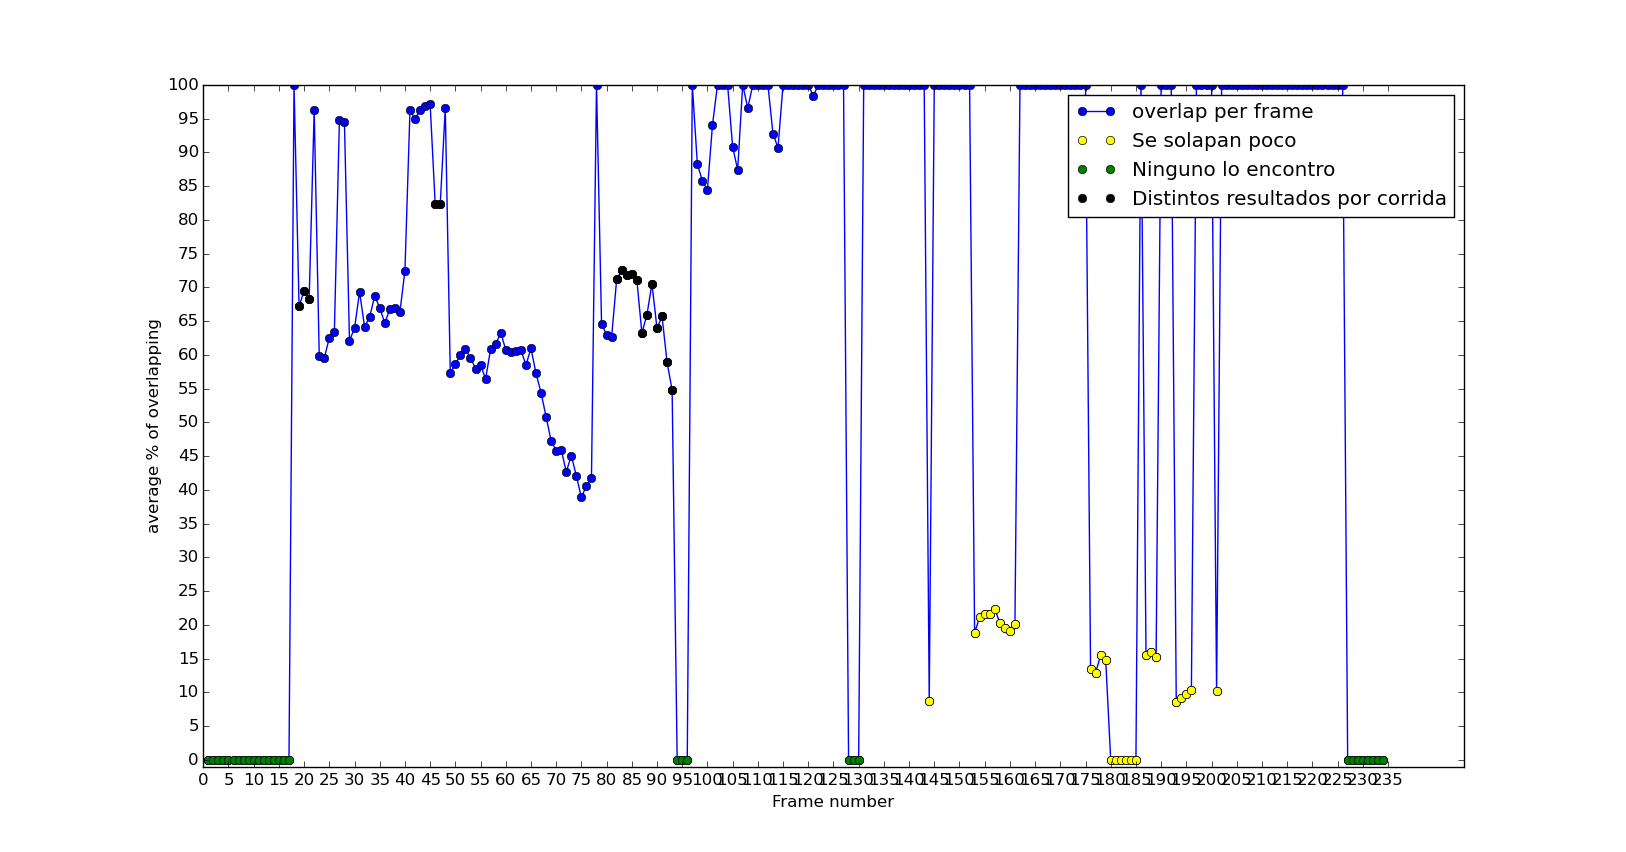
\includegraphics[width=\textwidth]{img/frame_a_frame/depth-caja.png}
	\caption{Seguimiento frame a frame para la caja de cereales según el tracking en profundidad}
	\label{frame_frame_d_nuevo}
\end{figure}


Finalmente analizamos los resultados de los algoritmos de tracking que combinan RGB con profundidad. Estos pueden verse en las tablas \ref{tabla_rgbd_d_nuevos} y \ref{tabla_rgbd_rgb_nuevos}. En ambos casos los resultados son casi identicos a cada uno de los algoritmos por separado. Sólo se observan muy leves mejoras en la escena de la taza. Esto era esperado y se debe a que la forma de la taza, al igual que la vista de donde se obtuvo el modelo de la nube de puntos, son favorables al método de seguimiento en profundidad. Además, esta instancia de taza, la taza 2, posee texturas que facilitan el seguimiento basado en histogramas para RGB. El objeto entonces posee buenas características para ambos sistemas, motivo por el cuál se capturan mejores resultados al combinar los dos seguimientos.

\begin{table}[h]
	\centering
    \begin{tabular}{|c|c|c|c|c|c|}
    \hline
    & \multirow{2}{2.4cm}{\% promedio de overlap} & \multirow{2}{2cm}{\% veces seguido} & \multirow{2}{1.6cm}{Falsos Positivos} & \multirow{2}{1.6cm}{\% Falsos Negativos}\\
	Objeto & & & &\\
    \hline
    Taza 2  & 35.98      & 48.33      & 0.8     & 10.93 \\
    \hline
    Lata    & 18.81      & 23.67      & 29.33   & 37.07 \\
    \hline
    Caja    & 35.03      & 23.29      & 0       & 16.67 \\
    \hline
    \end{tabular}
\caption{Resultados del tracking RGB-D con preferencia en profundidad para objetos nuevos.}
\label{tabla_rgbd_d_nuevos}
\end{table}

\begin{table}[h]
	\centering
    \begin{tabular}{|c|c|c|c|c|c|}
    \hline
    & \multirow{2}{2.4cm}{\% promedio de overlap} & \multirow{2}{2cm}{\% veces seguido} & \multirow{2}{1.6cm}{Falsos Positivos} & \multirow{2}{1.6cm}{\% Falsos Negativos}\\
	Objeto & & & &\\
    \hline
    Taza 2  & 33.62      & 39.32      & 0       & 14.93\\
    \hline
    Lata    &  0.01      &     0      & 12.8    &  52.0\\
    \hline
    Caja    & 52.11      & 67.62      & 0       &     0\\
    \hline
    \end{tabular}
\caption{Resultados del tracking RGB-D con preferencia en RGB y detección ideal para objetos nuevos.}
\label{tabla_rgbd_rgb_nuevos}
\end{table}


\section{Análisis general de los métodos}
% RGB vs profundidad: gana profundidad salvo en la gorra que gana rgb. decir porque es mejor profundidad analizando problemas con los colores y la iluminacion
%
% RGB-D RGB vs. RGB: La refinacion con profundidad permite mejorar en todos los casos a los resultados de RGB solo. esto se ve notoriamente en el caso de la taza en donde casi se duplican los porcentajes de seguimiento y de solapamiento a la vez que disminuye del 30\% al 8\% los falsos negativos.
%
%
% RGB-D D vs. D: Los resultados son muy similares con la excepción de una disminución en el solapamiento en el caso de la gorra en RGB-D. Mejoran un poco los falsos positivos.
%
%
% RGB-D RGB vs.RGB-D D: Los resultados para la taza y la gorra son similares, siendo un poco mejor los de RGB-D D. Sin embargo en el caso del bowl el RGB-D D gana notoriamente.

De todos los análisis realizados hasta este momento podemos decir que cada uno de los algoritmos tiene sus ventajas y desventajas. Si comparamos los métodos de seguimiento de profundidad y de RGB por separado, vemos una notoria diferencia en favor del seguimiento en profundidad. De manera similar, la combinación de los métodos de seguimiento teniendo como método principal a RGB se comporta mejor que el método RGB solo. Esto se ve notoriamente en el caso de la taza en donde casi se duplican los porcentajes de seguimiento y de solapamiento a la vez que disminuye del 30\% al 8\% los falsos negativos. Estas comparaciones muestran que en los casos analizados el seguimiento en profundidad es mucho más robusto y preciso que en RGB para los algoritmos implementados.

Realizando esta comparación entre el seguimiento en profundidad solo y el seguimiento combinado entre RGB y profundidad, con este último como principal, no se notan diferencias sustanciales en los resultados. Por un lado, para la gorra hay una disminución notoria en el porcentaje de solapamiento en el caso de los métodos combinados. Sin embargo, el seguimiento combinado tiene en general para todos los objetos un porcentaje de falsos positivos más bajo.

Finalmente, si comparamos los dos métodos de seguimiento combinados, el método que tiene como principal seguimiento al seguimiento en profundidad supera al que tiene a RGB como principal. Esto se nota por un lado con la escena de la taza, en donde el porcentaje de solapamiento es de un 65\% contra el 50\% del que tiene RGB como principal incluso superándolo en porcentaje de veces seguido. Algo más notorio es en el caso del bowl en donde supera ampliamente en porcentaje de seguimiento y de solapamiento. El análisis de falsos positivos y falsos negativos también es muy favorable para el seguimiento combinado priorizando el método de profundidad.

Todas estas comparaciones se mantienen cuando hacemos el análisis de los resultados para los objetos que no se utilizaron durante la selección de parámetros, salvo en el caso de la comparación entre seguimiento en profundidad solo y el seguimiento combinado con el de profundidad como principal. Este último parece verse afectado por las correcciones hechas con el seguimiento RGB ya que, salvo en la escena de la lata, es superado por el seguimiento en profundidad notoriamente.

Con estos resultados podemos decir que el método de seguimiento en profundidad es en general mejor que el seguimiento en RGB, considerando los métodos elegidos en cada caso y para los objetos que se utilizaron durante los experimentos. En cuanto a la combinación de métodos creemos que es mejor utilizar aquella que prioriza el seguimiento en profundidad y es mejorado con RGB. Sin embargo, resulta clave poder combinar los métodos de manera de minimizar las ocasiones en que el intento de corrección del resultado con el método secundario, en este caso RGB, empeoren el resultado final. Si no se tiene un método de seguimiento RGB confiable, entonces es preferible utilizar un seguimiento basado unicamente en profundidad.


\section{Evaluación del sistema RGB-D}\label{sec:evaluacion_rgbd}
Para finalizar con la evaluación de los métodos, presentamos en esta sección los resultados para todas las escenas antes vistas correspondientes al sistema RGB-D explicado en la sección \ref{metodo_rgbd}.

En la Tabla \ref{tabla_sistema_rgbd} se puede ver un análisis similar al realizado anteriormente para cuantificar el comportamiento de los algoritmos de tracking. La principal diferencia es que en esta tabla se incluyen los resultados de las detecciones para el promedio de solapamiento y para el porcentaje de veces seguido, ya que en esta ocasión las detecciones son automáticas y por lo tanto nos interesa conocer el comportamiento del sistema de seguimiento en su totalidad. Además, se incluye el \textit{accuracy} como medida de cuantificación. El \textit{accuracy} es la proporción de resultados correctos sobre el total de los casos examinados. Su fórmula es la siguiente:
\begin{equation}
accuracy = \frac{\#TP + \#TN}{\#TP + \#TN + \#FP + \#FN}
\end{equation}

\begin{table}[h]
	\centering
    \begin{tabular}{|c|c|c|c|c|c|}
    \hline
    & \multirow{2}{2.4cm}{\% promedio de overlap} & \multirow{2}{2cm}{\% veces seguido} & \multirow{2}{1.6cm}{Falsos Positivos} & \multirow{2}{1.6cm}{Falsos Negativos} &\\
	Objeto & & & & & Accuracy\\
	\hline
    Taza    & 50.44      & 76.67     &    0           & 16.67    & 83.33 \\
    \hline
    Gorra   & 50.05      & 68.09     &    0           &  10.2    & 89.8 \\
    \hline
    Bowl    & 28.18      & 45.67     &    0           &  28.6    & 71.4 \\
    \hline
    Taza 2  & 45.54      & 77.78     &    0           &  6.93    & 93.07 \\
    \hline
    Lata    & 12.72      & 25.85     &   20           & 40.53    & 39.47 \\
    \hline
    Caja    &  6.17      &    10     &    0           & 73.08    & 26.92 \\
    \hline
    \end{tabular}
\caption{Resultados del sistema de seguimiento RGB-D}
\label{tabla_sistema_rgbd}
\end{table}


Como podemos ver, en las corridas de las dos tazas y la gorra el accuracy es alto, entre 83\% y 93\%. Esto significa que en el 83\% o 93\% de los frames el algoritmo reportó correctamente la presencia y ubicación del objeto. Además, en estos tres ejemplos el promedio de porcentaje de solapamiento está por encima del 45\% y el porcentaje de seguimiento por encima del 71\%.

Si comparamos los resultados del sistema con los resultados de cada método de seguimiento por separado vemos como nuestro sistema responde muy bien y en muchos casos superando a los otros métodos. Esto es un indicador de que la combinación de información RGB y de profundidad mejora la calidad de las detecciones y del seguimiento.

El seguimiento en RGB con detección ideal supera al sistema en el caso de la gorra, siendo 5 puntos mejor en el porcentaje promedio de solapamiento y cerca de 30 puntos más de porcentaje de seguimiento (ver tablas \ref{tab:tabla_rgb} y \ref{tabla_sistema_rgbd}). Esto se debe a la combinación de un modelo de nube de puntos de la gorra malo y el método de detección que resulta poco robusto. También es mejor en el caso de la caja de cereales, superando en 50 puntos tanto al porcentaje de solapamiento como al de veces que se siguió al objeto. En parte esto sucede por motivos similares al de la gorra, sumando que sobre la mitad de la escena y casi hasta el final, la caja queda de perfil a la cámara haciendo que el modelo 3D de la misma no sirva para alinearlo con la escena, y por lo tanto empeorando el rendimiento. Sin embargo, en el resto de las escenas, específicamente para ambas tazas, el bowl y la lata, el sistema supera ampliamente no solo al porcentaje de solapamiento promedio, sino también al porcentaje de veces que se sigue al objeto y el porcentaje de falsos positivos.

En el caso del seguimiento en profundidad, se nota cómo un buen método de detección, en este caso el método ideal, beneficia al algoritmo de seguimiento. Si comparamos los resultados de las Tablas \ref{tabla_d} y \ref{tabla_d_nuevos} del tracking en profundidad con los de la Tabla \ref{tabla_sistema_rgbd} del sistema RGB-D vemos que en la mayoría de los casos el seguimiento en profundidad con detección ideal supera ampliamente al sistema RGB-D en porcentaje de seguimiento y por bastante también en porcentaje promedio de solapamiento. Sólo en el ejemplo de la lata el sistema se comporta mejor. Sin embargo, el sistema demuestra ser mucho más robusto que el tracking en profundidad ya que mejora en todos los casos el porcentaje de falsos positivos.

A continuación presentamos los gráficos de seguimiento frame a frame para el sistema RGB-D de las escenas de la taza, la gorra y el bowl, en la Figura \ref{frame_frame_d}.

\begin{figure}
	\centering
	\begin{subfigure}[b]{0.9\textwidth}
		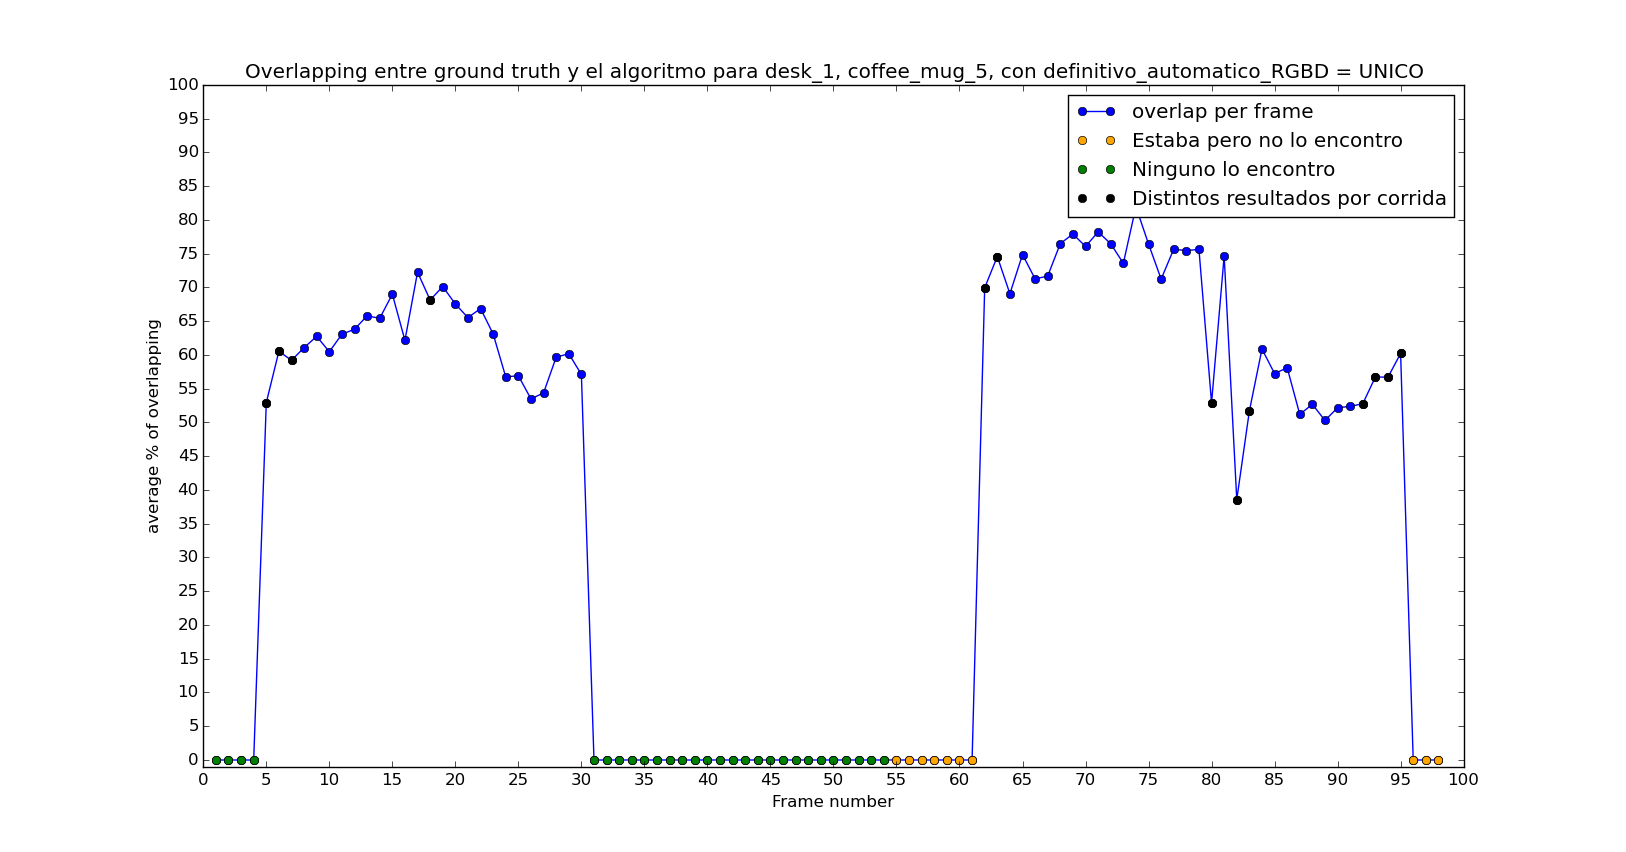
\includegraphics[width=\textwidth]{img/frame_a_frame/sistema-rgbd-taza.png}
		\caption{Seguimiento frame a frame para la taza}
		\label{frame_frame_sistema-rgb-d_taza}
	\end{subfigure}
	\quad
	\begin{subfigure}[b]{0.9\textwidth}
		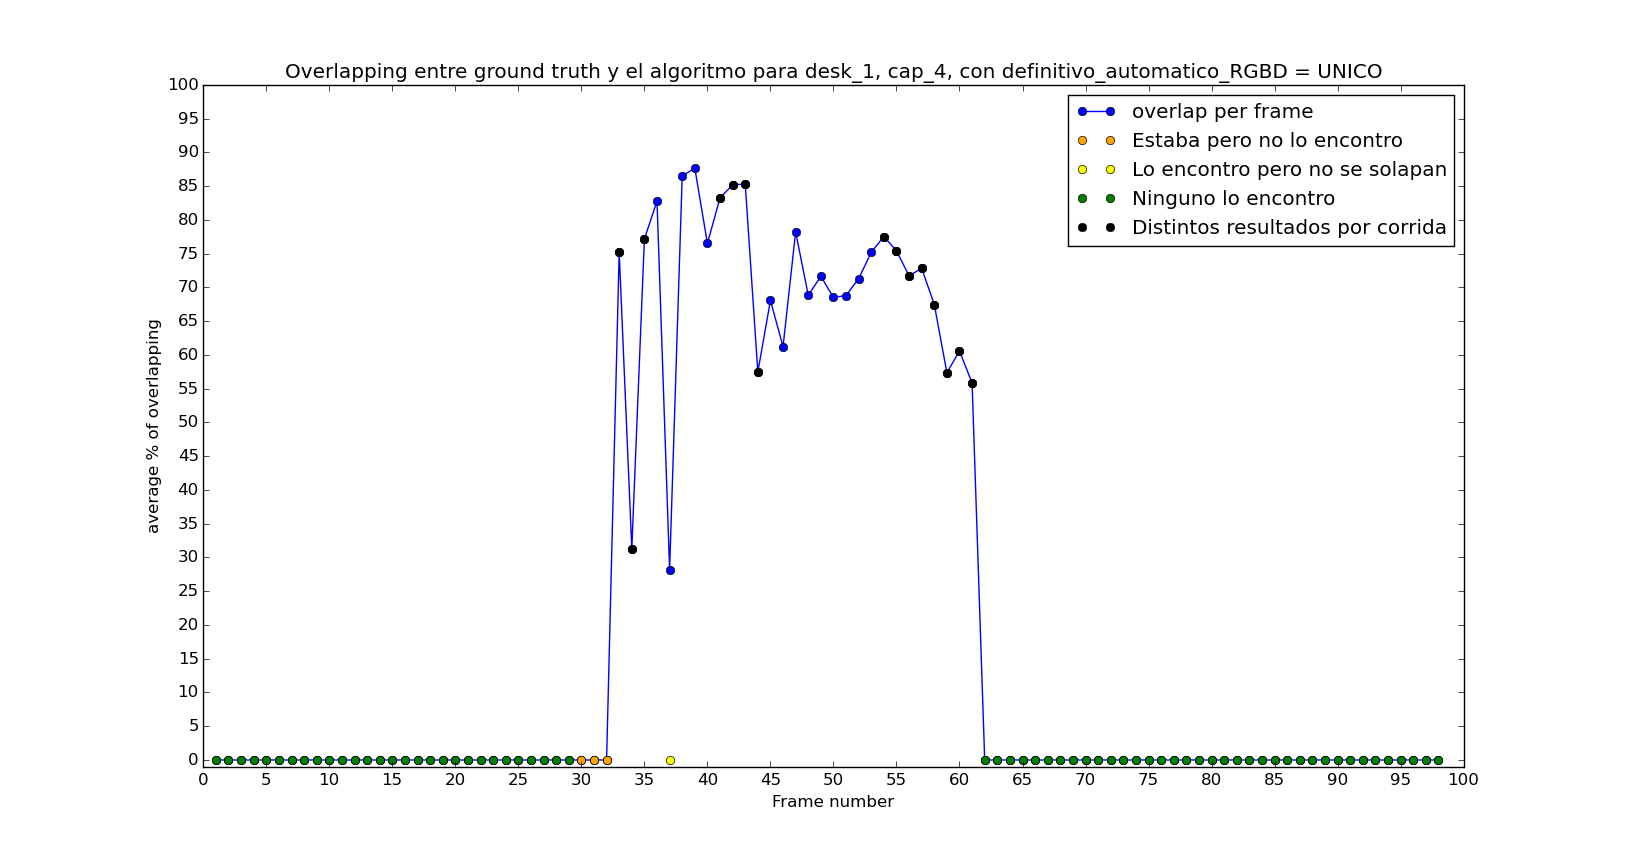
\includegraphics[width=\textwidth]{img/frame_a_frame/sistema-rgbd-gorra.png}
		\caption{Seguimiento frame a frame para la gorra}
		\label{frame_frame_sistema-rgb-d_gorra}
	\end{subfigure}
	\quad
	\begin{subfigure}[b]{0.9\textwidth}
		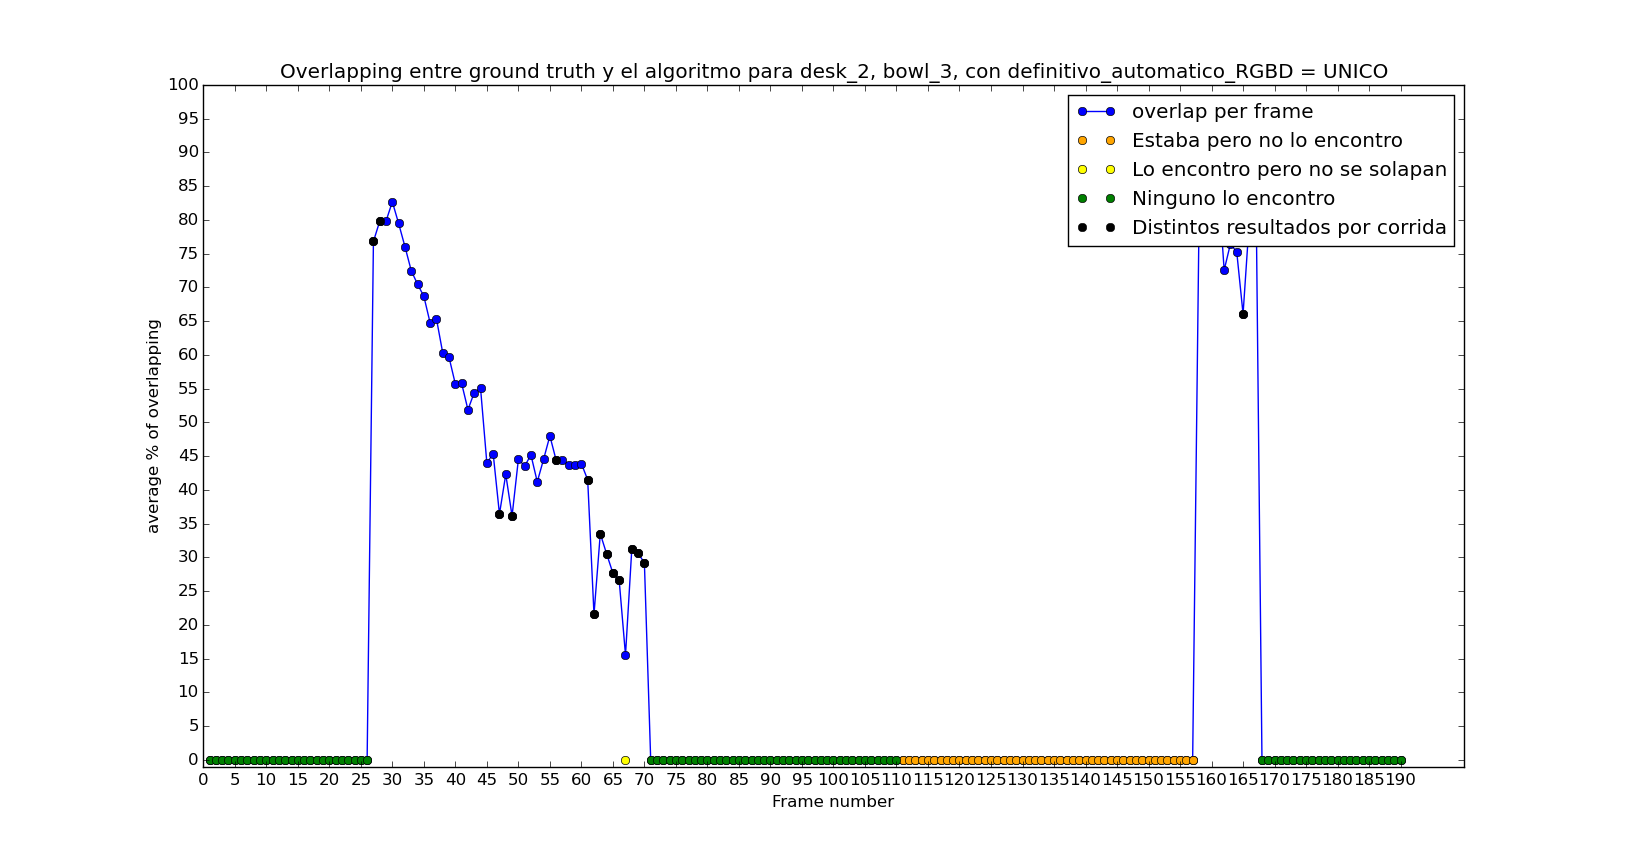
\includegraphics[width=\textwidth]{img/frame_a_frame/sistema-rgbd-bowl.png}
		\caption{Seguimiento frame a frame para el bowl}
		\label{frame_frame_sistema-rgb-d_bowl}
	\end{subfigure}
	\caption{Seguimiento frame a frame del sistema RGB-D}
	\label{frame_frame_d}
\end{figure}

Correspondiendose estos gráficos con los resultados presentados en la Tabla \ref{tabla_sistema_rgbd}, vemos como el sistema se comporta bien para las corridas de la taza y la gorra en las Subfiguras \ref{frame_frame_sistema-rgb-d_taza} y \ref{frame_frame_sistema-rgb-d_gorra}. En ambas subfiguras se observan pocos puntos de color negro lo que significa que el algoritmo es robusto.

En la Subfigura \ref{frame_frame_sistema-rgb-d_bowl} se distinguen tres etapas bien diferenciadas. Desde el inicio de la escena hasta el frame 110 el algoritmo se presenta muy robusto, comenzando con un buen porcentaje de solapamiento y decayendo a medida que se suceden los frames. Entre los frames 110 y 157 el algorimo de detección falla desmejorando notoriamente el comportamiento global del sistema. Finalmente, la tercera etapa comprendida entre el frame 157 y el final de la escena vuelve a ser buena como la primera etapa, logrando altos porcentajes de solapamiento y reportando bien la no presencia del bowl en la escena. Analizando la escena notamos que los frames en donde el algoritmo es robusto se corresponden con frames en donde el bowl está a una distancia cercana al sensor RGB-D y en donde la iluminación es buena. En cambio entre los frames 110 y 157 el sensor está algo lejos del bowl y al tomar la escena desde otro ángulo la iluminación es distinta y por lo tanto la cámara RGB devuelve imágenes con colores algo saturados, en ambos casos afectando a la detección.

A modo de saber que tan buena es la elección de umbral de solapamiento mínimo para considerar una detección como tal, es decir si se solapan en un porcentaje al menos igual al del umbral elegido, se hace un análisis del \textit{accuracy} del sistema variando los valores de dicho umbral. Se toman valores para el umbral que van desde 0\% hasta 100\% a una distancia de 0.1 entre cada umbral y se calcula el accuracy para cada objeto con cada uno de esos umbrales. En la Figura \ref{fig:accuracy_sistema} se observa este análisis en donde el umbral del 30\% utilizado durante este trabajo está marcado con una línea punteada.

\begin{figure}
	\centering
	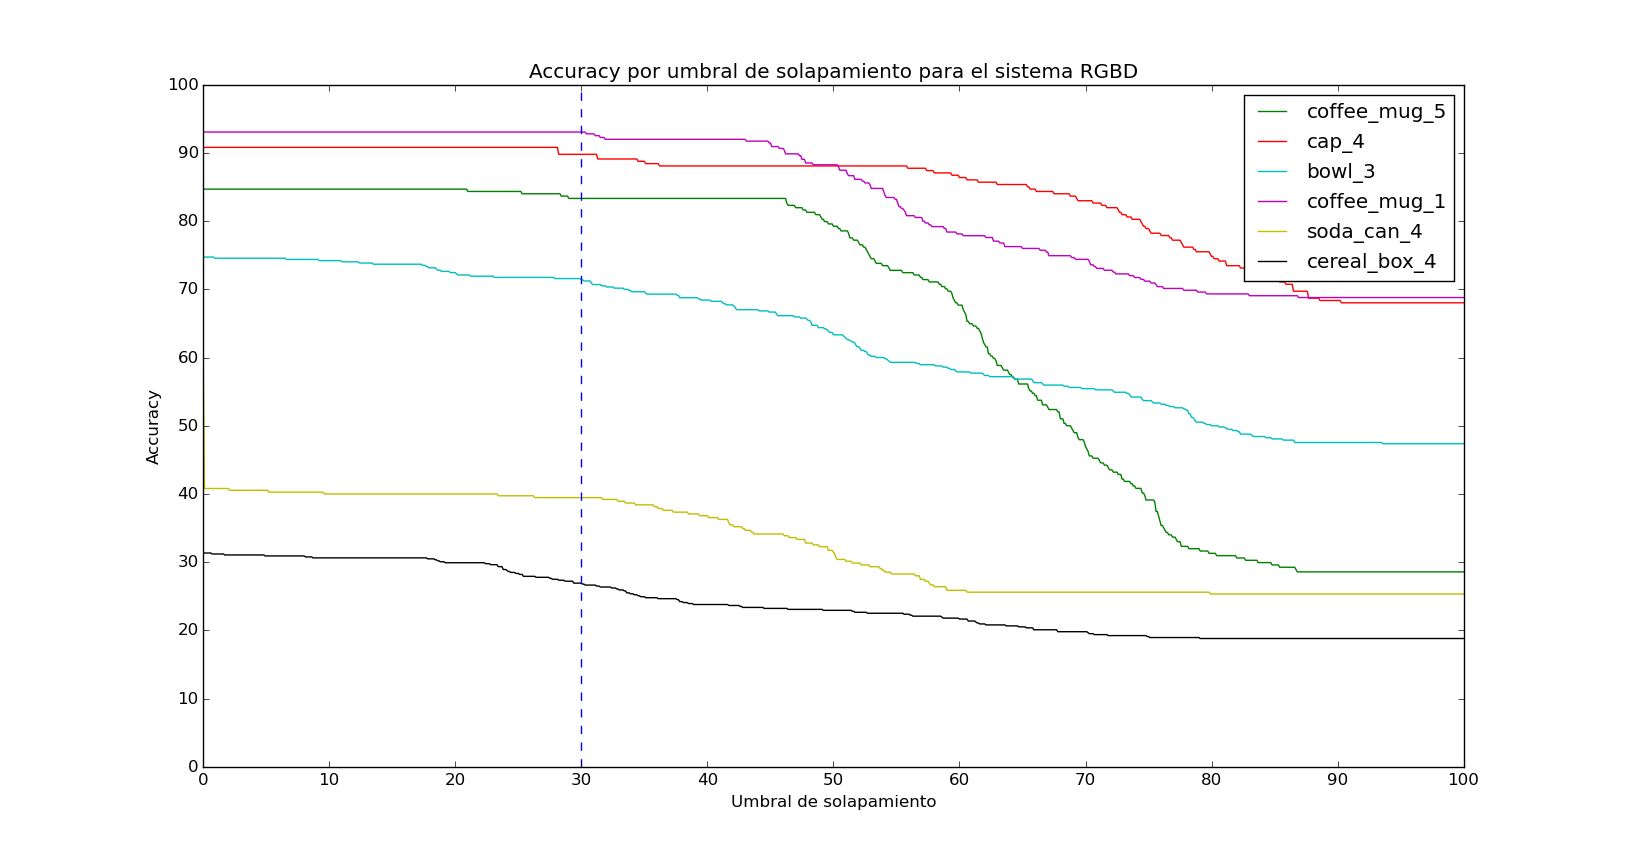
\includegraphics[width=\textwidth]{img/accuracy_sistemaRGBD.png}
	\caption{Análisis de accuracy según el umbral mínimo de solapamiento}
	\label{fig:accuracy_sistema}
\end{figure}

Para las escenas de las tazas y la gorra vemos que el accuracy se mantiene por encima del 85\% con un umbral de hasta 45\%. Para las escenas del bowl y la lata, un umbral del 30\% los mantiene por encima del 70\% y 40\% del accuracy respectivamente. El accuracy en la escena de la caja de cereales varía entre un 30\% y un 20\%. El máximo umbral que permite mantener un accuracy del 30\% es del 20\%. Con esto podemos determinar que el umbral elegido es bueno ya que sin permitir muy malas detecciones por poco solapamiento mantiene a la mayoría de los ejemplos con un accuracy por encima del 70\% y 80\%.


\chapter{Conclusiones}\label{chap:conclusiones}
Los resultados obtenidos durante la experimentación muestran en general un buen comportamiento del tracking en profundidad. Logramos obtener buenos porcentajes de solapamiento y de seguimiento con poca información sobre el objeto a seguir y además el método se adapta bien a las distintas formas de los objetos, aunque puede reportar malos resultados si el objeto a buscar es muy pequeño, está alejado del sensor RGB-D o si la nube de puntos del modelo del objeto es plana.

La combinación de métodos RGB y de profundidad para el seguimiento mejora la efectividad y robustez del seguimiento. Sin embargo, resulta de vital importancia combinar los métodos de manera de maximizar las ventajas de cada uno. Sería conveniente encontrar alguna manera de comparar el resultado obtenido con el método de profundidad y el obtenido al tratar de corregir este resultado con el método RGB. De esta manera se podría cuantificar la mejora otorgada por el seguimiento secundario y reportar el mejor de los dos resultados, tratando de afectar lo menos posible al resultado final.

Para un óptimo funcionamiento del sistema de seguimiento en general es de vital importancia contar con un método de detección robusto y eficaz. Los resultados obtenidos para nuestro sistema son buenos para la mayoría de los casos analizados pero si se los contrasta con los obtenidos con el método de detección ideal todos los valores analizados están muy por debajo de lo mejor que se puede obtener del método de seguimiento combinado propuesto. Una tarea a futuro es adaptar el trabajo realizado en \cite{hinterstoisser2010dominant} en nuestro sistema ya que combina una robusta y precisa detección con una performance de tiempo real.

Nuestro sistema de seguimiento tiene varias mejoras posibles para implementar. Una de ellas es hacer que el método de seguimiento sea robusto a oclusiones. Como se muestra en la Figura \ref{taza_ocluida} el método de seguimiento funciona correctamente pero solo reporta el área de la parte visible del objeto que se sigue, haciendo que el porcentaje de solapamiento con el área reportada por el ground truth sea menor al 50\%. Esto se puede resolver utilizando el filtro de Kalman \cite{welch1995introduction} adaptándolo al dominio 3D que utilizamos. El filtro de Kalman es un filtro muy popular y estudiado extensivamente en la literatura \cite{julier1997new,wan2000unscented} debido a su gran desempeño para realizar seguimiento en imágenes 2D.

Otra mejora a explorar está relacionada con la manera que comparamos histogramas RGB. Durante la etapa de búsqueda de valores de parámetros definimos un umbral máximo para la diferencia arrojada por la comparación de Bhattachayyra. Sin embargo este umbral sería mejor si se adaptara automáticamente según el tamaño, forma del objeto y color de fondo de la imagen. El resultado otorgado por el algoritmo tiene entre otras cosas las coordenadas en el dominio 2D de la imagen RGB de un cuadrante que contiene al objeto seguido. Dependiendo de la forma del objeto este cuadrante va a contener más o menos área que no sea parte del objeto sino de lo que existe alrededor del mismo. Si el fondo del objeto va cambiando durante la escena, el cálculo del histograma se ve afectado por este cambio y por lo tanto también lo va a hacer el resultado de la comparación con el histograma del template del objeto. Si a esto le agregamos que la forma del objeto es tal que el área que ocupa en el recuadro que lo contiene es pequeña, la diferencia de histogramas va a ser mayor aún ante cambios en el fondo de la imagen. Este problema provoca que se descarten buenos resultados al tener un umbral fijo.

Para obtener un sistema de seguimiento completamente automático hace falta implementar un algoritmo de segmentación de objetos en imágenes 3D para la etapa de entrenamiento, cuyo funcionamiento sea similar a lo hecho en el trabajo de Lepetit et al. \cite{park2011texture}. De esta manera se puede obtener una buena vista del objeto en 3D que sirva como modelo para el seguimiento en profundidad, a la vez que se toma la información en RGB para el seguimiento en 2D.

Como trabajo a futuro queda implementar todas estas técnicas de manera eficiente para lograr un seguimiento en tiempo real. Durante el desarrollo de este trabajo se tomaron recaudos en generar un código fuente que permitiera cambios rápidos para probar distintos métodos, ya sea de seguimiento, de detección, de entrenamiento, distintas variantes al esquema de seguimiento propuesto y combinaciones de los métodos en cada una de las etapas, pero en ningún momento se priorizó la performance por la claridad en el código. Tener una implementación que funcione en tiempo real sería de vital importancia si se quisiera usar este método en alguna aplicación real.



%%%% BIBLIOGRAFIA
\backmatter
\bibliographystyle{alpha}
\bibliography{tesis}

\end{document}



